%%%%%%%%%%%%%%%%%%%%%%%%%%%%%%%%%%%%%%%%%%%%%%%%%%%%%%%%%
% Niniejszy plik przedstawia przykładowy skład 
% pracy dyplomowej na Wydziale Matematyki PWr. 
% 
% Autorzy: 
% Damian Fafuła
% Michał Kijaczko
% Jakub Michalczak
% Maciej Miśta
% Dagmara Nowak
% Tomasz Skalski
% Wojciech Słomian
%
%% Data utworzenia: 8.05.2018
% Numer wersji: 1
%
% Poniższą formatkę można rozpowszechniać i edytować 
% pod warunkiem zachowania numeru wersji, 
% informacji o autorach i dodaniu informacji 
% o wprowadzonych zmianach.
%
%%%%%%%%%%%%%%%%%%%%%%%%%%%%%%%%%%%%%%%%%%%%%%%%%%%%%%%%%
% Domyślną opcją jest: praca magisterska, język polski.
% W przypadku pracy pisanej w języku angielskim dodajemy 
% opcję [english].
% Dla pracy licencjackiej dodajemy opcję [licencjacka].
% Dla pracy inżynierskiej dodajemy opcję [inzynierska].
% Dopuszczalne są podwójne opcje, np. [licencjacka, english].
% Opcje dodajemy w kwadratowym nawiasie przy \documentclass.
%
%
%%%%%%%%%%%%%%%%%%%%%%%%%%%%%%%%%%%%%%%%%%%%%%%%%%%%%%%%%
\documentclass[magisterska, english]{pwr_wmat_praca_dyplomowa}
%%%%%%%%%%%%%%%%%%%%%%%%%%%%%%%%%%%%%%%%%%%%%%%%%%%%%%%%%
%              DANE DO PRACY
%
% W przypadku pracy dyplomowej w języku angielskim nie jest konieczne 
% wypełnianie pól: \tytul{}, \kierunek{}, \specjalnosc{}, 
%                  \streszczenie{}, \slowakluczowe{}.
%%%%%%%%%%%%%%%%%%%%%%%%%%%%%%%%%%%%%%%%%%%%%%%%%%%%%%%%%
%
% Imię i nazwisko autora
\autor{Piotr Florek}
%
% Tytuł pracy dyplomowej 
\tytul{Tytuł pracy dyplomowej} 
\tytulang{Comparative analysis of gradient boosting algorithms used for classification problems}
%
% Tytuł / stopień / imię i nazwisko opiekuna
\opiekun{dr inż. Adam Zagdański}
%
% Kierunek studiów wybieramy spośród następujących:
% 1) Matematyka
% 2) Matematyka i Statystyka
% 3) Matematyka stosowana
\kierunekstudiow{Matematyka stosowana}
%
% Kierunek studiów po angielsku wybieramy spośród następujących:
% 1) Mathematics
% 2) Mathematics and Statistics
% 3) Applied Mathematics
\kierunekstudiowang{Applied Mathematics}
%
% Specjalność wybieramy spośród następujących:
% KIERUNEK: Matematyka
% 1) Matematyka teoretyczna,
% 2) Statystyka matematyczna,
% 3) Matematyka finansowa i ubezpieczeniowa,
%
% KIERUNEK: Matematyka i Statystyka
% 4) Matematyka,
% 5) Statystyka i analiza danych,
%
% 6) -- (w przypadku braku specjalizacji).
\specjalnosc{Data engineering}
%
% Specjalność w języku angielskim wybieramy spośród następujących:
% KIERUNEK: Matematyka
% 1) Theoretical Mathematics,
% 2) Mathematical Statistics,
% 3) Financial and Actuarial Mathematics,
%
% KIERUNEK: Matematyka i Statystyka
% 4) Mathematics,
% 5) Statistics and Data Analysis,
%
% KIERUNEK: Applied Mathematics
% 6) Financial and Actuarial Mathematics,
% 7) Mathematics for Industry and Commerce,
% 8) Computational Mathematics,
% 9) Modelling, Simulation and Optimization.
%
% 10) -- (w przypadku braku specjalizacji).
\specjalnoscang{Data engineering}
%
% Krótkie streszczenia po polsku i angielsku
% - nie dłuższe niż 530 znaków.
\streszczenie{Tutaj piszemy krótkie streszczenie pracy (nie powinno być dłuższe niż 530 znaków).}
\streszczenieang{In this work, four popular implementations of gradient boosting framework have been considered in the context of classification problems. The analysis have been carried out on several real datasets and proprietary simulation framework has been designed. Obtained results have been validated using statistical testing. Conclusions have been drawn and recommendations regarding the choice of the optimal gradient boosting algorithm have been given.}
%
% Podajemy najważniejsze słowa kluczowe po polsku i angielsku
% - w obu przypadkach, nie więcej niż 150 znaków.
\slowakluczowe{tutaj podajemy najważniejsze słowa kluczowe (łącznie nie powinny być dłuższe niż 150 znaków).}
\slowakluczoweang{Machine Learning, gradient boosting, decision tree, classification, statistical testing}
%
%
 %%%%%%%%%%%%%%%%%%%%%%%%%%%%%%%%%%%%%%%%%%%%%
\theoremstyle{plain}
\newtheorem{theorem}{Twierdzenie}
\numberwithin{theorem}{chapter}
\newtheorem{lemma}[theorem]{Lemat}
\newtheorem{corollary}[theorem]{Wniosek}
\newtheorem{fact}[theorem]{Fakt}
\theoremstyle{definition}
\numberwithin{theorem}{chapter}
\newtheorem{definition}[theorem]{Definicja}
\newtheorem{example}[theorem]{Przykład}
\newtheorem{note}[theorem]{Uwaga}
 %%%%%%%%%%%%%%%%%%%%%%%%%%%%%%%%%%%%%%%%%%%%%

\usepackage{polski}
\usepackage{verbatim}
\usepackage{bm}
\usepackage{cases}
\usepackage{amssymb}
%\usepackage[font=small,aboveskip=0pt,skip=1pt]{caption}
%\usepackage[font=small,aboveskip=12pt,skip=12pt]{caption} % zalec
%\usepackage[font=small]{caption} % 10pt domyślnie
\usepackage{graphicx}
\usepackage{footnote}
\usepackage{diagbox}
%\usepackage[table]{xcolor}
\usepackage{lscape}
\usepackage{longtable}
\usepackage{booktabs}
\usepackage[ruled,linesnumbered]{algorithm2e}
\usepackage{bbm}
\usepackage[figuresright]{rotating}
\usepackage[toc, titletoc]{appendix}
 %%%%%%%%%%%%%%%%%%%%%%%%%%%%%%%%%%%%%%%%%%%%%


 %%%%%%%%%%%%%%%%%%%%%%%%%%%%%%%%%%%%%%%%%%%%%

\newcommand{\xle}{\leqslant}
\newcommand{\xge}{\geqslant}
\newcommand{\R}{\mathbb{R}}
\newcommand{\gbm}{GBM, XGBoost, LightGBM and CatBoost}
\newcommand{\gbmcite}{GBM~\cite{friedman_gbm}, XGBoost~\cite{xgboost}, LightGBM~\cite{lightgbm} and CatBoost~\cite{catboost}}
\newcommand{\U}{$\mathcal{U}$}
\newcommand{\logU}{$\log\mathcal{U}$}
\newcommand*\mean[1]{\bar{#1}}
 %%%%%%%%%%%%%%%%%%%%%%%%%%%%%%%%%%%%%%%%%%%%%

\def\independenT#1#2{\mathrel{\rlap{$#1#2$}\mkern2mu{#1#2}}}
\hypersetup{pdfauthor={Name}}
\DeclareMathOperator{\E}{\mathbb{E}}
\DeclareMathOperator*{\argmax}{arg\,max}
\DeclareMathOperator*{\argmin}{arg\,min}
\renewcommand{\Pr}{\qopname \relax m{Pr}}
\renewcommand\appendixtocname{Appendix}
\raggedbottom
\makesavenoteenv{tabular}
\makesavenoteenv{table}
 %%%%%%%%%%%%%%%%%%%%%%%%%%%%%%%%%%%%%%%%%%%%%

\begin{document}
\frontmatter
\maketitle
\mainmatter
\thispagestyle{empty}
\begin{flushright}
  \null\vfill
  \Large
  \textit{
  I want to thank my supervisor\\\textbf{dr inż. Adam Zagdański}\\for his passion and enormous effort\\which he put into this thesis}\\
  \vspace{-1cm}
\end{flushright}

\tableofcontents

\chapter{Introduction}\label{chapter:intro}
\section{The objective of the thesis}
One of the most prominent areas in mathematical and technological research is Data Science and Machine Learning. The demand for algorithms which are able to model and discover intricate details of real data has been increasing more and more. One of the most effective frameworks which have been developed in the last twenty three years is gradient boosting. The progress in computational power and efficiency has lead to a development of new state-of-the-art gradient boosting implementations which help to solve business and research problems across the whole world. Gradient boosting algorithms are highly complex and require a lot of skill and knowledge in order to use them properly. In this work, we will explore the topic of gradient boosting by comparing four known frameworks: GBM, XGBoost, LightGBM and CatBoost. The analysis will be carried out in the context of classification problems, because they commonly appear in applications.

The main research question which this work will try to answer is: \emph{what are the differences between GBM, XGBoost, LightGBM and CatBoost algorithms and how and when to use them}? Additionally, the following secondary questions will be addressed:

\begin{enumerate}
    \item What is the impact of the dataset size on the performance of the models?
    \item Is it worth to perform hyperparameter tuning?
    \item For hyperparameter tuning, is it worth to use Bayesian optimization over randomized search?
    \item How the performance of the algorithms differs on sparse and dense datasets?
    \item What are the differences between XGBoost's regularization hyperparameters and is it worth it to use them simultaneously?
    \item How sensitive is LightGBM to changes in the values of its hyperparameters?
    \item How effective is CatBoost's categorical encoding algorithm?
    \item Are the differences in models' performances statistically significant and can they be used to create a ranking of the models?
\end{enumerate}

A comparative analysis consisting of mindfully designed experiments will be carried out to answer the above mentioned research questions. We have conducted the analyses using our own framework designed in \emph{Python} programming language --- more information will be given in Chapter~\ref{chapter:results}.

This study consists of four chapters: in the first one, the literature regarding gradient boosting have been reviewed. In Chapter~\ref{chapter:theory}, theoretical background which is necessary to understand the concept of classification as well as gradient boosting has been introduced. Then, in Chapter~\ref{chapter:results} the results of conducted experiments have been presented.
In Chapter~\ref{chapter:conclusions}, conclusions from aforementioned experiments will be drawn and recommendations (presented in a form of a diagram) regarding choosing the best gradient boosting implementation will be provided.

\section{State of the art}
The concept of boosting has existed for over 30 years. The first discussions about combining several weak learners into a strong one date back to 1984. However, only in 1990 the concept has been proven to be reasonable by Robert E. Schapire \cite{schapire1990}. His work served as a base for further development of the idea of boosting. Consequently, AdaBoost, one of the first boosting algorithms has been introduced in 1996 by Freund and Schapire. It has been designed with classification problems in mind and it quickly became one of the most prominent algorithms available. In fact, in 1996 Leo Breiman, the creator of bagging claimed that AdaBoost with trees is "\emph{the best off-the-shelf classifier in the world}” \cite{esl}. In \cite{add_log} a statistical view of boosting has been presented --- AdaBoost has been rederived as a method for
fitting an additive logistic regression model.

Gradient boosting (GBM) was proposed by Jerome H. Friedman in 1999 in \cite{friedman_gbm}. The concept of combining boosting and the method of steepest descent has been thoroughly discussed. Friedman has presented algorithms for various loss functions used for either regression or classification tasks. He also presented some empirical results and recommendations regarding shrinkage (which controls the learning speed) and number of learners. Additionally, improvements to the gradient boosting algorithm in the case of regression tree being the base learner have been shown.

In \cite{friedman_stoch} Friedman discussed the idea of stochastic gradient boosting. The idea has been inspired by Breiman's work --- during each boosting iteration, the base learner is trained on a subset which is drawn without replacement from the original one. By performing simulations, Friedman has proven that introducing randomness in form of subsampling can substantially increase the performance of the ensemble in regression or classification tasks. The findings obtained by Friedman will be taken into consideration in Chapter~\ref{chapter:results}.
Also, the baseline gradient boosting algorithm with subsampling (stochastic GBM) proposed by Friedman will be one of the tested models.

The research on gradient boosting progressed the most in the second decade of the XXI century. Several advancements in technology and enormous increase in computational power led to development of three state-of-the-art GBM implementations: XGBoost \cite{xgboost} which was released first (2014), LightGBM \cite{lightgbm} (2016) and CatBoost \cite{catboost} (2017). Authors of XGBoost \cite{xgboost} proposed many improvements over the gradient boosting algorithm introduced by Friedman \cite{friedman_gbm}, including introduction of regularized learning objective, approximate algorithm for split finding and sparse data support. Additionally, authors claimed that XGBoost scales well with big amount of data due to having several computational optimizations (e.g. GPU training or out-of-core computation). Moreover, authors compared the performance of their algorithm with already existing frameworks, including implementation in \emph{R} and scikit-learn \cite{sklearn}. It has been concluded that in classification and learning to rank tasks XGBoost significantly outperforms basic GBM both in terms of AUC score and runtime; in case of one dataset the improvement in the execution time was over ten-fold.

The development process of LightGBM \cite{lightgbm} has been influenced by the implementation of XGBoost. A big emphasis has been put on the computational aspect of LightGBM as it has been stated that the scalability of XGBoost is not satisfactory for high number of samples and features. In \cite{lightgbm} it is mentioned that in the context of gradient boosting implementations, due to increasing data size an accuracy-efficiency trade-off has emerged. To greatly reduce the training time, LightGBM developers proposed two novel algorithms: Gradient-based One-Side Sampling (GOSS) and Exclusive Feature Bundling (EFB) which decrease the time to process all observations and features, respectively.

In \cite{lightgbm} a thorough comparison of XGBoost and LightGBM has been performed. The datasets which has been used contained millions of samples which really tested the scalability of both methods. Two variants of XGBoost (exact and histogram algorithm) and three variations of LightGBM have been used, however, it has been shown that LightGBM with GOSS and EFB was the fastest and achieved the highest value of AUC score both on sparse and dense datasets. In case of two biggest datasets, LightGBM was faster than XGBoost (with exact greedy splitting algorithm which is used in decision trees) more than 37 and 15 times, respectively while the histogram variant of XGBoost has caused "out of memory" error. The results obtained by the creators of LightGBM clearly indicate that using GOSS and EFB simultaneously will greatly reduce the fitting time of the algorithm without sacrificing the accuracy or AUC score.

While XGBoost \cite{xgboost} and LightGBM \cite{lightgbm} implementations were focused more on the computational aspects of gradient boosting, authors of CatBoost \cite{catboost} have put a big emphasis eliminating so called "prediction shift". They claimed that it had never been addressed or formally defined before in any GBM implementation, however, it may have a significant impact on the model's performance. Authors show theoretical explanation of the prediction shift phenomena and thus present an Ordered Boosting algorithm which tackles the aforementioned problem by using a permutation based approach. Ordered Boosting has been compared with a non-ordered variant (called Plain boosting) and it has been concluded that addressing the prediction shift yields slightly better results.

Categorical variables preprocessing is another aspect of CatBoost which has been discussed very thoroughly by the authors. It is claimed that the prediction shift also occurs in case of the aforementioned preprocessing; a novel method of handling categorical variables has been presented. Additionally, a comparison of CatBoost, XGBoost and LightGBM has been shown in \cite{catboost} --- both baseline and tuned models using hyperparameter search have been considered. It has been concluded that across all datasets, CatBoost yielded the most prominent results; the values of both analyzed loss functions was the lowest, although XGBoost and LightGBM performed only slightly worse. What is really interesting is that a baseline Plain version of CatBoost (the one which is very similar to the original gradient boosting implementation introduced in \cite{friedman_gbm}) without having its hyperparameters tuned was better than tuned versions of XGBoost and LightGBM.
The authors also gave detailed description of their experiments. In the comparative analysis of CatBoost, XGBoost and LightGBM hyperparameter tuning has been performed using Bayesian optimization with Tree Parzen Estimators \cite{tpe}. Also, the idea of Bayesian search will be taken into consideration in Chapter~\ref{chapter:results}.

However, the comparisons of algorithms presented in \cite{lightgbm} and \cite{catboost} might not necessarily be objective. The authors of LightGBM or CatBoost may have chosen such combination of the analyzed datasets and models' hyperparameters subjectively --- it is reasonable to think that they wanted to prove the superiority of their GBM implementations. Therefore, it is crucial to take into the consideration analyses made by impartial researches who are not creators of any of the algorithms. In \cite{competitive_analysis} four algorithms have been compared: XGBoost, LightGBM, CatBoost and SnapBoost. SnapBoost is another state-of-the-art implementation of gradient boosting machines, however, it does not seem to be publicly available. Similarly to the analysis done in \cite{catboost}, both baseline and tuned (using Tree Parzen Estimators) models have been compared. A numerical, categorical, temporal and image datasets have been used. Authors have provided the reader with all search spaces that have been used --- in most cases, basic hyperparameters such as \emph{max\_depth}, \emph{n\_estimators}, \emph{learning\_rate} or regularization ones have been tuned. It has been concluded that XGBoost and SnapBoost were the most consistent in terms of accuracy and fitting time across all four datasets. Also, CatBoost was the most accurate in the case of two datasets, although it was the slowest across three. Additionally, it performed the best on the categorical dataset. LightGBM and SnapBoost needed the least amount of time to be trained. Moreover, it is said that hyperparameter tuning improved models' performance significantly. Overall, the conclusions indicate that of out of three algorithms: XGBoost, LightGBM and CatBoost one cannot choose the best method which is the fastest and most accurate in all cases.

A significantly more detailed comparative analysis have been presented in \cite{comparative_analysis}. The authors clearly highlighted important hyperparameters of each model. A comparison of Random Forest, gradient boosting, XGBoost, GOSS LightGBM and Ordered CatBoost has been made. An emphasis has been put on new specific characteristics of algorithms with respect to original GBM: $\gamma$ term in XGBoost, GOSS in LightGBM and a permutation based approach which deals with the prediction shift in CatBoost. In \cite{comparative_analysis} a variety across 28 used datasets was substantial --- there were numerical, categorical, sparse and dense datasets. The diversity was also reflected in the sizes, with number of samples ranging from 74 to 19020. The biggest number of features was 60; also, the number of classes varied from 2 to 18.

The authors of \cite{comparative_analysis} have approached hyperparameter tuning in a standard way, namely by using grid search. Authors have given recommendations regarding the choice of hyperparameters to tune --- the number of trees need not to be tuned, it should be set to the highest computationally feasible value; then, learning rate can be tuned. Additionally, it is claimed that in case of XGBoost tuning of randomization parameters: \emph{subsample} \cite{friedman_stoch} and and the number of features selected at each split \emph{colsample\_by\_node} is not needed. It is sufficient to set values of both so that some form of randomization is present.

In \cite{comparative_analysis} it is observed that Ordered CatBoost tuning took the longest despite having the smallest defined search space, however, it is claimed that it scales well as the dataset size increases. Moreover, Ordered CatBoost provided very competitive results without hyperparameter tuning, which suggests that CatBoost might be the best GBM implementation "out of the box" --- both tuned and non-tuned versions yielded very similar results. Also, it is mentioned that LightGBM sometimes performs the best, however, the behaviour is not consistent. On the other hand, base versions of XGBoost and GBM perform generally worse than their tuned counterparts. However, the results presented in \cite{comparative_analysis} were not always statistically significant.
Authors of \cite{comparative_analysis} have also used an interesting ranking method of the algorithms --- it will be also considered in this work. In conclusion, across all datasets there is no such algorithm that performs the best in terms of accuracy or AUC score and fitting or tuning time.

In \cite{comparison_of} three GBM implementations: XGBoost, LightGBM and CatBoost have been compared in the context of classification and regression problems. Computations for the analysis have been performed on a personal computer, because most students and researchers do not have the access to more computationally powerful machines (which were used for comparisons in~\cite{xgboost}, \cite{lightgbm}, \cite{catboost}, \cite{comparative_analysis}, \cite{competitive_analysis}). Apart from comparing accuracy and runtime of the algorithms, authors of \cite{comparison_of} have also taken reliability and ease of use into consideration. In \cite{comparative_analysis} it has been concluded that LightGBM performs the best in terms of accuracy and fitting time; also, it has labeled as easy to use since it is also capable of processing categorical variables. However, it is claimed that all three models: XGBoost, LightGBM and CatBoost still managed to reach state-of-the-art performance level.

In summary, analyses of gradient boosting algorithms presented in \cite{lightgbm}, \cite{catboost}, \cite{comparative_analysis}, \cite{competitive_analysis} and \cite{comparison_of} lead to a similar conclusion --- a thorough investigation has to be carried out.

\chapter{Theoretical background}\label{chapter:theory}
In this chapter, the theoretical background of gradient boosting algorithms: GBM, XGBoost, LightGBM and CatBoost will be presented. Aforementioned models are highly complex, thus a proper understanding of their theoretical foundations is crucial. Additionally, other basic concepts, such as classification, decision trees or evaluation metrics will be explained.

\section{Preliminaries}
\subsection{Supervised learning and classification}
The goal of supervised learning is to predict the value of one or more outputs (\emph{responses} or \emph{dependent variables}) using a set of input measured variables (\emph{predictors} or \emph{independent variables}) \cite{esl}. Usually, depending on the type of task which is being solved an appropriate loss function is chosen and then minimized. Regression and classification are two most common supervised learning tasks which are considered in practice.

The type of the response remains both data- and problem-dependent. In case of regression, it is assumed that the response is quantitative (e.g. a price of a house), while qualitative (categorical) outputs are associated with classification tasks (e.g. type of an animal on the picture) \cite{esl}. In this thesis, classification tasks with nominal categorical responses will be considered --- ordinal classification is out of the scope of this work.

Supervised learning uses learning data (\emph{learning set}) to train the model. A set
\begin{equation}
    \mathcal{L}_N = \left\{(Y_i, \mathbf{X}_i)\right\}_{i=1}^N
\end{equation}
is called a learning (training) set, where
\begin{equation}
    Y_i\in \mathcal{G} \text{   and   } \mathbf{X}_i = (X_{i1}, X_{i2}, \ldots, X_{ip})^T \in \mathcal{X}.
\end{equation}
Set $\mathcal{X}$ denotes feature space and $\mathcal{G}$ is the set of all considered (unique) class labels.

In other words, the learning set consists of $N$ $p$-dimensional feature vectors and one-dimensional response \cite{uczenie}. In the simplest case $\mathcal{X}\subset \R^p$ (i.e. all attributes are quantitative), however in general it may contain mixed types of attributes. The realizations or observed values of $\mathbf{X}_i$ and $Y_i$ will be denoted as $\mathbf{x}_i$ and $y_i$, respectively.

The goal of classification \cite{uczenie} is to construct a classifier (classification or discrimination rule) $G(\mathbf{x})$
\begin{equation}
    G\colon \mathcal{X}\to \mathcal{G}
\end{equation}
which for a given $\mathbf{x}\in\mathcal{X}$ will assign a class label from set $\mathcal{G}$.

There are three types of classification tasks: binary (there are only two classes: positive and negative one and $|\mathcal{G}|=2$), multiclass ($|\mathcal{G}|>2$) and multilabel (which is out of the scope of this thesis). Some Machine Learning models do not support multiclass case by default --- then, One-vs-Rest or One-vs-One strategy \cite{sklearn} can be used.

\subsection{Classification evaluation metrics}\label{section:metrics}
Performance of classification models can be evaluated using different metrics. A proper choice of a scoring function is crucial, because some of them may be biased towards specific data characteristics, such as e.g. class labels distributions or number of classes.

Three metrics will be used to evaluate the performance of GBM implementations: accuracy, F1 score and AUC score. They measure different qualities of a classifier, thus, a model evaluation which uses all three metrics will be performed. Usually, performance of classifiers is judged by accuracy score \cite{sklearn} given by
\begin{equation}
    \mathrm{accuracy}(y, \hat{y}) = \frac 1N \sum_{i=1}^N \mathbbm{1}(y_i = \hat{y}_i),
\end{equation}
where $N$ is the number of samples, $y_i$ is the ground truth label and $\hat{y}_i$ is the prediction. Accuracy measures the fraction of correct predictions --- it can also be computed as a trace of confusion matrix divided by the sum of all its elements. Accuracy is sensitive to class distribution --- it may not be an appropriate performance measure when the classes are not balanced; in such cases, accuracy may lead to overly optimistic results.

Precision, recall and F-beta scores are closely related. In binary classification case, recall (or sensitivity) measures the model's ability to correctly detect all positive samples, while precision indicates classifier's capability not to label negative samples as positives \cite{sklearn}. Precision score \cite{sklearn} is defined as
\begin{equation}
    \mathrm{precision} = \frac{TP}{TP+FP},
\end{equation}
while recall (or sensitivity, True Positive Rate) can be expressed by
\begin{equation}
    \mathrm{recall} = \frac{TP}{TP+FN},
\end{equation}
where $TP$, $FP$ and $FN$ are True Positive, False Positive and False Negative values, respectively. Specificity (or True Negative Rate) is similar to sensitivity; it is given by
\begin{equation}
    \mathrm{specificity} = \frac{TN}{TN+FP},
\end{equation}
where $TN$ is the True Negative value. Precision and recall are often used simultaneously and can be combined into F-beta score \cite{sklearn} which is defined as
\begin{equation}\label{eq:beta}
F_{\beta} = (1+\beta^2)\frac{\mathrm{precision}\cdot \mathrm{recall}}{\beta^2\cdot \mathrm{precision} + \mathrm{recall}}.
\end{equation}
In practice, F-beta score with $\beta = 1$ is a commonly used performance criterion; F1 score can be expressed as the harmonic mean of precision and recall i.e.
\begin{equation}\label{eq:F1}
    F1 = \frac{2}{\mathrm{precision}^{-1} + \mathrm{recall}^{-1}} = 2\cdot \frac{\mathrm{precision}\cdot \mathrm{recall}}{\mathrm{precision} + \mathrm{recall}}.
\end{equation}
F1 score can be a better metric than accuracy in case of highly imbalanced datasets. However, both metrics are dependent on the value of the cut-off point (0.5 by default) which may be counterproductive in different applications (e.g. in medical diagnostics problems the cut-off point for positive class might be lower). Thus, in order to obtain complete information on classifier's performance, it is reasonable to consider a metric which is independent from the choice of the cut-off point.

If a model outputs prediction scores, then ROC AUC score --- Area Under the Receiver Operating Characteristic Curve can be used \cite{sklearn}. It calculates the area under the recall vs 1-specificity curve. AUC can be interpreted as the probability that the model will assign higher score for randomly chosen positive sample rathen than a randomly chosen negative one. Thus, AUC score complements accuracy and F1 score, because it measures a different predictive quality of the model. Values of all three aforementioned metrics are always in the $[0,1]$ interval. AUC and F1 scores are defined in the case of binary classification, but they can be generalized for the multiclass case --- more details will be given in Chapter~\ref{chapter:results} in Section~\ref{section:model_selection}.

\subsection{Hyperparameter tuning}
Hyperparameter tuning is an essential part of model selection. Often the process of choosing the best hyperparameters is performed manually by trial and error method, thus it can require a lot of time to complete. Procedures such as grid search, randomized search or Bayesian optimization have been designed to automate the process of model selection. In this work, two tuning frameworks will be considered: randomized search and Bayesian optimization.
\subsubsection{Randomized search}
Manual tuning and grid search are two most commonly used methods for hyperparameter tuning \cite{randomized}, however, both procedures take a lot of time to complete, which may not be computationally feasible. Grid search takes a grid of hyperparameters as input, where each parameter has several possible values to choose from. Then, the procedure searches for the best model by greedily fitting models for each possible combinations of hyperparameters (i.e. if there are 10 hyperparameters, where each of them contains 5 values to test, $5^{10}$ models in total have to be fitted and evaluated). Usually, since cross-validation scheme is used with hyperparameter search, the number of possible models to test increases even more.

Grid search is effective in low dimensional search spaces \cite{randomized}, however, it is not effective when the number of considered hyperparameters is high (e.g. in case of gradient boosting algorithms), because the size of the search space and thus the number of trials (or iterations) increases exponentially. Randomized search is an alternative to the grid search procedure; it fixes the number of iterations to a value given by the user and then constructs a random search space. Instead of predetermined values, which are defined for each hyperparameter (although they can also be inputed into randomized search), hyperparameter distributions (such as uniform \U\, or log-uniform \logU) are given as input. To better explain how a search space in randomized search is constructed, an exemplary input to the algorithm in the context of gradient boosting has been proposed:
\begin{itemize}
    \item\emph{max\_depth}: [2, 3, 5]
    \item\emph{n\_estimators}: [50, 100, 150, 200]
    \item\emph{learning\_rate}: $\mathcal{U}(0.01, 0.5)$
    \item\emph{subsample}: $\log\mathcal{U}(0.5, 1)$
\end{itemize}
In each tuning trial the algorithm samples the values of hyperparameters and fits a corresponding model using cross-validation procedure. After the last iteration is completed, the model which performs the best in terms of cross-validation based score (different metrics, such as accuracy or AUC can be used) is chosen as the best one. It is worth noting that trials are independent of each other and thus the tuning process can be parallelized.
Empirically, it has been proven that compared to grid search, randomized search finds models which are as good or even better within a much smaller window of time \cite{randomized}.

\subsubsection{Bayesian optimization}
Bayesian optimization is an example of Sequential Model-Based Global Optimization (SMBO) technique \cite{tpe}. Unlike randomized search, Bayesian optimization finds the optimal set of hyperparameters sequentially --- during each iteration, new values for hyperparameters are chosen based on the results obtained in the previous iterations \cite{tpe}. It is expected that after a sufficient number of iterations the algorithm will find a set of values of hyperparameters which is in terms of performance close to a real, optimal set of hyperparameters.

There are several models used with Bayesian optimization, the three most popular are: Gaussian Processes (GP), Random Forests and Tree-Parzen Estimators (TPE) \cite{hyperboost}. Each of the models has specific use cases: Gaussian Processes is a popular choice, but it scales poorly with the number of samples $N$ and dimensions $p$. On the other hand, Random Forest can handle much bigger search spaces. In this study, TPE model will be used.

Bayesian Optimization models the probability
$p(s|\mathbf{h})$ of performance scores $s$ given the hyperparameters $\mathbf{h}$. On the other hand, Tree-Parzen Estimator model considers density
functions $p(\mathbf{h}|s < \alpha)$ and $p(\mathbf{h}|s\ge\alpha)$, where $\alpha$ is a specified quantile (such as 15\%) which is used to divide the scores into good and bad ones \cite{hyperboost}. Then, one-dimensional Parzen windows (which are used in kernel density estimation) are utilized to model both aforementioned distributions.

Given a fixed number of iterations, the runtime of Sequential Model-Based Global Optimization \cite{tpe} and randomized search \cite{randomized} algorithms is expected to be similar. However, in the literature (except for \cite{tpe}), both aforementioned methods are rarely compared, thus it is not clear whether if one leads to a better performance of the tuned models than the other. Also, the topic of optimal number of iterations is rarely covered --- it should be chosen by taking into consideration the computational efficiency of the tuned model and the size of the search space.

\subsection{Statistical tests for comparing classifiers}
Statistical tests can be used to validate the results of Machine Learning models \cite{demsar}. The demand for such tools has increased with the number of possible applications of Machine Learning. Examples of statistical tests used in the context for assessing the performance of predictive models includes: t-test, McNemar test and $5\times2$ cross-validation \cite{demsar}.
In order to objectively assess the performance of GBM implementations across several datasets two tests i.e.: Wilcoxon signed-ranks test and Friedman test with Nemenyi post hoc analysis have been utilized.

\subsubsection{Wilcoxon signed-ranks test}
Paired t-test is one of the parametric tests which checks if the average difference of performance of two classifiers over several datasets is significantly different than zero \cite{demsar}. However, the paired t-test has some significant limitations --- for example, if the number of considered datasets is less than 30, then the paired t-test requires that the differences in performances of two classifiers follow the normal distribution (in practice, normality of the differences is rare).

A non-parametric alternative to the paired t-test is the Wilcoxon signed-ranks test. In the context of statistical testing in Machine Learning, for each considered dataset, it ranks the differences of performance and then considers the ranks for differences depending on their sign.

Denote the difference between the performance scores on the $i$-th dataset, $i=1,2,\ldots, D$ as $d_i$, where $D$ is the number of datasets. In this work, $d_i$ will be computed as the mean score across fixed number of cross-validation folds. Denote the sum of ranks which correspond to datasets on which the second model outperformed the first one as $R^+$ ($R^-$ is defined analogously). Then \cite{demsar}
\begin{equation}
\begin{cases}
    \displaystyle R^+ = \sum_{d_i>0}\mathrm{rank}(d_i) + \frac12\sum_{d_i=0}\mathrm{rank}(d_i)\\
    \displaystyle R^- = \sum_{d_i<0}\mathrm{rank}(d_i) + \frac12\sum_{d_i=0}\mathrm{rank}(d_i)
\end{cases}
\end{equation}
Taking $T=\min\{R^+, R^-\}$, for sufficiently large $D$  the test statistic $z$ \cite{demsar}
\begin{equation}
z = \frac{T-\frac 14 D(D+1)}{\sqrt{\frac{1}{24}D(D+1)(2D+1)}}
\end{equation}
is approximately distributed according to normal distribution. If the normality assumption for paired t-test is violated, the Wilcoxon test might be more powerful than the t-test \cite{demsar}.

\subsubsection{Friedman test with Nemenyi post hoc analysis}
Let us recall that in this work, four GBM implementations are being compared: GBM, XGBoost, LightGBM and CatBoost, thus the Wilcoxon signed-ranks test cannot be reliably used to determine the best performing model out of all four. Therefore, it is essential to develop a procedure which will assess the performance of multiple models across different datasets. There are several approaches to such testing; one of them is to use the Wilcoxon signed-ranks test for each pair of models. ANOVA can be used as a more reliable alternative --- however, it assumes normality and equal variances \cite{demsar}.

A non-parametric alternative to ANOVA is the Friedman test. For each dataset, it ranks all used classifiers and in case of ties, an average rank is returned \cite{demsar}. According to the convention used in \cite{demsar}, the lower the rank the better, however, in this work a higher rank will imply better performance of the classifier.

Denote $r_i^j$ as the rank of the $j-th$ of $k$ models in case of the $i$-th of $D$ datasets. The Friedman test computes the average ranks for each model i.e.
\begin{equation}
    R_j = \frac 1D \sum_{i=1}^D r_i^j.
\end{equation}
If the null hypothesis (which states that the differences in all models performances and corresponding ranks are statistically insignificant) is true, then the Friedman statistic~\cite{demsar}
\begin{equation}\label{eq:friedman_stat}
    \chi^2_F = \frac{12D}{k(k+1)} \left[\sum_{j=1}^k R_j^2 - \frac{k(k+1)^2}{4}\right]
\end{equation}
follows $\chi^2$-distribution with $k-1$ degrees of freedom, assuming that $D$ and $k$ are sufficiently large (in \cite{demsar} it is suggested that the number of datasets $D>10$ and number of compared models $k>5$). However, the statistic introduced in Eq.~\eqref{eq:friedman_stat} is too conservative, so an alternative one has been derived
\begin{equation}\label{eq:iman_dav}
    F_F = \frac{(D-1)\chi^2_F}{D(k-1)-\chi^2_F}.
\end{equation}
The distribution of $F_F$ is the F-distribution with $k-1$ and $(k-1)(D-1)$ degrees of freedom.

If the null hypothesis of the Friedman test is rejected (i.e. the ranks of the classifiers are different), post hoc analysis can be carried out using two popular approaches \cite{demsar}. The first one uses the Bonferroni correction and is used when the classifiers are compared to a control model. The second one is the Nemenyi test which does not specify a control model (the case which is considered in this work). For a pair of classifiers, their performances are significantly different if a difference between their corresponding average ranks exceeds the Critical Difference ($CD$) threshold given by
\begin{equation}\label{eq:CD}
    CD = q_{\alpha}\sqrt{\frac{k(k+1)}{6D}},
\end{equation}
where the critical values of $q_{\alpha}$ have been given in \cite{demsar}. However, the Nemenyi test is known to be conservative \cite{demsar} and thus it can be expected that in the case of most pairwise comparisons of classifiers the difference of their average ranks will not exceed the Critical Difference threshold given in Eq.~\eqref{eq:CD}.

\subsection{Regression trees}
Decision trees are simple yet quite effective algorithms used in supervised learning. They are one of the most interpretable models and can be combined to form a complex and powerful ensemble. The most popular decision tree implementations are CART and C4.5 \cite{esl} --- in this section, the former one will be described in more detail.

Regression trees often serve as base models in gradient boosting, thus it is essential to understand their basic principles. Given a training set $\{y_i,\mathbf{x}_i\}_1^N$ consisting of a random response variable $y$ and a set of explanatory variables $\mathbf{x} = \{x_1,\ldots,x_p\}$, the tree aims to partition the data into $M$ regions $R_1. R_2,\ldots, R_M$. The response in each region is modeled as a constant $c_m$, i.e.:

\begin{equation}\label{eq:piecewise}
    f(x) = \sum_{m=1}^M c_m \mathbbm{1}(x\in R_m).
\end{equation}

\noindent Function $f$ constructed in Eq.~\eqref{eq:piecewise} is thus a piecewise constant function.

Every supervised Machine Learning problem leads to an optimization of some appropriate loss function which depends on the type of tasks being solved. Trees contain nodes and terminal nodes (leaves) --- nodes are used to partition the data into regions during training process and leaves indicate the final prediction for a given sample $\mathbf{x}$.
The regression tree algorithm has to find a set of optimal split points and splitting variables such that the value of a criterion function is minimized \cite{esl}. In the case of regression trees, a sum of squares is commonly used; for classification trees, impurity measures, such as Gini index or entropy are considered. A greedy splitting algorithm can be used: starting with the whole dataset, consider a splitting variable $j$ and split point $s$. The split point divides the splitting variable into two disjoint regions \cite{esl}
\begin{equation}
    R_1(j,s) = \{X|X_j\le s\}, \;\; R_2(j,s) = \{X|X_j> s\}.
\end{equation}

Then, the optimal splitting variable $j$ and split point $s$ minimize the following expression:
\begin{equation}
    \min_{c_1} \sum_{x_i\in R_1(j,s)} (y_i - c_1)^2 + \min_{c_2} \sum_{x_i\in R_2(j,s)} (y_i - c_2)^2
\end{equation}
For each feature, an optimal split point can be found quickly. In case of numerical features with $K\le N$ distinct values, only $K-1$ splitting points will have to be considered. However, decision tree algorithms, such as CART also support categorical features --- in that case, there is only one split point to consider for binary feature, but when the number of categories is greater than two, the number of split candidates is an exponential function of $K$ instead of a linear one --- the algorithm would have to check $2^{K-1} - 1$ possible splits. Gradient boosting implementations mostly support numerical features only, so the greedy splitting algorithm will be computationally feasible.

After an optimal split has been found, the data is partitioned into two resulting regions and the procedure is repeated for all remaining regions. The tree stops growing when one of the stopping criteria is met (e.g. maximum depth of a tree is reached or a restriction on the minimum number of objects in the leaf is not met). Usually, in implementations of decision trees the maximum depth is not specified which can result in a construction of a very deep tree which may also lead to overfitting. In the case of gradient boosting, shallow regression trees are usually used --- the default maximum depth for GBM implementations which are considered in this work does not exceed 6.

After the training process is completed, predictions on new data can be made. A test sample $\mathbf{x}$ is passed through the tree until it reaches one of the leaves. Then, the prediction for the test sample $\mathbf{x}$ is the value indicated by the leaf (and that value have been determined during training).

Decision trees are excellent non-parametric models which are quite efficient and interpretable, however, they have some significant disadvantages. They are prone to overfitting and they can be sensitive to small changes in the data. Additionally, they might not be as accurate as other Machine Learning models. However, ensemble methods such as boosting or bagging can be used to vastly improve the performance of tree-based algorithms.

\section{The theory behind GBM variants}
\subsection{Gradient boosting (GBM)}\label{section:gbm}
Gradient boosting (also known as Gradient Boosting Machine or GBM) proposed by Friedman in \cite{friedman_gbm} serves as the baseline algorithm for XGBoost \cite{xgboost}, LightGBM \cite{lightgbm} and CatBoost \cite{catboost}, thus, it is essential to understand its basic principles.

Boosting constructs a strong learner by combining weak learners (i.e. predictive models that are slightly better than random guessing) in an iterative way. Different models can be used as a weak learner, e.g. linear functions, neural networks, however, decision trees have become the primary choice both in the case of boosting and gradient boosting. In AdaBoost \cite{adaboost}, decision stumps (decision tree with only two levels and two leaves) have been used to a great extent --- on the other hand, gradient boosting \cite{friedman_gbm} utilizes shallow regression trees.

Gradient boosting combines the idea of sequentially fitting weak learners with the method of the steepest descent which is used in minimization of an arbitrary loss function $L\left(F(\mathbf{x})\right)$ \cite{friedman_gbm}
\begin{equation}
    F^\ast = \argmin_F\E_{y,\mathbf{x}}L\left(F(\mathbf{x})\right) = \argmin_F\E_\mathbf{x}\left[\E_y\left(L\left(F(\mathbf{x})\right)\right)|\mathbf{x}\right].
\end{equation}
In order to represent a function $F^\ast(\mathbf{x})$ which maps instances $\mathbf{x}$ to responses $y$ gradient boosting uses an additive expansion in the form of
\begin{equation}\label{eq:F_m}
    F_m(\mathbf{x}) = F_{m-1}(\mathbf{x}) + \rho_mh(\mathbf{x};\mathbf{a}_m),
\end{equation}
where $\rho_m$ is the weight of the function $h$ --- the function $h$ itself corresponds to used weak learner and $\mathbf{a}_m$ refers to its parameters (e.g. split locations or splitting variables in case of regression trees). The first approximation of $F^\ast(\mathbf{x})$ can be expressed as
\begin{equation}
    F_0(x) = \argmin_\rho \sum_{i=1}^N L(y_i,\rho).
\end{equation}
Subsequent approximations can be computed by using Eq.~\eqref{eq:F_m}.
A generic algorithm for gradient boosting has been presented in Algorithm~\ref{alg:gb_1}.

\begin{algorithm}[H]
\caption{Gradient boosting}\label{alg:gb_1}
 $\displaystyle F_0(x) = \argmin_\rho \sum_{i=1}^N L(y_i,\rho)$\\
 \For{$m=1$ to $M$}{\vspace{5pt}
  $\tilde{y}_i = -\left[\frac{\partial L\left(y_i, F(\mathbf{x}_i)\right)}{\partial F(\mathbf{x}_i)}\right]_{F(\mathbf{x})=F_{m-1}(\mathbf{x})},\, i=1,2,\ldots,N$\\
  $\displaystyle\mathbf{a}_m = \argmin_{\mathbf{a},\beta}\sum_{i=1}^N\left[\tilde{y}_i-\beta h(\mathbf{x}_i; \mathbf{a})\right]^2$\\
  $\displaystyle\rho_m = \argmin_{\rho}\sum_{i=1}^NL\left(y_i, F_{m-1}(\mathbf{x}_i)+\rho h(x_i;\mathbf{a}_m)\right)$\\
  $F_m(\mathbf{x}) = F_{m-1}(\mathbf{x})+\nu\cdot\rho_mh(\mathbf{x};\mathbf{a}_m)$\vspace{5pt}
 }
\end{algorithm}

Since the loss function $L$ can be arbitrary, the procedure presented in Algorithm~\ref{alg:gb_1} can be used in any supervised learning task: regression, classification or ranking. Friedman \cite{friedman_gbm} has proposed different variants of Algorithm~\ref{alg:gb_1} depending on the loss function used --- he provided examples for loss functions such as Mean Squared Error or Huber loss for regression and negative binomial log-likelihood for classification. The choice of a proper loss function is critical and is strictly dependent on the type of problem being solved.

Additionally, a regularization (or shrinkage) hyperparameter $0\le\nu\le 1$ in step 6 of Algorithm~\ref{alg:gb_1} has been introduced. It controls the learning rate of the algorithm and it has been shown by Friedman \cite{friedman_gbm} that its small values (such as $\nu\le 0.1$) can lead to better generalization error.

For each boosting iteration $m,\, m=1,2,\ldots,M$ the function $h(\mathbf{x}_i;\mathbf{a})$ is fitted by least squares to pseudo-residuals $\tilde{y}_i$ which can be calculated by taking the negative gradient of the loss function $L$ with respect to $F$ (hence the name of the algorithm --- gradient boosting). Then, the optimal value of $\rho_m$ given in step 5 and given $h(\mathbf{x}_i;\mathbf{a})$ are used to calculate the next approximation $F_m(\mathbf{x})$. Without the least-squares approach, a difficult optimization problem would have to be solved instead \cite{friedman_stoch}:
\begin{equation}\label{eq:alpha_beta}
(\mathbf{a}_m, \beta_m) = \argmin_{\mathbf{a}, \beta}\sum_{i=1}^N L\left(y_i,F_{m-1}(\mathbf{x}_i)+\beta  h(\mathbf{x}_i;\mathbf{a})\right).
\end{equation}

The Algorithm~\ref{alg:gb_1} can be greatly optimized when regression trees are used as the weak learners. The algorithm for gradient boosted decision trees have been presented in Algorithm~\ref{alg:gb_2}.

\begin{algorithm}[H]
\caption{Gradient boosted decision trees}\label{alg:gb_2}
 $\displaystyle F_0(x) = \argmin_\rho \sum_{i=1}^N L(y_i,\rho)$\\
 \For{$m=1$ to $M$}{\vspace{5pt}
  $\tilde{y}_i = -\left[\frac{\partial L\left(y_i, F(\mathbf{x}_i)\right)}{\partial F(\mathbf{x}_i)}\right]_{F(\mathbf{x})=F_{m-1}(\mathbf{x})},\, i=1,2,\ldots,N$\\
  $\displaystyle \left\{R_{jm}\right\}_1^J = J\text{---terminal node} \;tree \left(\{\tilde{y}_i, \mathbf{x}_i\}_1^N\right)$\\
  $\displaystyle\gamma_{jm} = \argmin_\rho\sum_{\mathbf{x}_i\in R_{jm}}L\left(y_i,F_{m-1}(\mathbf{x}_i)+\rho\right),\, j=1,2,\ldots,J$\\
  $F_m(\mathbf{x}) = F_{m-1}(\mathbf{x})+\nu\cdot\gamma_{jm}\mathbbm{1}(\mathbf{x}\in R_{jm})$\vspace{5pt}
 }
\end{algorithm}

In case of binary classification, the negative binomial log-likelihood loss function is used:
\begin{equation}\label{eq:nll}
    L(y,F) = \log\left(1+e^{-2yF}\right),\; y\in\{-1,1\},
\end{equation}

where $F(\mathbf{x})$ is given by
\begin{equation}\label{eq:log_odds}
    F(\mathbf{x}) = \frac12\log\left[\frac{\Pr(y=1|\mathbf{x})}{\Pr(y=-1|\mathbf{x})}\right]
\end{equation}

and pseudo-residuals $\tilde{y}_i$ can be calculated as
\begin{equation}
    \tilde{y}_i  = 2y_i\mathbin{/}\left(1+\exp(2y_iF_{m-1}(\mathbf{x}_i))\right),\, i=1,2,\ldots,N
\end{equation}

The gradient boosting algorithm for binary classification with regression trees as base learners has been presented in Algorithm~\ref{alg:gb_3}.

\begin{algorithm}[H]
\caption{Gradient boosted decision trees for classification}\label{alg:gb_3}
 $\displaystyle F_0(x) = \frac12\log\frac{1+\mean{y}}{1-\mean{y}}$\\
 \For{$m=1$ to $M$}{\vspace{5pt}
  $\displaystyle\tilde{y}_i = 2y_i\mathbin{/}\left(1+\exp(2y_iF_{m-1}(\mathbf{x}_i))\right),\, i=1,2,\ldots,N$\\[3pt]
  $\displaystyle \left\{R_{jm}\right\}_1^J = J\text{---terminal node} \;tree \left(\{\tilde{y}_i, \mathbf{x}_i\}_1^N\right)$\\
  $\displaystyle\gamma_{jm} = \sum_{\mathbf{x}_i\in R_{jm}}\tilde{y}_i\,\mathbin{/}\hspace{-7pt}\sum_{\mathbf{x}_i\in R_{jm}}|\tilde{y}_i|(2-|\tilde{y}_i|),\, j=1,2,\ldots,J$\\
  $\displaystyle F_m(\mathbf{x}) = F_{m-1}(\mathbf{x})+\nu\sum_{j=1}^J\gamma_{jm}\mathbbm{1}(\mathbf{x}\in R_{jm})$\vspace{5pt}
 }
\end{algorithm}

The final approximation $F_m(\mathbf{x})$ and Eq.~\eqref{eq:log_odds} can be used to estimate probabilities of belonging to either one of the classes:
\begin{equation}
    p_{+\mathbin{/}-}(\mathbf{x}) = \widehat{\Pr}(y=\pm 1\,|\,\mathbf{x}) = \left(1+e^{\pm 2F_M(\mathbf{x})}\right)^{-1}.
\end{equation}

Prediction $\hat{y}(\mathbf{x})$ is given by
\begin{equation}
   \hat{y}(\mathbf{x}) = 2\cdot \mathbbm{1}\left[p_+(\mathbf{x}) > p_-(\mathbf{x}) \right] - 1 \in \{-1,1\}.
\end{equation}

Since that regression trees are being used, gradient boosting natively does not support multiclass classification. Instead, non-binary classification problem is solved using either One-vs-Rest or One-vs-One strategy, however, the former is used more commonly due to its computational efficiency \cite{sklearn}. In the binary case $M$ trees are fitted, but if the number of classes is greater than two, then the number of used trees increases to $n_{classes}\cdot M$ which may significantly increase the training time.

Friedman \cite{friedman_stoch} introduced the idea of stochastic gradient boosting. By default, in each iteration $m,\,m=1,2,\ldots,M$ the base learner is fitted on a full dataset of size $N$ ($N$ samples).
In case of stochastic gradient boosting a subsample of size $\tilde{N}$ of the full dataset is drawn without replacement --- then, the aforementioned subsample is used to train the base learner. A complete procedure has have been presented in Algorithm~\ref{alg:gb_4}.

\begin{algorithm}[H]
\caption{Stochastic gradient boosted decision trees}\label{alg:gb_4}
 $\displaystyle F_0(x) = \argmin_\rho \sum_{i=1}^N L(y_i,\rho)$\\
 \For{$m=1$ to $M$}{\vspace{5pt}
  $\{\pi(i)\}_1^N = \text{random permutation}\,\{i\}_1^N$\\
  $\tilde{y}_{\pi(i)} = -\left[\frac{\partial L\left(y_{\pi(i)}, F(\mathbf{x}_{\pi(i)})\right)}{\partial F(\mathbf{x}_{\pi(i)})}\right]_{F(\mathbf{x})=F_{m-1}(\mathbf{x})},\, i=1,2,\ldots,\tilde{N}$\\
  $\displaystyle \left\{R_{jm}\right\}_1^J = J\text{---terminal node} \;tree \left(\{\tilde{y}_{\pi(i)}, \mathbf{x}_{\pi(i)}\}_1^{\tilde{N}}\right)$\\
  $\displaystyle\gamma_{jm} = \argmin_\rho\sum_{\mathbf{x}_{\pi(i)}\in R_{jm}}L\left(y_{\pi(i)},F_{m-1}(\mathbf{x}_{\pi(i)})+\rho\right),\, j=1,2,\ldots,J$\\
  $F_m(\mathbf{x}) = F_{m-1}(\mathbf{x})+\nu\cdot\gamma_{jm}\mathbbm{1}(\mathbf{x}\in R_{jm})$\vspace{5pt}
 }
\end{algorithm}
From this moment, gradient boosting will refer to stochastic gradient boosted decision trees method presented in Algorithm~\ref{alg:gb_4}. Note that gradient boosted decision trees method presented in Algorithms~\ref{alg:gb_2} and \ref{alg:gb_3} is a special case of the stochastic variant with subsample size equal to $N$.

In Friedman \cite{friedman_stoch} it has been proven that introducing randomness in form of subsampling can lead to increase of performance of the gradient boosting algorithm. In addition to row-wise subsampling, feature-wise randomness can be also introduced. The original paper on stochastic gradient boosting \cite{friedman_stoch}  only introduced row subsampling, but GBM implementations often supports column subsampling. There are three hyperparameters which control feature subsampling\footnote{\url{xgboost.readthedocs.io/en/stable/parameter.html}}:

\begin{itemize}
    \item\emph{colsample\_bytree} --- the ratio of columns to consider when constructing each tree,
    \item\emph{colsample\_bylevel} --- the ratio of columns to consider on each level of each tree,
    \item\emph{colsample\_bynode} --- the ratio of columns to consider when looking for a best split.
\end{itemize}
Column sampling in each split (\emph{colsample\_bynode}) has been originally proposed by Breiman in \cite{random_forest}; it is an integral part of the Random Forest algorithm.

Row-wise (\emph{subsample} hyperparameter) and feature-wise subsampling hyperparameters will be considered when using any of the GBM implementations: gradient boosting \cite{friedman_gbm}, XGBoost \cite{xgboost}, LightGBM \cite{lightgbm} or CatBoost \cite{catboost}.

\subsection{eXtreme Gradient Boosting (XGBoost)}
XGBoost introduced in \cite{xgboost} is an end-to-end scalable tree boosting system which achieves state-of-the-art performance in different Machine Learning tasks \cite{xgboost}. XGBoost has introduced many improvement to the baseline GBM algorithm \cite{friedman_gbm}, such as regularized learning objective or novel approximate algorithm for finding the best split.

Regularization is an integral component of many Machine Learning algorithms. Gradient boosting \cite{friedman_gbm} had only one regularization hyperparameter (shrinkage $\nu$), but authors of XGBoost have managed to incorporate both L2 and L1 regularization as well as $\gamma$ regularization hyperparameter into their algorithm. It is worth noting that L1 regularization has never been described in the implementation paper \cite{xgboost} or in the literature, however, it is available in the implementation. Moreover, the proper choice of XGBoost's regularization hyperparameters has not been discussed in the literature yet --- in this work, we have carried out such analysis in Section~\ref{section:xgboost_regularization}.

XGBoost uses modified regularized loss function \cite{comparative_analysis} in the form of\footnote{the notation is the same as in the case of gradient boosting presented in Section~\ref{section:gbm}}
\begin{equation}\label{eq:xgboost_loss}
    L_{xgb} = \sum_{i=1}^N L\left(y_i, F(\mathbf{x}_i)\right) + \sum_{m=1}^M \Omega\left(h(\mathbf{x};\mathbf{a}_m)\right)
\end{equation}
where
\begin{equation}
    \Omega\left(h(\mathbf{x};\mathbf{a}_m)\right) = \gamma T + \frac12\lambda \lVert w\rVert^2 = \gamma T +\frac12\lambda\sum_{j=1}^T w_j^2,
\end{equation}
where $\gamma$ is minimum loss reduction required to make a split, $T$ is the tree size (number of leaves), $w$ is a vector of leaf scores and $\lambda$ controls the strength of L2 regularization. Hyperparameter $\gamma$ is unique to XGBoost --- in each iteration, after construction of corresponding tree $\gamma$ is used to prune it; $\gamma$ and cost-complexity pruning hyperparameter used in decision trees have similar interpretations, however, $\gamma$-pruning is also dependent on the value of $\lambda$ \cite{xgboost}. On the other hand, $\lambda$ can be also used in implementations of LightGBM \cite{lightgbm} and CatBoost \cite{catboost}. Additionally, XGBoost in fact uses a second-order Taylor approximation of the loss function \cite{xgboost}, \cite{add_log}, therefore the user can specify a custom loss function --- then, the algorithm takes the gradient and hessian of aforementioned loss function as an input.

XGBoost supports several different splitting algorithms \cite{xgboost}:
\begin{itemize}
    \item\emph{exact} greedy algorithm which is commonly used in GBM implementations --- to find the best split, one has to enumerate all possible split points and features,
    \item\emph{approx} algorithm which uses novel Weighted Quantile Sketch algorithm \cite{xgboost} to find a subset of candidate splits,
    \item\emph{hist} algorithm --- a highly scalable histogram-based method which greatly decreases the time to fit the model (more information on the histogram algorithm will be provided in Section~\ref{section:lightgbm}),
    \item\emph{gpu hist} --- a GPU version of the histogram-based method.
\end{itemize}
XGBoost chooses the optimal splitting algorithm heuristically by considering the size of the dataset at the input. Additionally, sparse features (which contain a lot of zero values) as well as missing values can be handled \cite{comparative_analysis}, \cite{comparison_of} --- during training process, XGBoost ignores aforementioned entries when determining the optimal split and then allocates them to either side of the split (which also speeds up the fitting time). In \cite{xgboost} it has been also mentioned that the sparsity-aware splitting algorithm greatly reduces the runtime of the algorithm compared to other GBM implementations which only support dense data.

Moreover, XGBoost implements several other improvements which make this algorithm faster and more scalable \cite{xgboost}. During each boosting iteration, a tree can be built in parallel (i.e. the algorithm can perform splits on multiple nodes simultaneously). Additionally, support for out-of-core computations have been implemented as well as effective data compression, which makes XGBoost a scalable tree boosting system.

\subsection{Light Gradient Boosting Machine (LightGBM)}\label{section:lightgbm}
LightGBM \cite{lightgbm} is a GBM library which emphasizes the computational aspect and scalability of gradient boosting. The most notable improvements above the basic GBM algorithm \cite{friedman_gbm} are: leaf-wise tree growth, histogram-based splitting algorithm, Gradient-based One-Side Sampling and Exclusive Feature Bundling.

Algorithms such as gradient boosting \cite{friedman_gbm}, XGBoost \cite{xgboost} and CatBoost \cite{catboost} grow trees level-wise. On the other hand, LightGBM\footnote{\url{lightgbm.readthedocs.io/en/latest/Features.html\#references}} uses leaf-wise (or best-first) growth which produces trees with less regular structure. A graphical representation of leaf-wise growth has been presented in Figure~\ref{fig:lightgbm_leaf_wise}.

\begin{figure}[H]
	\centering
		\scalebox{0.5}{\includegraphics{plots/leaf-wise.png}}
	\caption{LightGBM's leaf-wise tree growth. Source: \url{lightgbm.readthedocs.io/en/latest/Features.html\#references}}
	\label{fig:lightgbm_leaf_wise}
\end{figure}

Leaf-wise tree growth algorithm tends to achieve lower overall values of the loss function and faster training time. On the other hand, such trees are prone to overfitting especially when the number of training samples is low or when the tree grows very deeply (i.e. number of leaves might be low, but the tree may grow in such a way that it results in a great depth) --- both drawbacks can be alleviated by mindfully controlling the \emph{max\_depth} of the tree.

Histogram-based splitting algorithms have been implemented in XGBoost \cite{xgboost} and LightGBM \cite{lightgbm}. The greedy splitting algorithm which enumerates all possible splits and features can be very inefficient especially when the size of the data is large or the features have high cardinality (more unique values in a given feature imply bigger number of possible split candidates to check). Thus, it is reasonable to lower the cardinality of features --- it can be achieved by grouping values of a given feature into bins. Numerical columns are then represented by ordinal categorical variables $0,1,\ldots,max\_bin-1$. Then, if a original feature has $K$ distinct values, only $max\_bin-1$ splits will have to be considered instead of $K-1$. Histogram-based splitting procedure tends to greatly increase the scalability of LightGBM algorithm and can help to reduce overfitting. Nonetheless, there is a trade-off between decreased runtime and model performance --- the higher the value of $max\_bin$, the less time will be needed to train the model, but the more likely degradation in performance.

LightGBM introduced novel sample weighting with Gradient-based One-Side Sampling (GOSS) --- baseline GBM algorithm \cite{friedman_gbm} does not support such data sampling. The idea of GOSS originates from AdaBoost \cite{adaboost}, where misclassified samples have higher probability of being included in bootstrap samples used in subsequent training iterations. Using GOSS can lead to decreased training time while preserving accuracy. In \cite{lightgbm} it is assumed that instances with small absolute value of gradient are well-trained since the error for those instances is already small. Moreover, samples identified by big absolute value of gradient (i.e. the rate of change of the loss function) are deemed as more relevant because they cause higher fluctuations in the loss function, thus they should be prioritized during the training process. However, discarding values with small gradient entirely would decrease model's performance. It is worth noting that \emph{subsample} hyperparameter cannot be used when GOSS boosting mode is enabled.

GOSS's behaviour is controlled by two hyperparameters: $a$ (\emph{top\_rate}) and $b$ (\emph{other\_rate}) \cite{lightgbm}. Firstly, it sorts all samples according to their respective absolute values of gradients. Then, the algorithm selects the top $a\cdot 100\%$ instances. Then $b\cdot 100\%$ instances are sampled from the rest of the data. In order to compensate for a potential change of data distribution, samples with small absolute value of gradient are multiplied by a factor of $\frac{1-a}{b}$ when calculating the information gain in each split.

Exclusive Feature Bundling (EFB) algorithm has been proposed in order to deal more efficiently with datasets containing high number of features. In \cite{lightgbm} it has been mentioned that highly dimensional data is usually sparse which provides a great opportunity to design a nearly lossless procedure which bundles features into \emph{exclusive feature bundle}. Similarly to GOSS, EFB has also been designed to speed up the training time without sacrificing the model's accuracy.

Additionally, LightGBM offers tremendous number of available hyperparameters. In order to use LightGBM to its full potential, it is essential to examine the sensitivity of the algorithm to different values of hyperparameters --- in this work, we will analyze their impact on LightGBM's performance in Section~\ref{section:lightgbm_tuning}. In addition to GOSS, LightGBM offers three different boosting procedures: original GBDT algorithm proposed by Friedman \cite{friedman_gbm}, DART (Dropouts meet Multiple Additive Regression Trees) and Random Forest. Moreover, L1 as well as L2 regularization is supported.

\subsection{Categorical Boosting (CatBoost)}
CatBoost introduced in \cite{catboost} has been designed to effectively process categorical features during the training process as well as address the issue of prediction shift which occurs in almost any implementation of gradient boosting. The prediction shift refers to a difference (shift) of distribution of $F(\mathbf{x}_k)|\mathbf{x}_k$ for a training sample $\mathbf{x}_k$ from the distribution of $F(\mathbf{x})|\mathbf{x}$, where $\mathbf{x}$ is a test sample. In \cite{catboost} it has been mentioned that prediction shift also occurs in case of categorical variables preprocessing --- gradient boosting implementations tend to convert aforementioned features into their target statistics, however, such approach can also lead to a prediction shift. In \cite{catboost} a boosting procedure called Ordered boosting has been proposed which solves the issue of prediction shift both during training and categorical variables preprocessing. A traditional i.e. non-ordered gradient boosting algorithm has also been implemented, it is available when \emph{boosting\_type} is set to Plain. The precise procedure of Ordered boosting approach has been presented in Algorithm~\ref{alg:ordered}.

\begin{algorithm}[H]
\caption{CatBoost's Ordered boosting}\label{alg:ordered}
\SetKwInOut{Input}{input}
\Input{$\left\{(\mathbf{x}_k, y_k)\right\}_{k=1}^N$\\
 $I$ --- number of iterations\\
 $\sigma$ --- random permutation of $[1,N]$\\
 $M_i = 0$ for $i=1,2,\ldots,N$ --- $i$-th submodel}
 \For{$m=1$ to $I$}{\vspace{5pt}
 \For{$i=1$ to $N$}{
 $r_i = y_i - M_{\sigma(i)-1}(\mathbf{x}_i)$\\
 }
 \For{$i=1$ to $N$}{
 $\Delta M = LearnModel\left((\mathbf{x}_j, r_j)\colon \sigma(j)\le i\right)$\\
 $M_i = M_i + \Delta M$\\
 }
  \vspace{5pt}
 }
 \Return $M_N$
\end{algorithm}

Additionally, the above procedure is repeated for $s$ different random permutations \cite{comparative_analysis}.
The idea of Algorithm~\ref{alg:ordered} is to build $N$ submodels for each iteration --- such approach is highly inefficient, because the total number of trees built would be equal to $s\cdot N\cdot I$. Instead, the implementation of CatBoost has been optimized in such a way that a single model handles all permutations and submodels at the same time. Symmetric (also called oblivious) regression trees serve as base models, the concept of a symmetric tree has been presented in Figure~\ref{fig:symmetric_trees}.

\begin{figure}[H]
	\centering
		\scalebox{0.40}{\includegraphics{main/plots/symmetric_trees.png}}
	\caption{The concept of a symmetric tree. Source: \small{\url{towardsdatascience.com/introduction-to-gradient-boosting-on-decision-trees-with-catboost-d511a9ccbd14}}}
	\label{fig:symmetric_trees}
\end{figure}

Other GBM implementations, such as gradient boosting \cite{friedman_gbm}, XGBoost \cite{xgboost} or LightGBM \cite{lightgbm} build asymmetric trees, either level-wise (GBM and XGBoost) or leaf-wise (LightGBM). Symmetric trees are balanced, they use the same split condition for each level of the tree. Two benefits of using oblivious trees is decreased time needed for constructing predictions and reduced risk of overfitting \cite{catboost}.

One of the main features of CatBoost is its ability to process categorical variables efficiently. In \cite{catboost} it has been mentioned that the prediction shift also occurs when processing such variables. It is indicated that GBM implementations which use target statistics with categorical features did not address the issue of prediction shift at all, so in \cite{catboost} an alternative method for categorical variables has been proposed. The algorithm resembles Ordered boosting, because it combines the usage of target statistics (it is a supervised method; categorical features are substituted with expected target or class value for each category \cite{comparative_analysis}) with permutation-based approach. Using target statistics can lead to overfitting, however, the approach introduced in \cite{catboost} called Ordered TS solves this particular problem. In \cite{catboost} it has been stated that in order to minimize the risk of prediction shift, it is recommended to use identical permutations for both categorical variables processing and training ($\sigma_{cat} = \sigma_{boost}$) --- such solution has been included in CatBoost's implementation when using Ordered boosting. We will investigate different methods of categorical variables preprocessing as well as the significance of using different permutations in Section~\ref{section:cat_comparison}.

CatBoost by default chooses the optimal learning rate (or shrinkage) during the training process --- thus, it is likely that shrinkage $\nu$ is not a hyperparameter that needs to be tuned or even considered at all; the algorithm should choose its optimal value by itself. On the other hand, unlike XGBoost or LightGBM, CatBoost does not handle sparse data appropriately, which might be undesirable in case of some datasets. Moreover, missing data is handled in a different way compared to XGBoost or LightGBM --- missing values are imputed with either minimum or maximum value for a given feature \cite{catboost}. Lastly, unlike XGBoost or LightGBM, CatBoost unfortunately does not support L1 regularization which may negatively affect the model's generalization ability.

\subsection{Relevant hyperparameters in GBM implementations}
Since each of the GBM implementations --- GBM, XGBoost, LightGBM and CatBoost has a wide pool of available hyperparameters, it is reasonable to emphasize the most important ones for each variant of the algorithm. A summary has been presented in Table~\ref{tab:relevant_params}.

\begin{table}[h!]
\centering
\resizebox{450pt}{!}{%
\begin{tabular}{|c|c|c|c|c|}
\hline
 &
  \textbf{GBM} &
  \textbf{XGBoost} &
  \textbf{LightGBM} &
  \textbf{CatBoost} \\ \hline
\textbf{\begin{tabular}[c]{@{}c@{}}boosting\\ type\end{tabular}} &
  GBDT &
  \begin{tabular}[c]{@{}c@{}}exact greedy\\ approx\\ histogram\\ GPU hist\end{tabular} &
  \begin{tabular}[c]{@{}c@{}}GBDT\\ DART\\ Random Forest\\ GOSS\end{tabular} &
  \begin{tabular}[c]{@{}c@{}}Plain\\ Ordered\end{tabular} \\ \hline
\textbf{regularization} &
  learning rate $\nu$ &
  \begin{tabular}[c]{@{}c@{}}learning rate $\nu$\\ L1 $\alpha$\\ L2 $\lambda$\\ gamma $\gamma$\end{tabular} &
  \begin{tabular}[c]{@{}c@{}}learning rate $\nu$\\ L1 $\alpha$\\ L2 $\lambda$\end{tabular} &
  \begin{tabular}[c]{@{}c@{}}learning rate $\nu$\\ L2 $\lambda$\end{tabular} \\ \hline
\textbf{randomization} &
  \begin{tabular}[c]{@{}c@{}}subsample\\ \emph{colsample\_bynode}\end{tabular} &
  \begin{tabular}[c]{@{}c@{}}subsample\\ \emph{colsample\_bytree}\\ \emph{colsample\_bylevel}\\ \emph{colsample\_bynode}\end{tabular} &
  \begin{tabular}[c]{@{}c@{}}subsample\\ \emph{colsample\_bytree}\\ \emph{colsample\_bynode}\end{tabular} &
  \begin{tabular}[c]{@{}c@{}}subsample\\ \emph{colsample\_bylevel}\end{tabular} \\ \hline
\textbf{\begin{tabular}[c]{@{}c@{}}unique\\ parameters\end{tabular}} &
  \begin{tabular}[c]{@{}c@{}}cost-complexity \\ pruning $\alpha_{ccp}$\end{tabular} &
  \begin{tabular}[c]{@{}c@{}}linear booster\\ custom loss function\end{tabular} &
  \begin{tabular}[c]{@{}c@{}}number of leaves\\ top rate $a$\\ other rate $b$\end{tabular} &
  \begin{tabular}[c]{@{}c@{}}categorical, text features\\ bagging temperature\\ leaf estimation iterations\\ Stochastic Gradient\\  Langevin Boosting\end{tabular} \\ \hline
\end{tabular}
}
\caption{A summmary of the most relevant and unique hyperparameters for each of the GBM implementation}
\label{tab:relevant_params}
\end{table}

Since each implementation is different, each algorithm will have a set of unique hyperparameters which are unavailable in other ones. The hyperparameters presented in Table~\ref{tab:relevant_params} as well as their specific values to be used in the analysis will be discussed in Sections~\ref{section:baseline}, \ref{section_tpe} and \ref{section_rand}.

\chapter{Experimental results}\label{chapter:results}
GBM, XGBoost, LightGBM and CatBoost are highly complex algorithms, thus it is crucial to compare and analyze them on different axes. In this chapter results of several different experiments have been presented:
\begin{enumerate}
    \item Overall comparison of GBM implementations' performance across real datasets
    \item Analysis of XGBoost' ability to generalize while considering different regularization hyperparameters
    \item Impact of selected hyperparameters on LightGBM's performance
    \item Comparison of categorical variables encodings on the basis of CatBoost.
\end{enumerate}
Due to high computational demand, the first experiment has been performed using a cloud-based environment Google Colab\footnote{\url{colab.research.google.com}} with 25GB of RAM memory available. Experiments 2---4 have been conducted on a personal computer with 8GB of RAM. In both cases, the computations have been done on CPU. All experiments have been implemented in \emph{Python}. Used packages as well as their versions have been listed in the Appendix.

\section{Used benchmark datasets}\label{section:real_datasets}
GBM implementations, as well as other Machine Learning algorithms are usually used in practical scenarios, thus it is essential to use real datasets in the comparative analysis. In total, twelve publicly accessible datasets have been considered --- some of them are well known staples in the data science community. Some characteristics of the raw data which will be considered have been presented in Table~\ref{tab:datasets}.
\newpage
\begin{table}[h!] % url do mikromacierzy
\centering
\begin{tabular}{|c|c|c|c|c|}
\hline
\textbf{dataset}  & \textbf{\# samples} & \textbf{\# features} & \textbf{\# classes} & \textbf{type} \\ \hline
adult study\footnote{\url{www.kaggle.com/datasets/wenruliu/adult-income-dataset}}       & 48842              & 13                  & 2                  & mixed         \\ \hline
heart disease\footnote{\url{archive.ics.uci.edu/ml/datasets/Heart+Disease}}     & 303                & 13                  & 2                  & mixed         \\ \hline
amazon\footnote{\url{www.kaggle.com/competitions/amazon-employee-access-challenge/overview}}            & 32769              & 9                   & 2                  & categorical   \\ \hline
mushrooms\footnote{\url{www.kaggle.com/datasets/uciml/mushroom-classification}}           & 8124               & 22                  & 2                  & categorical   \\ \hline
breast cancer\footnote{\url{www.kaggle.com/datasets/uciml/breast-cancer-wisconsin-data}}     & 569                & 30                  & 2                  & numerical     \\ \hline
churn\footnote{\url{www.kaggle.com/datasets/blastchar/telco-customer-churn}}             & 7043               & 20                  & 2                  & mixed         \\ \hline
credit card fraud\footnote{\url{www.kaggle.com/datasets/mlg-ulb/creditcardfraud}} & 30000              & 30                  & 2                  & numerical     \\ \hline
prostate \cite{microrray_data}        & 102                & 6033                & 2                  & numerical     \\ \hline
leukemia \cite{microrray_data}         & 72                 & 3571                & 2                  & numerical     \\ \hline
gina agnostic\footnote{\url{www.openml.org/search?type=data&status=active&id=1038}}     & 3468               & 970                 & 2                  & image, sparse \\ \hline
weather\footnote{\url{data.mendeley.com/datasets/4drtyfjtfy/1}}           & 1125               & 2500                & 4                  & image         \\ \hline
IMDB reviews\footnote{\url{www.kaggle.com/lakshmi25npathi/imdb-dataset-of-50k-movie-reviews}}      & 10000              & 10000               & 2                  & NLP, sparse   \\ \hline
\end{tabular}
\caption{Benchmark datasets used for analysis}
\label{tab:datasets}
\end{table}
Variety across datasets summarized in \ref{tab:datasets} is substantial --- they have been chosen mindfully so that the algorithms can be tested in several different scenarios. Raw data varies in number of rows, features (both numerical and categorical), classes and also in the class imbalance and type. Two datasets --- \emph{credit card fraud} and \emph{IMDB reviews} have been downsampled in order to reduce the computational effort; \emph{credit card fraud} originally contains over 280 thousand rows while \emph{IMDB reviews} has exactly 50 thousand reviews. Additionally, the class distribution in the case of \emph{credit card fraud} is highly imbalanced --- the positive class accounts for 0.172\% of all labels. Also, \emph{adult study}, \emph{heart disease} and \emph{churn} datasets contain 7, 3 and 10 categorical features, respectively --- each of them vary in cardinality (its high value can be challenging for decision tree algorithms).

Minor preprocessing of the data has been performed: a redundant feature \emph{education} have been deleted from the \emph{adult study} dataset. Also, numerical features from two out of three unstructured datasets: \emph{weather} and \emph{IMDB reviews} have been extracted. In case of the \emph{weather} database, all images have been resized to 256x256 pixels and converted to grayscale. Then, an area of size 50x50 have been cropped from the center of each picture. Finally, each sample is represented by a vector of length 2500 which contains the values of pixels --- such approach is not perfect, because the geometrical structure of the image is lost, however, in case of many Machine Learning algorithms it is the only possibility.

\section{Performance metrics comparison}
In this section, all four GBM implementations: GBM, XGBoost, LightGBM and CatBoost have been thoroughly compared on all twelve datasets which have been presented in Section~\ref{section:real_datasets}. It was crucial to design a procedure which would allow model selection and model assessment in the most correct way possible.

\subsection{Model selection and assessment}\label{section:model_selection}
In applications, the performance of models can be judged and assessed by different criteria, therefore, it was essential to choose appropriate evaluation metrics --- three metrics introduced in Section~\ref{section:metrics} have been chosen:

\begin{enumerate}
    \item accuracy,
    \item F1 score --- in the multi-class classification case weighted F1 has been chosen; it calculates the F1 score given by Eq.~\eqref{eq:F1} for each class label. A weighted mean of the scores is constructed, where each weight correspond to the number of true instances from a given class.
    \item ROC AUC score --- for multi-class problems, weighted AUC with One-vs-rest configuration is used. The score is computed similarly to weighted F1 score.
\end{enumerate}

Accuracy for some datasets may impose misleading conclusions. In the case of datasets with highly imbalanced class distribution (e.g. \emph{credit card fraud} presented in Table~\ref{tab:datasets}) it may yield over optimistic results. F1 score is a perfect substitution for accuracy in such cases, as it is more resistant to class imbalance. Since tree ensemble algorithms are capable of calculating prediction scores, ROC AUC score can be used to assess the performance of gradient boosting algorithms. Overall, the choice of accuracy, F1 score and AUC as model assessment metrics may expose some strengths and weaknesses of considered GBM implementations --- for example, some variants may perform well in terms of accuracy and F1 score but may be worse when considering AUC.

A mindful evaluation procedure has been designed to assess the performance of GBM, XGBoost, LightGBM and CatBoost --- two separate cross-validation schemes for hyperparameter tuning and model evaluation have been used. For each model and dataset the evaluation process is exactly the same, it can be summarized in the following steps:
\texttt{
\begin{enumerate}\label{eval_scheme}
    \item Given the input features matrix $X$ and labels $y$ from the dataset $D$:
    \begin{itemize}
    \item partition the data using stratified 5-fold cross-validation scheme (\emph{tuning cv}) used for hyperparameter tuning
    \item partition the data using stratified 10-fold cross-validation scheme (\emph{eval cv}) used for final evaluation
    \end{itemize}
    \item Perform model selection with the use of hyperparameter search; for each iteration of tuning:
    \begin{itemize}
    \item Sample the values of tuned hyperparameters from the search space \\given as input
    \item for each train and test set partition in \emph{tuning cv}:
    \begin{itemize}
    \item fit the model on the training set and make prediction on the \\test set
    \item Record the value of log loss on the test set
    \end{itemize}
    \item calculate the mean value of log loss across 10 folds of \emph{tuning cv}
    \item Choose the combination of hyperparameters which minimizes the mean value of log loss. Model selection is completed
    \end{itemize}
    \item Perform model assessment; for each train and test partition in \emph{eval cv}:
    \begin{itemize}
    \item fit the model chosen in the model selection phase and make prediction on the test set
    \item Record the values of accuracy, F1 score and AUC on the test set
    \end{itemize}
    \item Save the values of evaluation metrics computed across 10 iterations of \emph{eval cv}
    \item Repeat steps 1-4 for each combination of GBM implementation and dataset.
\end{enumerate}
}

The purpose of cross-validation scheme is to evaluate the model's generalization ability. Unfortunately, it is sometimes incorrectly used in conjunction with hyperparameter tuning --- often, the same cross-validation scheme is used both for model selection and model assessment. Such approach can lead to exaggeration of model's performance, especially when the same metric (such as accuracy or AUC) is used during hyperparameter tuning and final evaluation. The procedure introduced in Scheme~\ref{eval_scheme} solves the described problem by introducing two different cross-validation splits: the 5-fold \emph{tuning} and 10-fold \emph{eval} one.
It is computationally expensive, however, it should evaluate model's performance in a reliable and realistic way. Also, to ensure consistency and reproducibility of results, for given dataset cross-validation splits (both \emph{tuning} and \emph{eval cv}) are exactly the same. For each dataset, the same samples will be used to train all four GBM models in all iterations of cross-validation.

Ideally, a procedure called nested cross-validation would be used \cite{sklearn}, because it would give an unbiased assessment of all models' performance. However, due to the fact that hyperparameter tuning would have to be performed ten times instead of once, computational complexity would increase ten-fold. Several days would be needed to complete the computations for all datasets and models. Also, the number of samples in case of several datasets, such as \emph{leukemia} or \emph{prostate} would be too low to reliably perform nested cross-validation. On the other hand, the procedure presented in Scheme~\ref{eval_scheme} seems to be a much more reasonable than aforementioned nested cross-validation. Estimation of GBM, XGBoost, LightGBM and CatBoost models will not be completely free of any bias, but if there is any, its magnitude will be the same across every model.

In addition to the three metrics: accuracy, F1 score and AUC which measure models' predictive ability, two additional metrics related to computational efficiency will be considered, namely the runtime and tuning time. Runtime is the time measured to perform model assessment described in the step 2 in Scheme~\ref{eval_scheme} while details about tuning time are included in the step 3. In any practical use cases the time to perform hyperparameter tuning and model assessment is finite, therefore, the best model among GBM, XGBoost, LightGBM and CatBoost should be able to yield accurate predictions and be as computationally efficient as possible at the same time. Note that in literature only the fitting time of the algorithm is considered. In this work, the time needed to make predictions in each cross-validation iteration is also included, because in case of some datasets the prediction time was actually quite high.

Moreover, in each cross-validation step additional preprocessing in case of some datasets is performed. Since \emph{IMDB reviews} contains text reviews, they cannot serve as an input to the algorithms, they have to be transformed into numerical features instead. Firstly, punctuation, parentheses, links and stop words have been removed. Then, all letters have been converted to lower case and lemmatization has been performed. Finally, processed reviews have been passed to one of the transformers used in Bag of Words approach --- TF-IDF transformer \cite{sklearn} with fixed dictionary size equal to 10 thousand have been used. A big sparse matrix is produced, which will allow to test sparsity awareness of each GBM implementation.
Note that the TF-IDF transformation used in the case of \emph{IMDB reviews} cannot be applied to preemptively process the whole dataset --- for each cross-validation iteration, the transformer has to be fit on the training part and then used to process both training and test parts, because there might some words present in the test set which are not contained in the train set. Only after the transformer has been used the actual classifier can be fitted and the predictions can be made.

Moreover, since none of the GBM implementations available in \emph{Python} support categorical splits in regression trees (such as CART, which has been described in \cite{esl}), preprocessing of categorical variables has to be performed in each cross-validation step. A proper encoding method had to be chosen, because it may affect the performance of each of the model --- it has been concluded that each categorical feature will converted to a numerical one using an algorithm which is being used in CatBoost \cite{catboost}. The encoding can be used with any classifier without using CatBoost itself\footnote{Implementation of the encoding can be found in the \emph{category encoders} package:\\\indent \url{contrib.scikit-learn.org/category_encoders/catboost.html}}. Similarly to the TF-IDF transformer, encoding has to be performed in every cross-validation step. Additionally, in this work it has been assumed that preprocessing methods, such as categorical variables encoding or TF-IDF transformation should provide the models with the same exact data in order to retain the validity and consistency of the results. Hence, preprocessing algorithms will not be analyzed further, but they will be considered as integral parts of each of the model in case they are needed (e.g. in case of \emph{IMDB reviews} dataset the time to perform TF-IDF transformation is included in the runtime and tuning time of each algorithm).

The comparative analysis of GBM, XGBoost, LightGBM and CatBoost will be performed in three ways: firstly, models will be evaluated without performing hyperparameter tuning (step 2 in Scheme~\ref{eval_scheme} will be skipped). Then, the procedure will be repeated with the addition of hyperparameter tuning with Bayesian optimization using Tree Parzen Estimators. Finally, the tuning will be performed by using randomized search. In case of accuracy, F1 score and AUC the results are in form of lists of ten values saved in the step 4 of Scheme~\ref{eval_scheme}, their distributions will be presented in the form of boxplots.

\subsection{Comparative analysis of baseline models}\label{section:baseline}
In this section, baseline versions with minor modifications of all four gradient boosting implementations: GBM, XGBoost, LightGBM and CatBoost will be performed:
\begin{enumerate}
    \item Generally, the number of trees has been set to 150 instead of the 100, which is the default value. In case of image and NLP datasets (\emph{gina agnostic}, \emph{weather} and \emph{IMDB reviews}) it has been set to 50 due to very high computational demands. The explanation behind such choice of trees in ensembles will be described in Section~\ref{section_tpe}.
    \item \emph{boosting type} in case of LightGBM has been set to GOSS.
    \item \emph{boosting type} in case of CatBoost has been set to Ordered with the exception of \emph{prostate}, \emph{leukemia}, \emph{gina agnostic}, \emph{weather} and \emph{IMDB reviews} datasets, where it has been set to Plain.
\end{enumerate}

It is crucial to compare performance of models with default hyperparameter configuration, because they can provide the user with robust performance without the need to make research on all possible hyperparameters available (in case of GBM implementations, there are a lot of them). In other words, the ability of the models to perform "right out of the box" will be tested.

It is important to compare the variants of XGBoost, LightGBM and CatBoost which have been recommended in their respective papers: \cite{xgboost}, \cite{lightgbm}, \cite{catboost}, thus GOSS LightGBM and Ordered CatBoost have been used. Unfortunately, Ordered CatBoost could not be used in the case of \emph{gina agnostic}, \emph{weather} and \emph{IMDB reviews} datasets due to enormous computational burden. In case of XGBoost \cite{xgboost}, the exact splitting algorithm has been used, since the novel approximate algorithm which uses Weighted Quantile Sketch turned out to be surprisingly inefficient.

Results in terms of accuracy have been presented in Figure~\ref{fig:no_tuning_accuracy}.

\begin{figure}[H]
	\centering
		\scalebox{0.42}{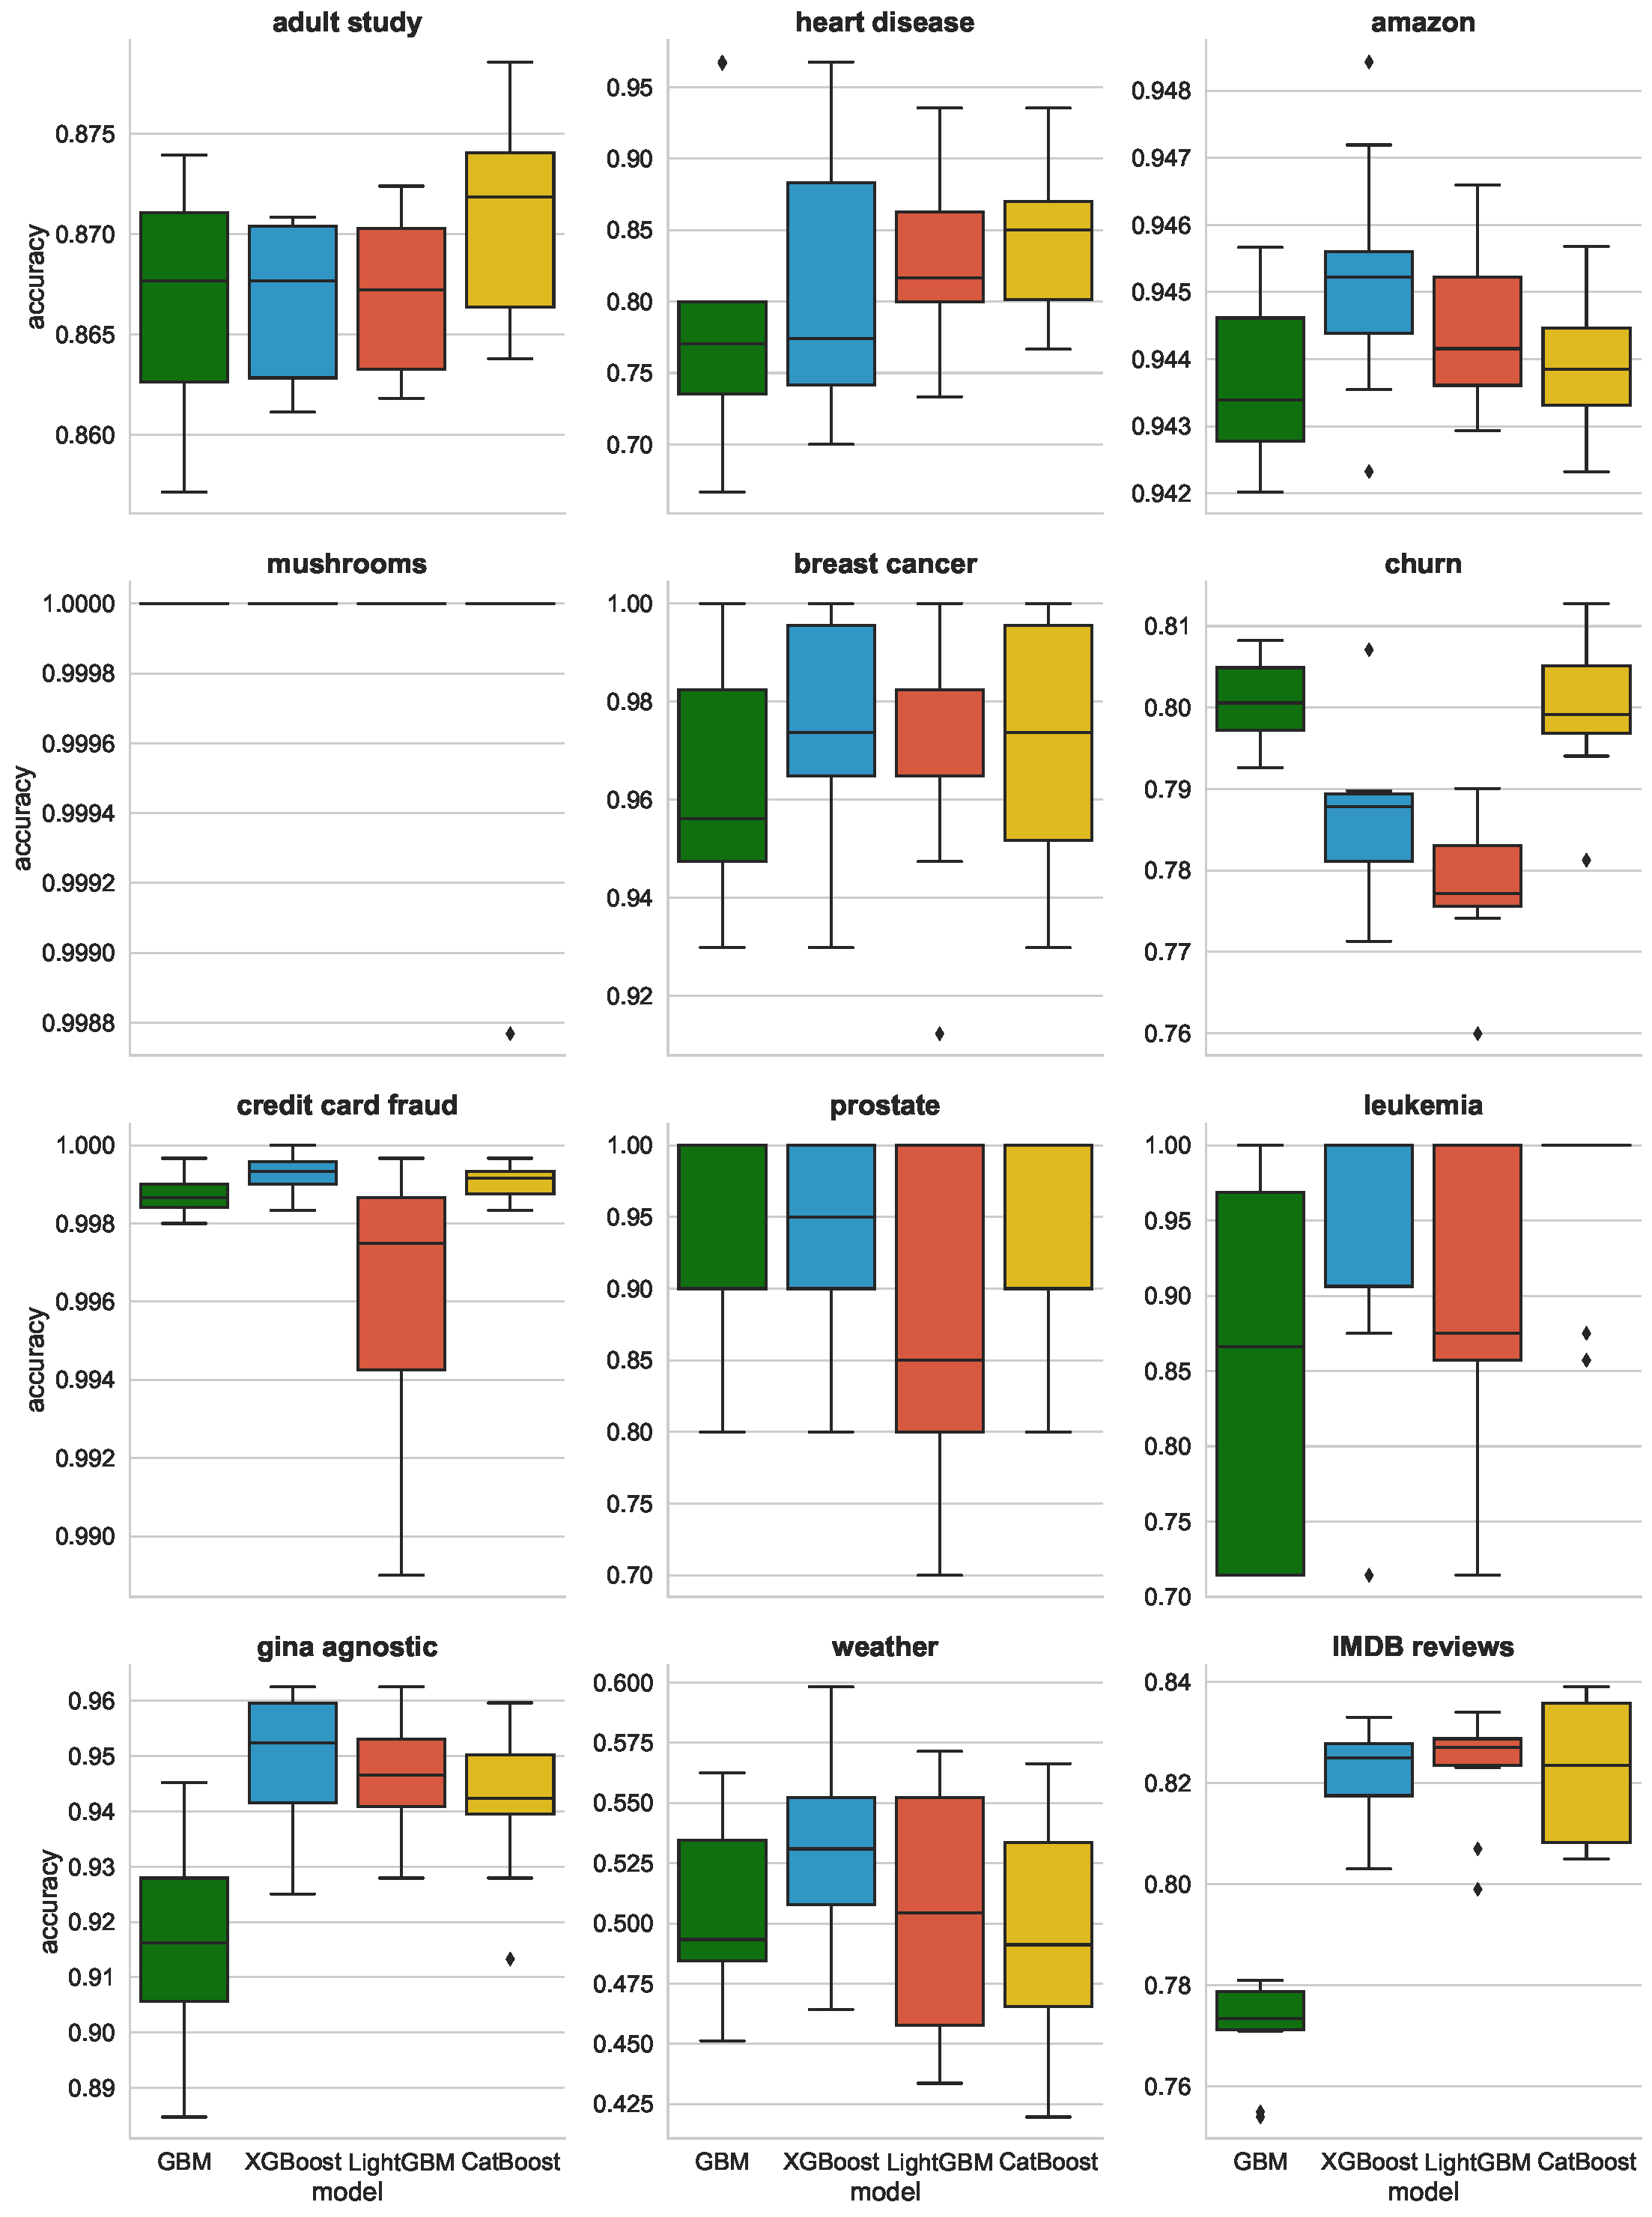
\includegraphics{plots/results_accuracy_12_datasets_no_tuning_150_50_trees_facet.pdf}}
	\caption{Accuracy distributions across 12 datasets without hyperparameter tuning}
	\label{fig:no_tuning_accuracy}
\end{figure}

Performance of each of the GBM implementation varies a lot when considering different datasets. There is no algorithm which would perform the best across all datasets, however, it can be observed that GBM proposed by Friedman \cite{friedman_gbm} almost always performs the worst (except for \emph{churn} and \emph{credit card fraud} datasets). Baseline versions of XGBoost and CatBoost seem to perform the best in terms of accuracy.

The corresponding distributions of performance measures can be summarized by their mean and standard deviation --- an overview has been presented in Table~\ref{tab:no_tuning_accuracy}.

\begin{table}[h!]
\centering
\begin{tabular}{|c|c|c|c|c|}
\hline
\textbf{dataset}  & \textbf{GBM}  & \textbf{XGBoost}  & \textbf{LightGBM}  & \textbf{CatBoost} \\ \hline
adult study & \cellcolor{red}0.867 $\pm$ 0.005 & 0.867 $\pm$ 0.004 & 0.867 $\pm$ 0.004 & \cellcolor{green}0.871 $\pm$ 0.005\\ \hline
heart disease &\cellcolor{red} 0.792 $\pm$ 0.101 & 0.808 $\pm$ 0.088 & 0.828 $\pm$ 0.061 & \cellcolor{green}0.841 $\pm$ 0.056\\ \hline
amazon & \cellcolor{red}0.944 $\pm$ 0.001 & \cellcolor{green}0.945 $\pm$ 0.002 & \cellcolor{red}0.944 $\pm$ 0.001 & \cellcolor{red}0.944 $\pm$ 0.001\\ \hline
mushrooms & 1.0 $\pm$ 0.0 & 1.0 $\pm$ 0.0 & 1.0 $\pm$ 0.0 & 1.0 $\pm$ 0.0\\ \hline
breast cancer & \cellcolor{red}0.963 $\pm$ 0.023 & \cellcolor{green}0.974 $\pm$ 0.024 & 0.967 $\pm$ 0.024 & 0.97 $\pm$ 0.027\\ \hline
churn & \cellcolor{green}0.801 $\pm$ 0.005 & 0.786 $\pm$ 0.01 & \cellcolor{red}0.778 $\pm$ 0.008 & 0.8 $\pm$ 0.009\\ \hline
credit card fraud & 0.999 $\pm$ 0.001 & \cellcolor{green}0.999 $\pm$ 0.0 & \cellcolor{red}0.996 $\pm$ 0.003 & \cellcolor{green}0.999 $\pm$ 0.0\\ \hline
prostate & 0.92 $\pm$ 0.079 & 0.94 $\pm$ 0.07 & \cellcolor{red}0.88 $\pm$ 0.114 & \cellcolor{green}0.95 $\pm$ 0.071\\ \hline
leukemia & \cellcolor{red}0.846 $\pm$ 0.126 & 0.946 $\pm$ 0.097 & 0.904 $\pm$ 0.095 & \cellcolor{green}0.973 $\pm$ 0.057\\ \hline
gina agnostic & \cellcolor{red}0.917 $\pm$ 0.019 & \cellcolor{green}0.949 $\pm$ 0.013 & 0.947 $\pm$ 0.01 & 0.941 $\pm$ 0.013\\ \hline
weather & 0.505 $\pm$ 0.038 & \cellcolor{green}0.53 $\pm$ 0.04 & 0.504 $\pm$ 0.052 & \cellcolor{red}0.495 $\pm$ 0.047\\ \hline
IMDB reviews & \cellcolor{red}0.772 $\pm$ 0.01 & 0.822 $\pm$ 0.01 & \cellcolor{green}0.823 $\pm$ 0.011 & 0.822 $\pm$ 0.014\\ \hline
\end{tabular}
\caption{Means and standard deviations of accuracy distributions presented in Figure~\ref{fig:no_tuning_accuracy}}
\label{tab:no_tuning_accuracy}
\end{table}

For each dataset, the best performing models have been marked with green color while the worst ones have been marked with red. Values of mean and standard deviation presented in Table~\ref{tab:no_tuning_accuracy} suggest that indeed baseline versions of XGBoost and CatBoost perform the best --- authors of corresponding implementations \cite{xgboost}, \cite{catboost} most likely put a lot of effort into choosing the best combination of default hyperparameters. On the other hand, GBM and LightGBM tend to perform the worst; for both of them, in some cases the standard deviations of accuracy are quite big, which indicate that baseline versions of GBM and LightGBM do not generalize as well as XGBoost and CatBoost. There are two possible causes which can explain the instability of the results: firstly, GBM lacks L1 and L2 regularization and in the case of LightGBM, values of aforementioned regularization are set to zero by default. For XGBoost and CatBoost, the default value of $\lambda$ used in L2 regularization has been set to 1 and 3, respectively. Secondly, LightGBM uses leaf-wise growth by default, which may lead to overfitting in situation where other hyperparameters are not taken into consideration\footnote{The explanation is provided in LightGBM's documentation: \url{lightgbm.readthedocs.io/en/latest/Parameters-Tuning.html}}.

Similar conclusions can be drawn while analyzing classifiers' performance in terms of F1 score instead of accuracy. However, since AUC takes evaluates models' performance in a different way than accuracy and F1 score, obtained results are quite different --- they have been presented in Figure~\ref{fig:no_tuning_AUC}.

\iffalse
\begin{figure}[H]
	\centering
		\scalebox{0.42}{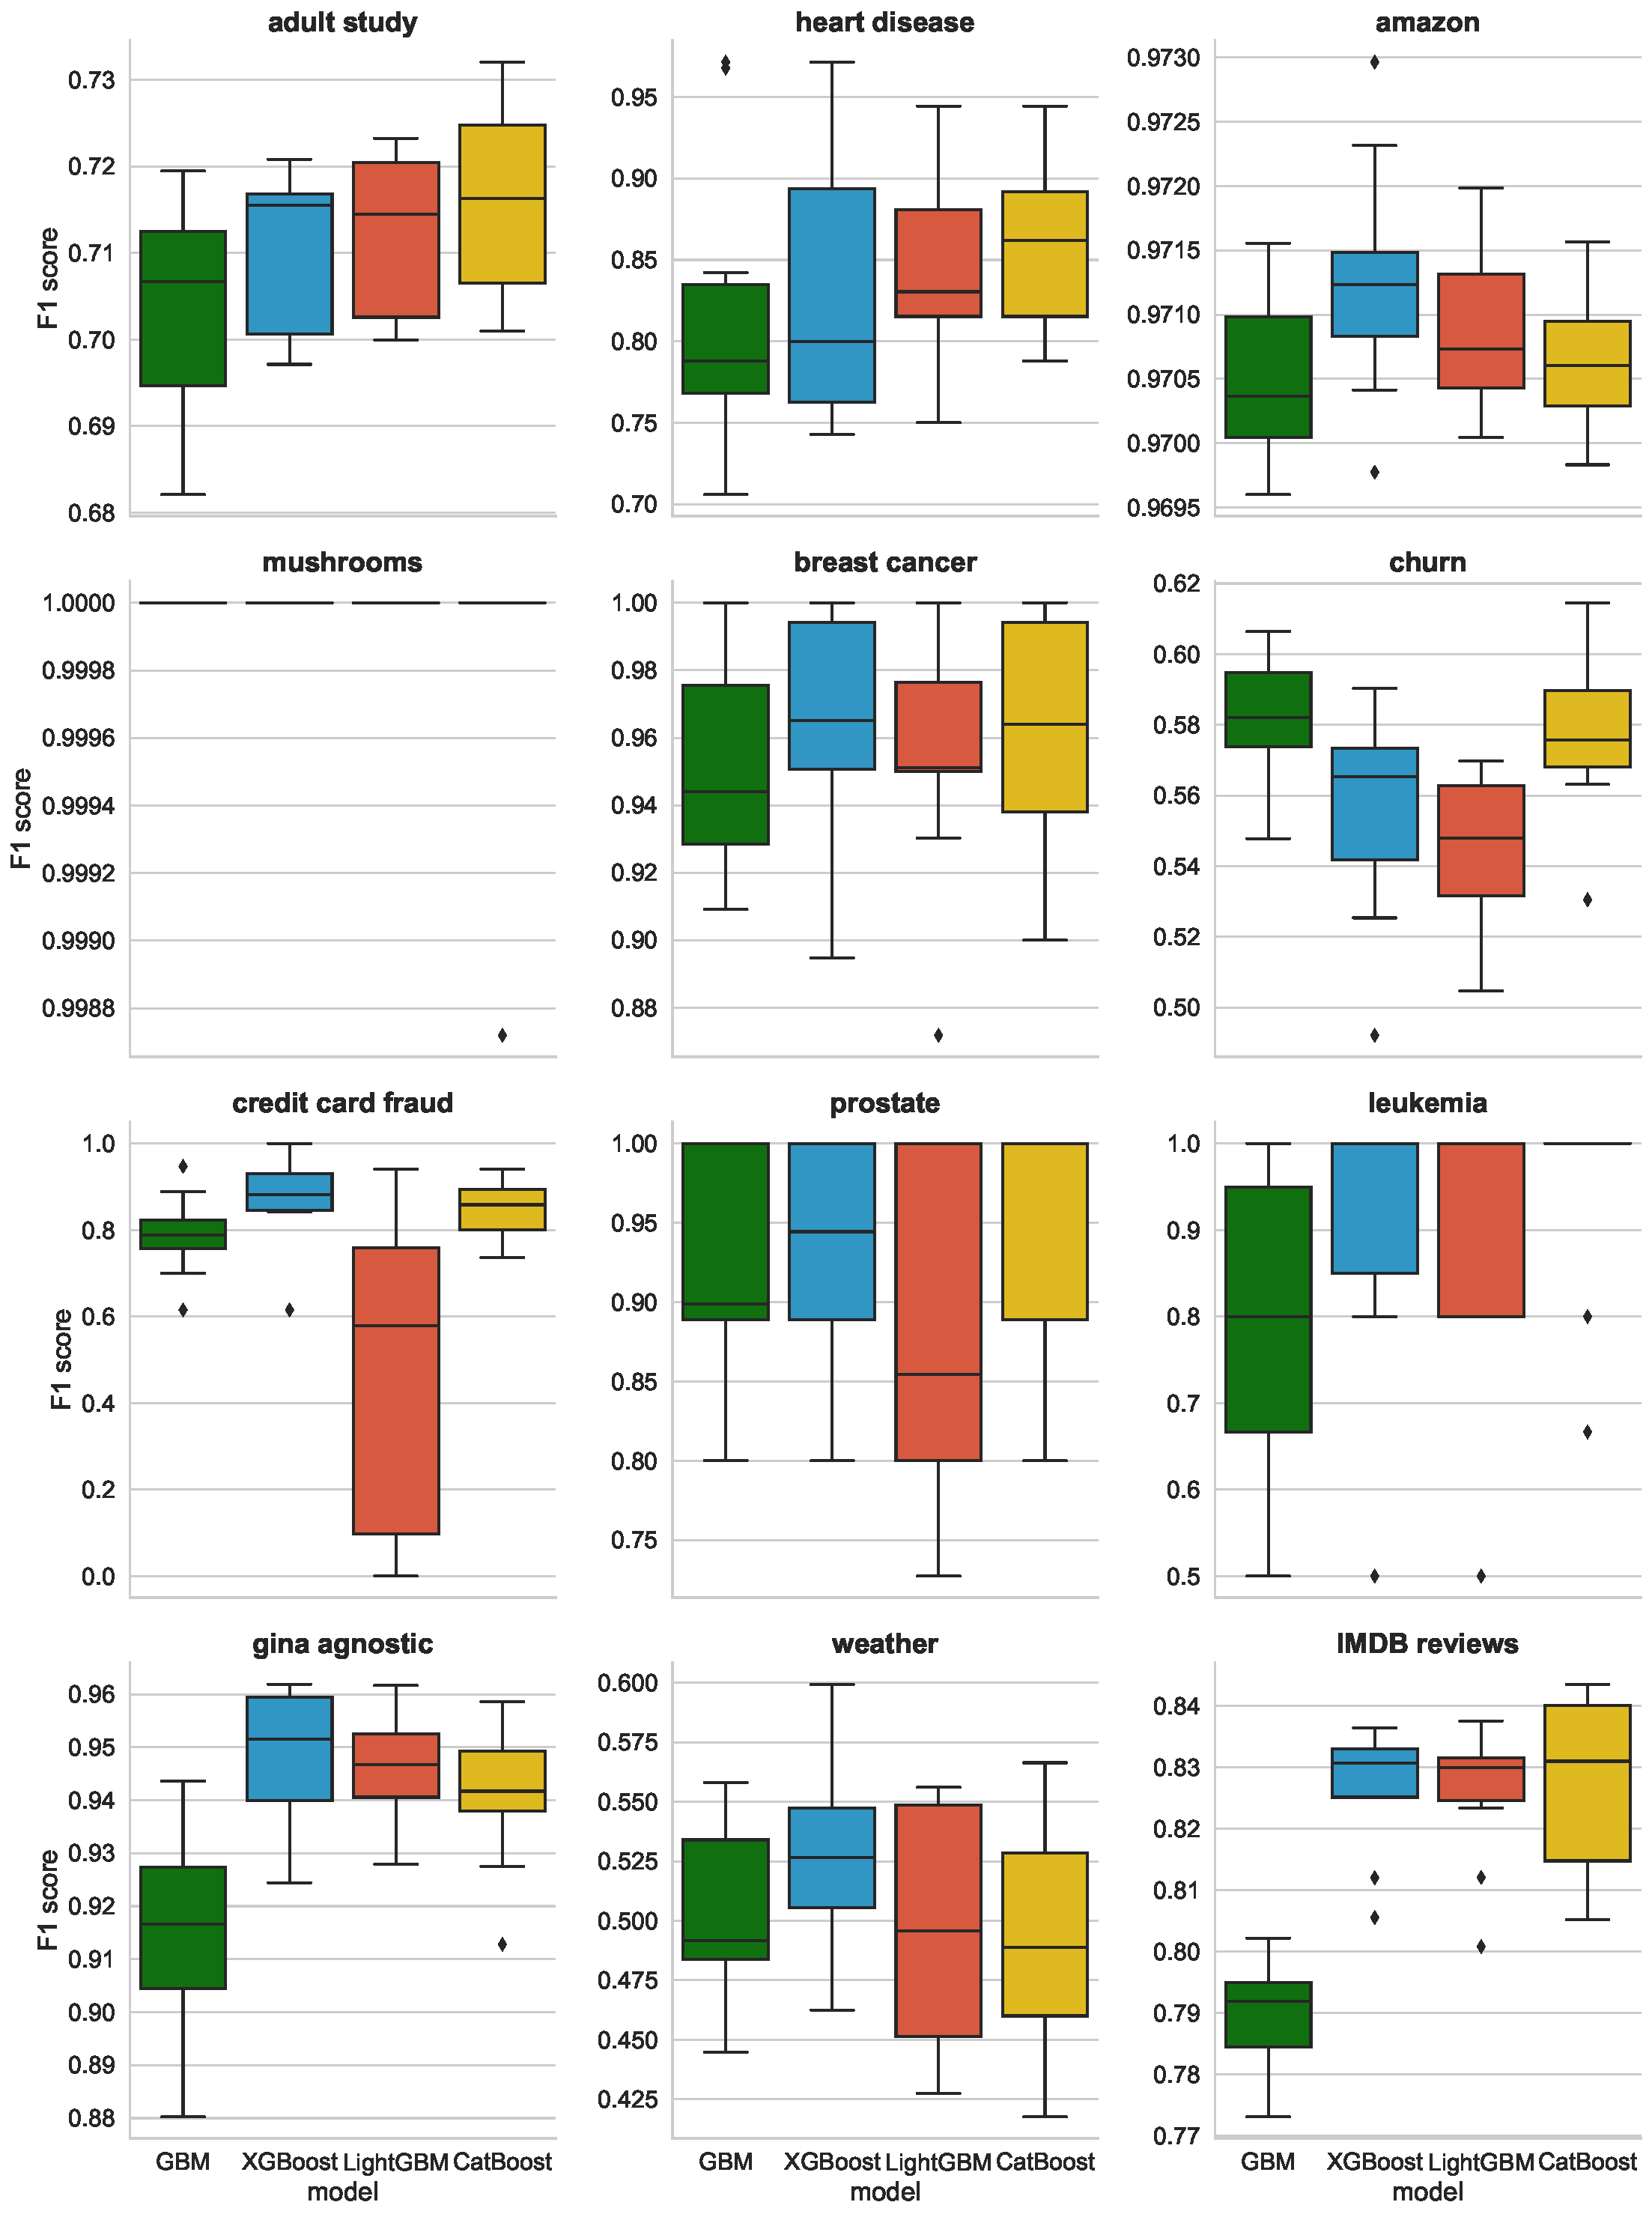
\includegraphics{main/plots/results_f1_score_12_datasets_no_tuning_150_50_trees_facet.pdf}}
	\caption{F1 score distributions across 12 datasets without hyperparameter tuning}
	\label{fig:no_tuning_F1}
\end{figure}
\fi

\begin{figure}[H]
	\centering
		\scalebox{0.42}{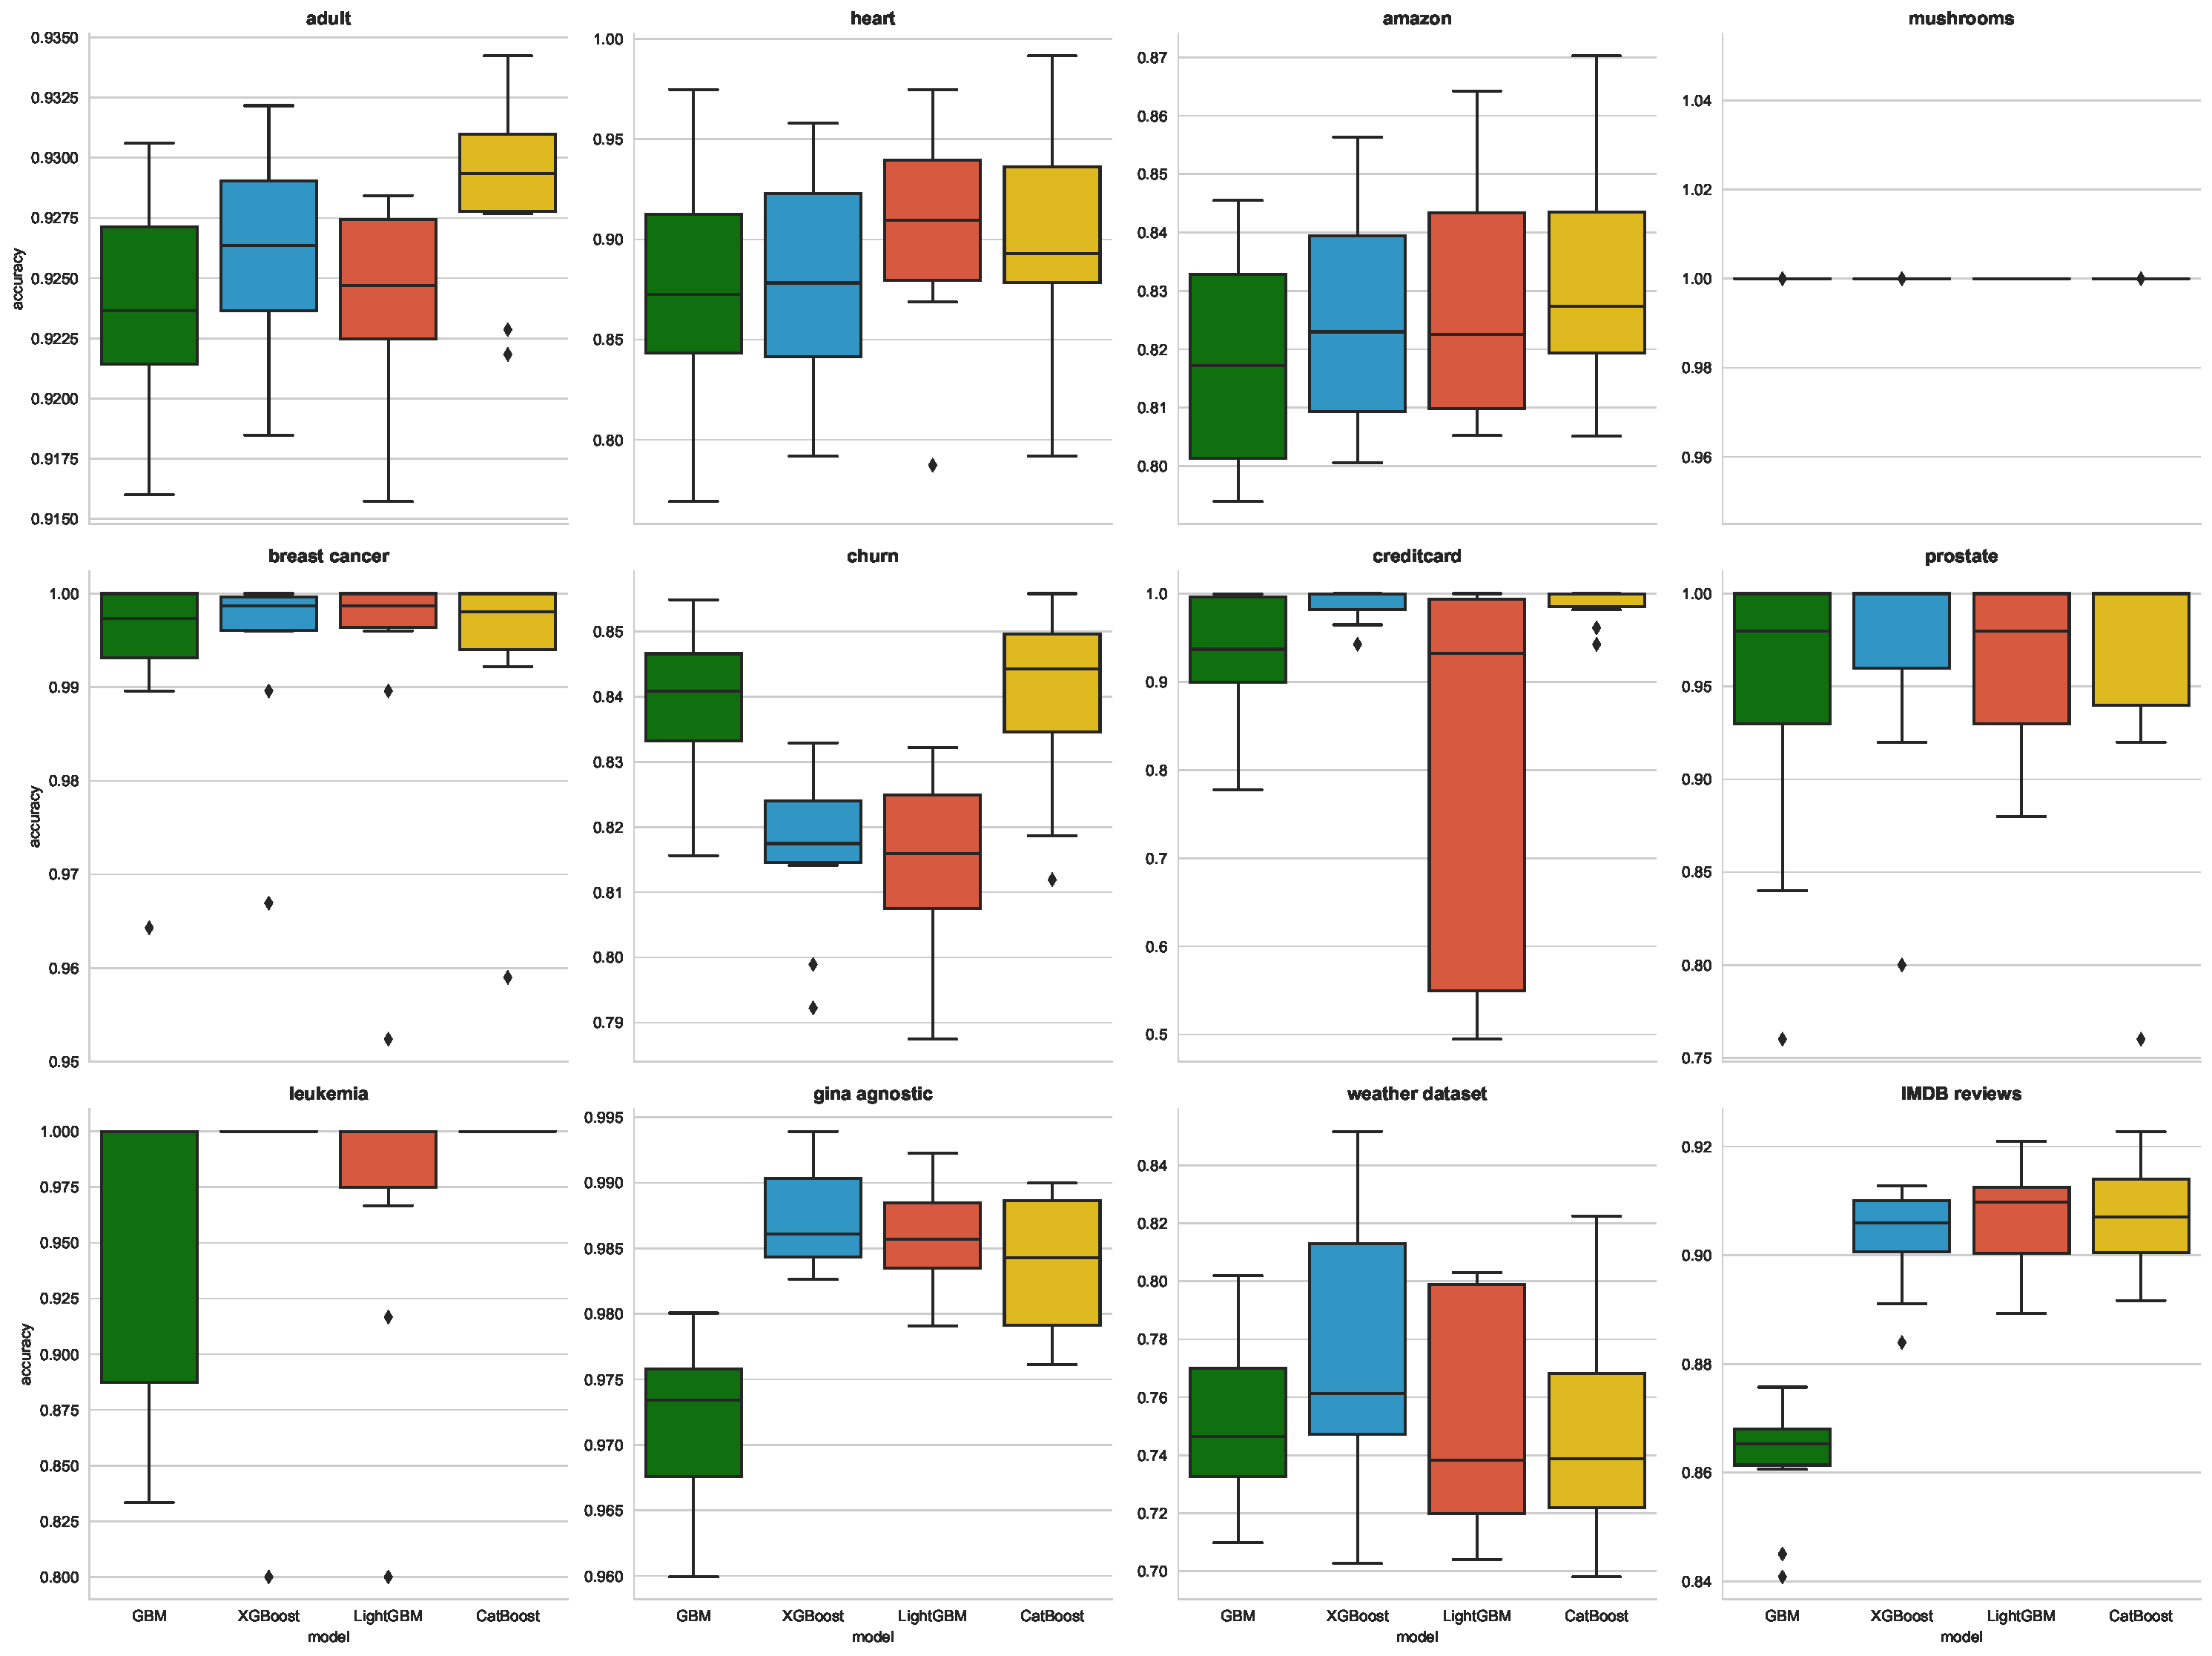
\includegraphics{main/plots/results_AUC_12_datasets_no_tuning_150_50_trees_facet.pdf}}
	\caption{AUC distributions across 12 datasets without hyperparameter tuning}
	\label{fig:no_tuning_AUC}
\end{figure}

In Figure~\ref{fig:no_tuning_AUC} an enormous degradation in terms of AUC in case of LightGBM and the \emph{credit card fraud} dataset can be seen almost immediately. While accuracy (Figure~\ref{fig:no_tuning_accuracy}) ranged from 0.994 to around 0.998, AUC can be as low as 0.55 --- such behaviour is most likely caused by unusual class distribution (to recall, the positive class constitutes only 0.172\% of all labels). On the other hand, AUC seems to vary a lot less compared to accuracy in case of \emph{leukemia} and \emph{prostate} datasets. Numerical summary of AUC scores have been presented in Table~\ref{tab:no_tuning_AUC}.

\begin{table}[h!]
\centering
\begin{tabular}{|c|c|c|c|c|}
\hline
\textbf{dataset}  & \textbf{GBM}  & \textbf{XGBoost}  & \textbf{LightGBM}  & \textbf{CatBoost} \\ \hline
adult study & \cellcolor{red}0.924 $\pm$ 0.005 & 0.926 $\pm$ 0.004 & \cellcolor{red}0.924 $\pm$ 0.005 & \cellcolor{green}0.929 $\pm$ 0.004\\ \hline
heart disease & \cellcolor{red}0.875 $\pm$ 0.064 & 0.878 $\pm$ 0.056 & \cellcolor{green}0.904 $\pm$ 0.053 & 0.9 $\pm$ 0.056\\ \hline
amazon & \cellcolor{red}0.819 $\pm$ 0.019 & 0.825 $\pm$ 0.019 & 0.828 $\pm$ 0.021 & \cellcolor{green}0.832 $\pm$ 0.021\\ \hline
mushrooms & 1.0 $\pm$ 0.0 & 1.0 $\pm$ 0.0 & 1.0 $\pm$ 0.0 & 1.0 $\pm$ 0.0\\ \hline
breast cancer & 0.994 $\pm$ 0.011 & \cellcolor{green}0.994 $\pm$ 0.01 & \cellcolor{red}0.993 $\pm$ 0.015 & 0.994 $\pm$ 0.013\\ \hline
churn & 0.839 $\pm$ 0.012 & 0.817 $\pm$ 0.013 & \cellcolor{red}0.814 $\pm$ 0.014 & \cellcolor{green}0.84 $\pm$ 0.014\\ \hline
credit card fraud & 0.933 $\pm$ 0.071 & \cellcolor{green}0.988 $\pm$ 0.02 & \cellcolor{red}0.803 $\pm$ 0.229 & \cellcolor{green}0.988 $\pm$ 0.02\\ \hline
prostate & \cellcolor{red}0.944 $\pm$ 0.083 & 0.964 $\pm$ 0.064 & \cellcolor{green}0.964 $\pm$ 0.044 & 0.96 $\pm$ 0.078\\ \hline
leukemia & \cellcolor{red}0.952 $\pm$ 0.078 & 0.98 $\pm$ 0.063 & 0.968 $\pm$ 0.065 & \cellcolor{green}1.0 $\pm$ 0.0\\ \hline
gina agnostic & \cellcolor{red}0.972 $\pm$ 0.006 & \cellcolor{green}0.987 $\pm$ 0.004 & 0.986 $\pm$ 0.004 & 0.984 $\pm$ 0.005\\ \hline
weather & 0.751 $\pm$ 0.031 & \cellcolor{green}0.775 $\pm$ 0.046 & 0.753 $\pm$ 0.041 & \cellcolor{red}0.748 $\pm$ 0.039\\ \hline
IMDB reviews & \cellcolor{red}0.862 $\pm$ 0.011 & 0.903 $\pm$ 0.009 & \cellcolor{green}0.907 $\pm$ 0.01 & \cellcolor{green}0.907 $\pm$ 0.01\\ \hline
\end{tabular}
\caption{Means and standard deviations of AUC distributions presented in Figure~\ref{fig:no_tuning_AUC}}
\label{tab:no_tuning_AUC}
\end{table}

Holistically, AUC values across most of the datasets are quite high. AUC values seem to have smaller spread which is indicated by low values of standard deviations, however one has to keep in mind that AUC and accuracy scores cannot be compared directly. What is really interesting is that CatBoost has managed to achieve perfect AUC score on the \emph{leukemia} dataset. Overall, among baseline versions of GBM, XGBoost, LightGBM and CatBoost both XGBoost and CatBoost seem to perform the best it terms of accuracy, F1 score and AUC while GBM's performance is the worst.

On the other hand, accuracy, F1 score and AUC are not the only criteria which are used in this comparative analysis, the runtimes of the algorithms are also crucial --- in case of non-tuned models, times needed to perform model evaluation have been presented in Figure~\ref{fig:no_tuning_runtimes}.

\begin{figure}[H]
	\centering
		\scalebox{0.42}{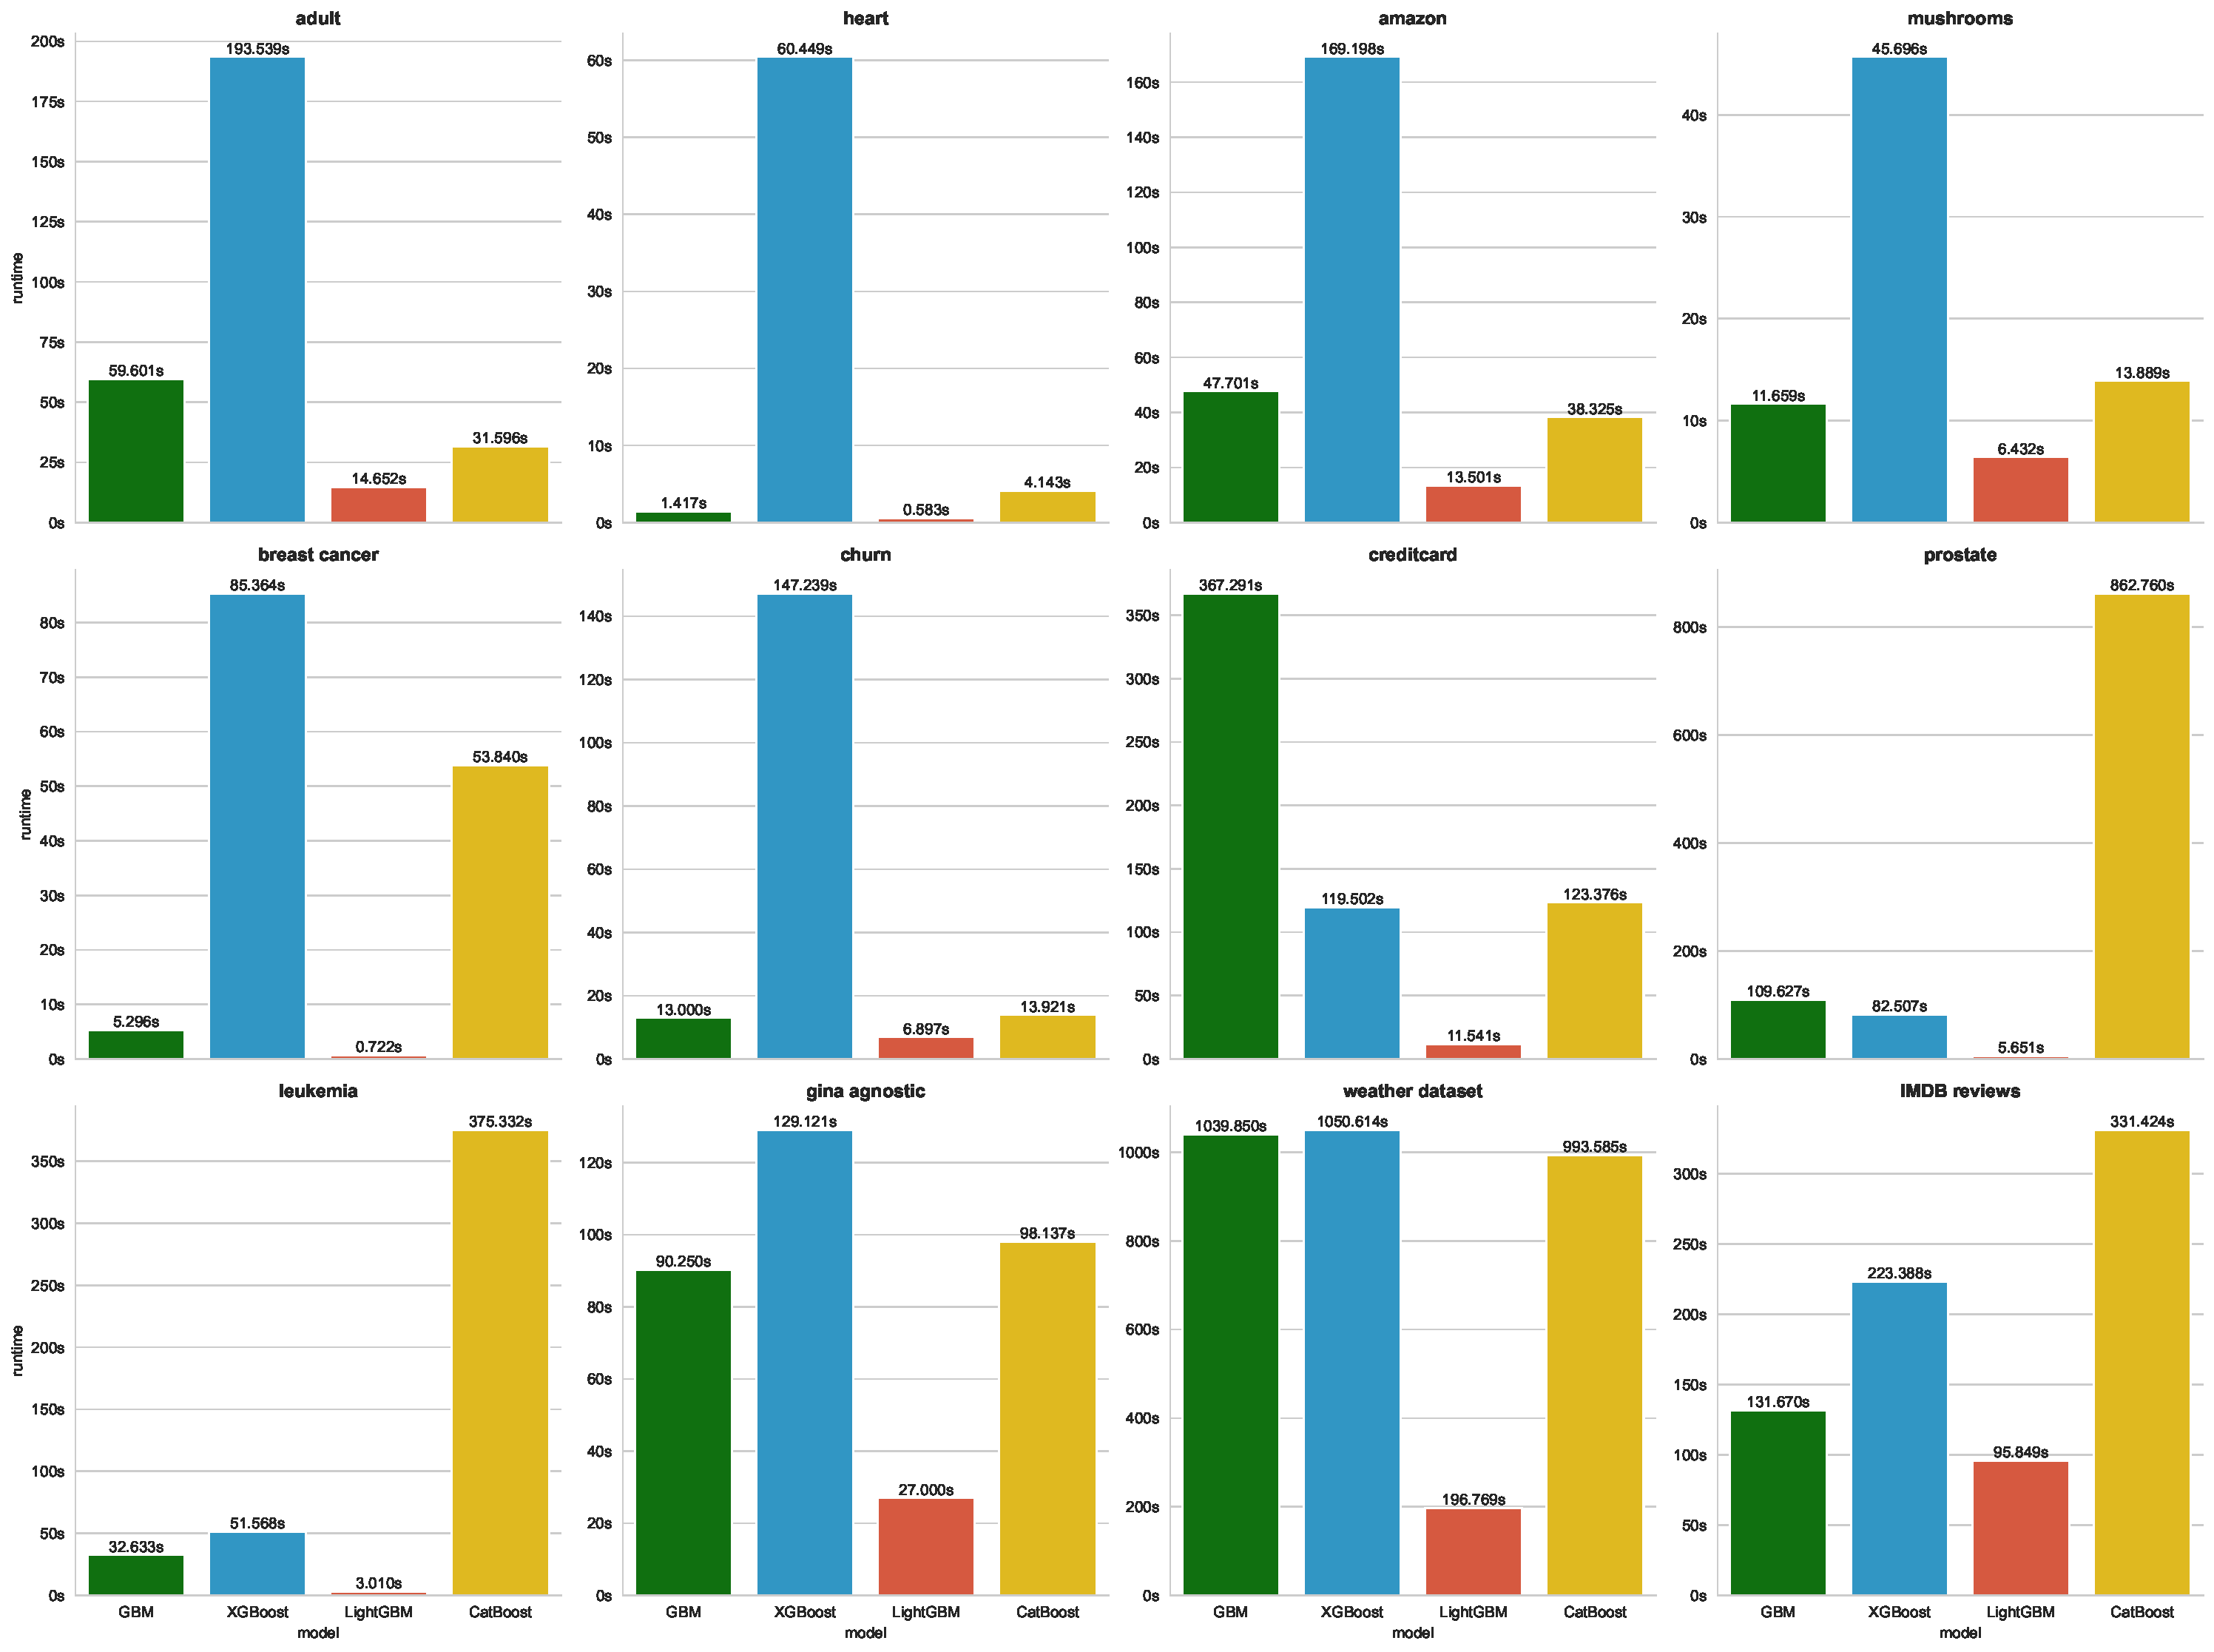
\includegraphics{main/plots/runtimes_12_datasets_no_tuning_150_50_trees_facet.pdf}}
	\caption{Runtimes of the models across 12 datasets without hyperparameter tuning}
	\label{fig:no_tuning_runtimes}
\end{figure}

Overall, the runtimes between models tend to vary a lot less than values of accuracy, F1 score or AUC. However, the models with the best evaluation metrics, namely XGBoost and CatBoost tend to be slower than GBM and much slower than LightGBM. In the case of the first six datasets presented in Table~\ref{tab:datasets}: \emph{adult study}, \emph{heart disease}, \emph{amazon}, \emph{mushrooms}, \emph{breast cancer} and \emph{churn} XGBoost is clearly the slowest. Aforementioned datasets vary greatly in the number of samples (\emph{adult study} has 48842 while \emph{heart disease} contains information about 303 instances), so the length of the datasets clearly had no impact on XGBoost's performance. Additionally, they contain a reasonable number of features (30 at most), so the exact splitting algorithm implemented in XGBoost should still work quite efficiently (even in the case of very highly dimensional data, namely \emph{prostate} and \emph{leukemia} it did well). Thus, the reason behind enormous runtimes of XGBoost on first six datasets presented in Table~\ref{tab:datasets} cannot be uniquely identified.

On the other hand, except for one case (\emph{credit card fraud}) GBM tends to perform rather quickly despite not being computationally optimized like state-of-the-art implementations. LightGBM is consistently the fastest algorithm across all datasets --- histogram-based splitting algorithm, GOSS, EFB and leaf-wise tree growth all contribute to the greatly decreased runtime. Sometimes, LightGBM is faster than competing GBM implementations even by up to two orders of magnitude. It scales very well with high number of samples and very high number of features.

CatBoost's greatest strength lies in datasets with low to moderate number of features (in the case of such datasets XGBoost is surprisingly slow). Great performance in terms of accuracy, F1 score and AUC can be achieved in a very competitive and reasonable amount of time (even despite using Ordered algorithm which is slower than the Plain one). CatBoost scales well with the number of instances, however, it completely cannot handle highly dimensional data (no matter how many training samples are present). Plain version is much slower than other GBM implementations in case of \emph{prostate} and \emph{leukemia} datasets. In case of \emph{gina agnostic} dataset, it is slightly slower than GBM and noticeably faster than XGBoost. In the case of \emph{weather} dataset, Plain CatBoost is almost as slow as XGBoost and CatBoost. Excessive runtimes of CatBoost are surprising, because by default, the value of $\lambda$ responsible for L2 regularization is equal to 3 (to recall, $\lambda=1$ and $\lambda=0$ for XGBoost and LightGBM, respectively).

It has been observed that both Ordered and Plain CatBoost struggle with memory consumption when being used with highly dimensional datasets. Originally, the \emph{weather} dataset contained 4800 features, but Plain CatBoost could not handle that amount of data --- over 17GB of RAM was used, which is quite inefficient (other GBM implementations consumed less than 6GB of RAM). Thus, the size of \emph{weather} dataset had to be reduced to 2500. Such computational infeasibility of CatBoost in unacceptable, especially that it cannot be used with highly dimensional datasets on reasonably new personal computers or laptops (most of them will have up to 16GB of RAM memory).

Friedman test with Nemenyi post hoc analysis has been performed to rank the performance of non-tuned versions of GBM, XGBoost, LightGBM and CatBoost across twelve datasets described in Table~\ref{tab:datasets}. The results in form of a heatmap have been presented in Figure~\ref{fig:no_tuning_accuracy_heatmap}. In each cell two values are displayed: the one in the upper left corner denotes the rank of the model on the left hand side of the heatmap while the other one points at the rank of the model at the bottom.

\begin{figure}[H]
	\centering
		\scalebox{0.7}{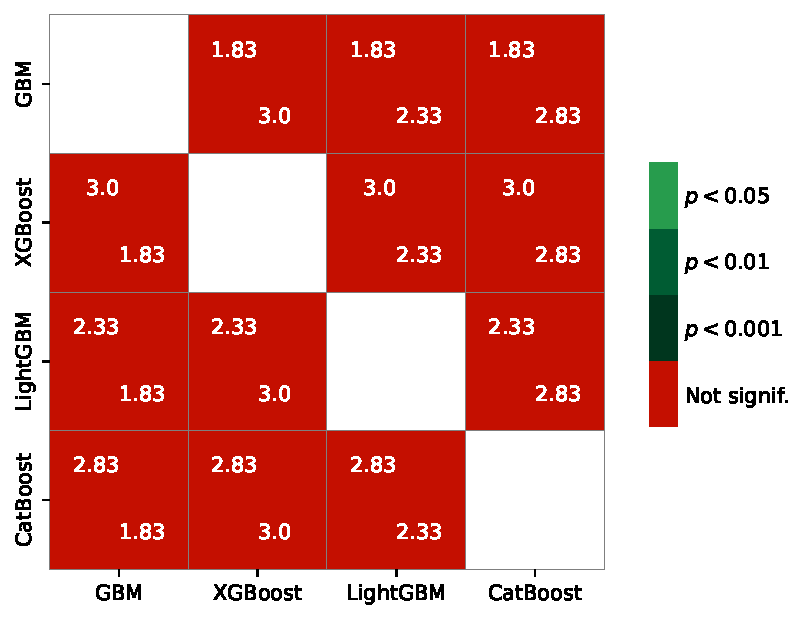
\includegraphics{main/plots/heatmap_accuracy_12_datasets_no_tuning_150_50_trees.pdf}}
	\caption{Ranking of models' accuracy scores. Critical difference $CD = 1.354$}
	\label{fig:no_tuning_accuracy_heatmap}
\end{figure}

The ranking could indicate that XGBoost is the most accurate baseline model. CatBoost's performance is similar, LightGBM and GBM are significantly worse. However, it cannot be explicitly stated that for example XGBoost is a better model than GBM, because the difference in ranks is lower than the Critical difference threshold equal to 1.354. Fortunately, in case of the F1 score XGBoost is in fact better than GBM --- an illustration of the ranking have been presented in Figure~\ref{fig:no_tuning_F1_heatmap}.

\begin{figure}[H]
	\centering
		\scalebox{0.7}{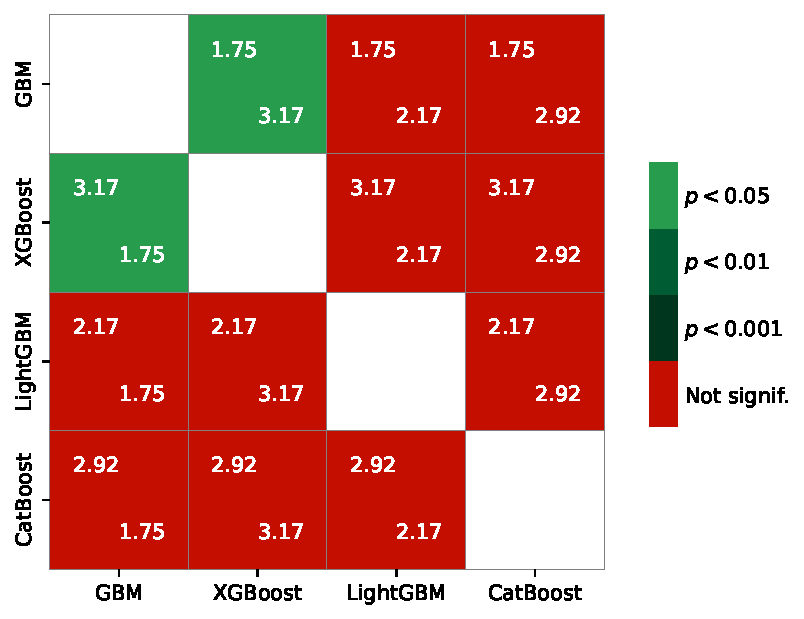
\includegraphics{main/plots/heatmap_f1_score_12_datasets_no_tuning_150_50_trees.pdf}}
	\caption{Ranking of models' F1 scores. Critical difference $CD = 1.354$}
	\label{fig:no_tuning_F1_heatmap}
\end{figure}

In case of F1 score the difference in performance between GBM and XGBoost is bigger; it is also statistically significant. A similar observation can be made in case of AUC score.

\subsection{Analysis of models tuned with Bayesian optimization}\label{section_tpe}
In this section, comparative analysis of GBM, XGBoost, LightGBM and CatBoost models tuned using Tree Parzen Estimators have been carried out. The procedure which has been used for selection of optimal hyperparameters and evaluation of models have been described in Scheme~\ref{eval_scheme}. Due to the sequential nature of Bayesian optimization, the number of tuning iterations for each of the gradient boosting implementation has been set to 15 (by default, only 10 iterations are performed).

One of the aims of model selection in form of hyperparameter tuning is to find models with the best performance possible. Thus, it is absolutely essential to define a set of initial hyperparameters (further referred as \emph{init}) and a search space which will be used in the tuning. To preserve consistency with the experiment described in Section~\ref{section:baseline}, the number of trees and \emph{boosting\_type} in case of LightGBM and CatBoost remain unchanged. Following the advice given in \cite{comparative_analysis} and in \cite{friedman_gbm}, the number of trees has been fixed to the highest computationally feasible value (to recall, it is equal to 150 except for \emph{gina agnostic}, \emph{weather} and \emph{IMDB reviews} datasets where it has been set to 50) and consequently \emph{learning\_rate} will be one of the tuned hyperparameters.

In case of other hyperparameters used in \emph{init} and tuning, an extensive study of each of the GBM implementations' documentation has been carried out. Documentations greatly vary in lengths: GBM\footnote{\url{scikit-learn.org/stable/modules/generated/sklearn.ensemble.GradientBoostingClassifier}} has the shortest one, followed by CatBoost\footnote{\url{catboost.ai/en/docs/references/training-parameters/}}; XGBoost\footnote{\url{xgboost.readthedocs.io/en/stable/parameter.html}} and LightGBM\footnote{\url{lightgbm.readthedocs.io/en/latest/Parameters.html}} in particular provide the most exhaustive documentations, because their implementations \cite{xgboost}, \cite{lightgbm} contain the biggest number of available hyperparameters. Additionally, Friedman's advice regarding stochastic gradient boosting \cite{friedman_stoch} has been considered, as well as the choice of hyperparameters and search spaces which were described in \cite{catboost}, \cite{comparative_analysis} and \cite{competitive_analysis}. The conclusions from the studied documentations and literature suggest the following:
\begin{enumerate}
    \item As it has been stated before, the number of trees has been fixed, but \emph{learning\_rate} is tuned.
    \item In conjunction with the advice given in \cite{friedman_stoch} and \cite{comparative_analysis}, instances and features subsampling have been set to fixed values; it is not worth to tune them. Also, \emph{subsample} cannot be used in case of LightGBM since GOSS mode is used.
    \item In \cite{catboost}, \cite{comparative_analysis} and \cite{competitive_analysis} the maximum depth of a tree (or number of leaves in case of LightGBM), L1 and L2 regularization were common hyperparameters which were tuned, so in this work they will also be a part of the search spaces.
    \item Also, algorithm-specific hyperparameters are a common choice during the process of model selection, thus they will also be considered. These include: XGBoost's \emph{gamma}, LightGBM's \emph{top\_rate} and \emph{other\_rate} and CatBoost's \emph{leaf\_estimation\_iterations}.
\end{enumerate}

Additionally, some \emph{init} hyperparameters as well as some search spaces are different in case of various datasets. For those with a small number of samples, \emph{subsample} fraction has been set to 1 --- excessive subsampling of a dataset which is already small can lead to a degradation of performance. Moreover, upper bound of regularization strength in search spaces has been increased in datasets with very high number of features.

The summary of initial hyperparametrization as well as search spaces has been presented in Table~\ref{tab:init_tuning}. In search spaces, discrete values in square brackets are sampled uniformly, while continuous ones are sampled either from uniform ($\mathcal{U}$) or log-uniform ($\log\mathcal{U}$) distributions.

\begin{landscape}
\begin{table}[]
\centering
\resizebox{670pt}{!}{%
\begin{tabular}{ccccc}
\hline
\multicolumn{1}{|c|}{\textbf{datasets}} &
  \multicolumn{1}{c|}{\textbf{\begin{tabular}[c]{@{}c@{}}GBM\\ init\end{tabular}}} &
  \multicolumn{1}{c|}{\textbf{\begin{tabular}[c]{@{}c@{}}XGBoost\\ init\end{tabular}}} &
  \multicolumn{1}{c|}{\textbf{\begin{tabular}[c]{@{}c@{}}LightGBM\\ init\end{tabular}}} &
  \multicolumn{1}{c|}{\textbf{\begin{tabular}[c]{@{}c@{}}CatBoost\\ init\end{tabular}}} \\ \hline
\multicolumn{1}{|c|}{\begin{tabular}[c]{@{}c@{}}adult study\\ amazon\\ mushrooms\\ churn\\ credit card fraud\end{tabular}} &
  \multicolumn{1}{c|}{\begin{tabular}[c]{@{}c@{}}n\_estimators: 150\\ subsample: 0.75\\ max\_features: 0.6\end{tabular}} &
  \multicolumn{1}{c|}{\begin{tabular}[c]{@{}c@{}}n\_estimators: 150\\ subsample: 0.75\\ colsample\_bynode: 0.6\end{tabular}} &
  \multicolumn{1}{c|}{\begin{tabular}[c]{@{}c@{}}boosting\_type: "goss"\\ n\_estimators: 150\\ colsample\_bynode: 0.6\end{tabular}} &
  \multicolumn{1}{c|}{\begin{tabular}[c]{@{}c@{}}boosting\_type: "Ordered"\\ n\_estimators: 150\\ subsample: 0.75\\ colsample\_bylevel: 0.6\end{tabular}} \\ \hline
\multicolumn{1}{|c|}{\begin{tabular}[c]{@{}c@{}}heart disease\\ breast cancer\end{tabular}} &
  \multicolumn{1}{c|}{\begin{tabular}[c]{@{}c@{}}Same as above,\\  but with subsample = 1\end{tabular}} &
  \multicolumn{1}{c|}{\begin{tabular}[c]{@{}c@{}}Same as above,\\  but with subsample = 1\end{tabular}} &
  \multicolumn{1}{c|}{\begin{tabular}[c]{@{}c@{}}Same as above\end{tabular}} &
  \multicolumn{1}{c|}{\begin{tabular}[c]{@{}c@{}}Same as above,\\  but with subsample = 1\end{tabular}} \\ \hline
\multicolumn{1}{|c|}{\begin{tabular}[c]{@{}c@{}}prostate\\ leukemia\end{tabular}} &
  \multicolumn{1}{c|}{\begin{tabular}[c]{@{}c@{}}n\_estimators: 150\\ subsample: 1\\ max\_features: 0.4\end{tabular}} &
  \multicolumn{1}{c|}{\begin{tabular}[c]{@{}c@{}}n\_estimators: 150\\ subsample: 1\\ colsample\_bynode: 0.4\end{tabular}} &
  \multicolumn{1}{c|}{\begin{tabular}[c]{@{}c@{}}boosting\_type: "goss"\\ n\_estimators: 150\\ colsample\_bynode: 0.4\end{tabular}} &
  \multicolumn{1}{c|}{\begin{tabular}[c]{@{}c@{}}boosting\_type: "Plain"\\ n\_estimators: 150\\ subsample: 1\\ colsample\_bylevel: 0.4\end{tabular}} \\ \hline
\multicolumn{1}{|c|}{\begin{tabular}[c]{@{}c@{}}gina agnostic\\ weather\\ IMDB reviews\end{tabular}} &
  \multicolumn{1}{c|}{\begin{tabular}[c]{@{}c@{}}n\_estimators: 50\\ subsample: 0.5\\ max\_features: 0.4\end{tabular}} &
  \multicolumn{1}{c|}{\begin{tabular}[c]{@{}c@{}}n\_estimators: 50\\ subsample: 0.5\\ colsample\_bynode: 0.4\end{tabular}} &
  \multicolumn{1}{c|}{\begin{tabular}[c]{@{}c@{}}boosting\_type: "goss"\\ n\_estimators: 50\\ colsample\_bynode: 0.4\end{tabular}} &
  \multicolumn{1}{c|}{\begin{tabular}[c]{@{}c@{}}boosting\_type: "Plain"\\ n\_estimators: 50\\ subsample: 0.5\\ colsample\_bylevel: 0.4\end{tabular}} \\ \hline
 &
   &
   &
   &
   \\ \hline
\multicolumn{1}{|c|}{\textbf{datasets}} &
  \multicolumn{1}{c|}{\textbf{\begin{tabular}[c]{@{}c@{}}GBM\\ tuning\end{tabular}}} &
  \multicolumn{1}{c|}{\textbf{\begin{tabular}[c]{@{}c@{}}XGBoost\\ tuning\end{tabular}}} &
  \multicolumn{1}{c|}{\textbf{\begin{tabular}[c]{@{}c@{}}LightGBM\\ tuning\end{tabular}}} &
  \multicolumn{1}{c|}{\textbf{\begin{tabular}[c]{@{}c@{}}CatBoost\\ tuning\end{tabular}}} \\ \hline
\multicolumn{1}{|c|}{\begin{tabular}[c]{@{}c@{}}adult study\\ amazon\\ mushrooms\\ churn\\ credit card fraud\end{tabular}} &
  \multicolumn{1}{c|}{\begin{tabular}[c]{@{}c@{}}max\_depth: [2, 3, 4, 5, 8, 10]\\ learning\_rate: \logU(0.01, 0.3)\\ min\_samples\_split: [2, 5, 10]\end{tabular}} &
  \multicolumn{1}{c|}{\begin{tabular}[c]{@{}c@{}}max\_depth: [2, 3, 4, 5, 8, 10]\\ learning\_rate: \logU(0.01, 0.3)\\ gamma: \U(0, 3)\\ alpha: \U(0, 1)\\ lambda: \U(0, 3)\end{tabular}} &
  \multicolumn{1}{c|}{\begin{tabular}[c]{@{}c@{}}num\_leaves: [3, 7, 15, 31, 127]\\ learning\_rate: \logU(0.01, 0.3)\\ top\_rate: \U(0.1, 0.5)\\ other\_rate: \U(0.05, 0.2)\\ reg\_alpha: \U(0, 1)\\ reg\_lambda: \U(0, 3)\end{tabular}} &
  \multicolumn{1}{c|}{\begin{tabular}[c]{@{}c@{}}max\_depth: [2, 3, 4, 5, 8, 10]\\ leaf\_estimation\_iterations: [1, 10]\\ l2\_leaf\_reg: \U(0, 5)\end{tabular}} \\ \hline
\multicolumn{1}{|c|}{\begin{tabular}[c]{@{}c@{}}heart disease\\ breast cancer\end{tabular}} &
  \multicolumn{1}{c|}{Same as above} &
  \multicolumn{1}{c|}{Same as above} &
  \multicolumn{1}{c|}{Same as above} &
  \multicolumn{1}{c|}{Same as above} \\ \hline
\multicolumn{1}{|c|}{\begin{tabular}[c]{@{}c@{}}prostate\\ leukemia\end{tabular}} &
  \multicolumn{1}{c|}{\begin{tabular}[c]{@{}c@{}}max\_depth: [2, 3, 4, 5, 8, 10]\\ learning\_rate: \logU(0.01, 0.3)\\ min\_samples\_split: [2, 5, 10]\end{tabular}} &
  \multicolumn{1}{c|}{\begin{tabular}[c]{@{}c@{}}max\_depth: [2, 3, 4, 5, 8, 10]\\ learning\_rate: \logU(0.01, 0.3)\\ gamma: \U(0, 10)\\ alpha: \U(0, 5)\\ lambda: \U(0, 10)\end{tabular}} &
  \multicolumn{1}{c|}{\begin{tabular}[c]{@{}c@{}}num\_leaves: [3, 7, 15, 31, 127]\\ learning\_rate: \logU(0.01, 0.3)\\ top\_rate: \U(0.1, 0.5)\\ other\_rate: \U(0.05, 0.2)\\ reg\_alpha: \U(0, 5)\\ reg\_lambda: \U(0, 10)\end{tabular}} &
  \multicolumn{1}{c|}{\begin{tabular}[c]{@{}c@{}}max\_depth: [2, 3, 4, 5, 8, 10]\\ leaf\_estimation\_iterations: [1, 10]\\ l2\_leaf\_reg: \U(0, 12)\end{tabular}} \\ \hline
\multicolumn{1}{|c|}{\begin{tabular}[c]{@{}c@{}}gina agnostic\\ weather\\ IMDB reviews\end{tabular}} &
  \multicolumn{1}{c|}{Same as above} &
  \multicolumn{1}{c|}{Same as above} &
  \multicolumn{1}{c|}{Same as above} &
  \multicolumn{1}{c|}{Same as above} \\ \hline
\end{tabular}%
}
\caption{Initial hyperparameters and search spaces for GBM, XGBoost, LightGBM and CatBoost}
\label{tab:init_tuning}
\end{table}
\end{landscape}

Results in terms of accuracy have been presented in Figure~\ref{fig:tpe_accuracy}.

\begin{figure}[H]
	\centering
		\scalebox{0.42}{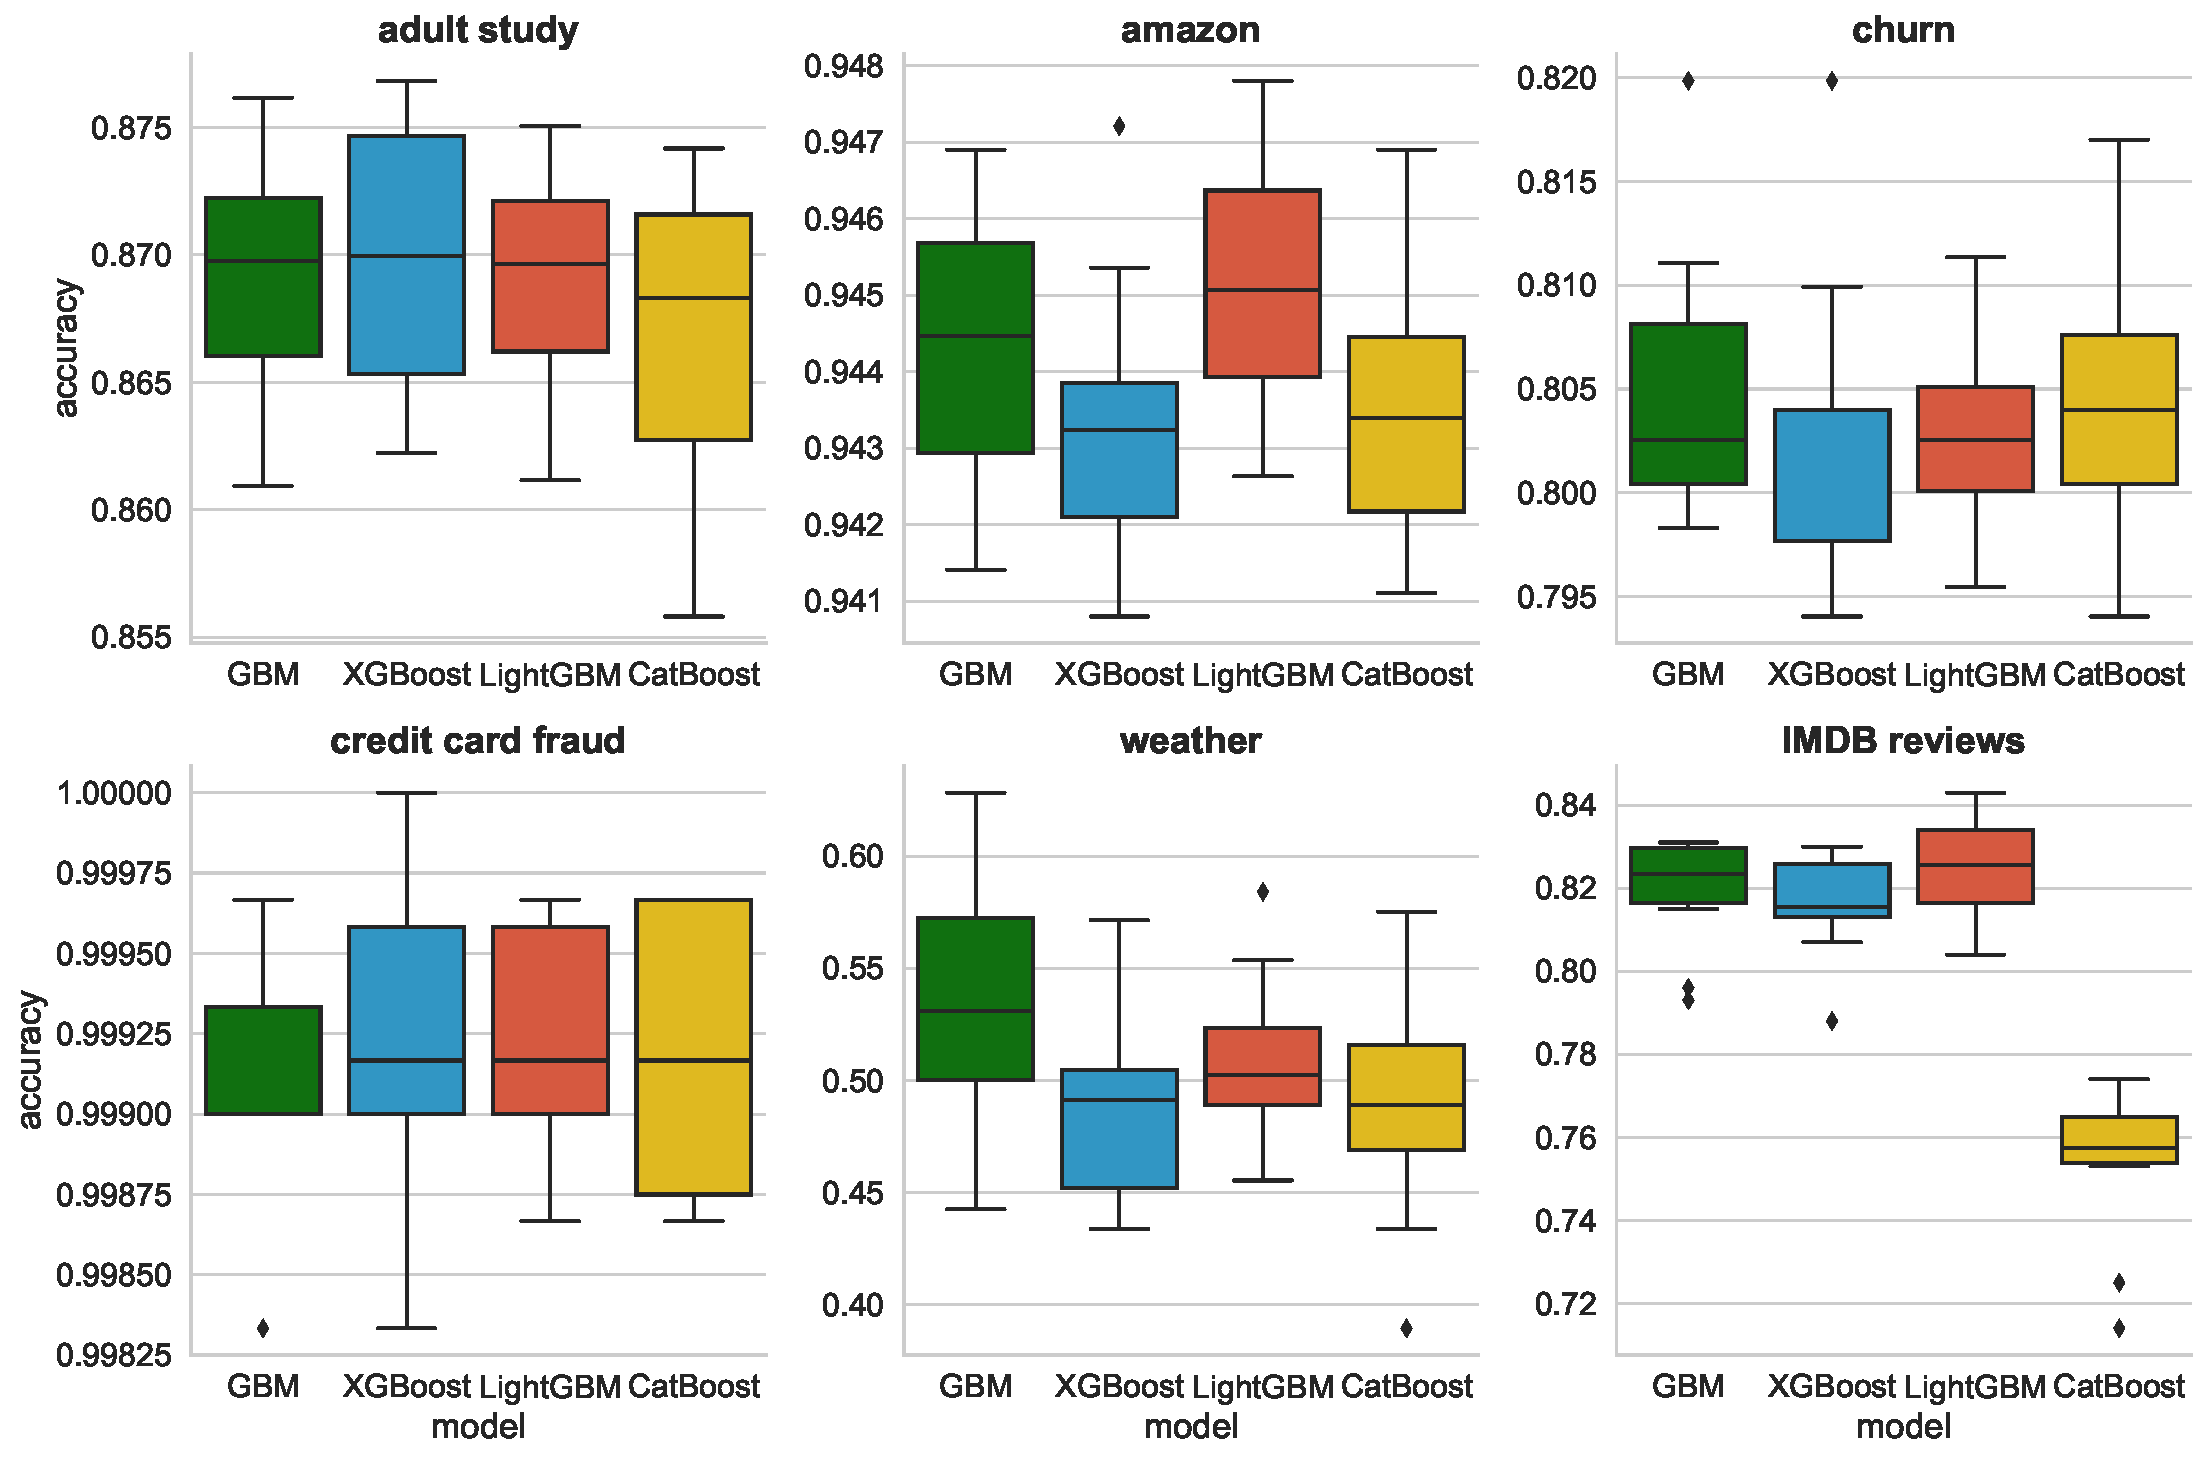
\includegraphics{main/plots/results_accuracy_12_datasets_TPE_150_50_trees_facet.pdf}}
	\caption{Accuracy distributions across 12 datasets with TPE tuning}
	\label{fig:tpe_accuracy}
\end{figure}

Immediately, a vast improvement of gradient boosting and LightGBM can be noticed. Both of the models benefited greatly from hyperparameter tuning and right now all four models: GBM, XGBoost, LightGBM and CatBoost perform very similarly. Moreover, an increase in LightGBM's performance can be observed; corresponding red boxes are much shorter --- it is possible that the inclusion of regularization has resulted in smaller accuracy values. A visual judgment would suggest that among tuned models, LightGBM performs the best. XGBoost is also quite robust, but CatBoost seems to have degraded in performance --- even the original GBM proposed by Friedman in 1999 \cite{friedman_gbm} seems to uniformly outperform it. The means and standard deviations of accuracy distributions for each model and dataset have been presented in Table~\ref{tab:tpe_accuracy}.

\begin{table}[h!]
\centering
\begin{tabular}{|c|c|c|c|c|}
\hline
\textbf{dataset}  & \textbf{GBM}  & \textbf{XGBoost}  & \textbf{LightGBM}  & \textbf{CatBoost} \\ \hline
adult study & 0.869 $\pm$ 0.005 & \cellcolor{green}0.87 $\pm$ 0.006 & 0.869 $\pm$ 0.005 & \cellcolor{red}0.867 $\pm$ 0.006\\ \hline
heart disease & \cellcolor{red}0.815 $\pm$ 0.086 & 0.828 $\pm$ 0.082 & 0.835 $\pm$ 0.061 & \cellcolor{green}0.838 $\pm$ 0.056\\ \hline
amazon & 0.944 $\pm$ 0.002 & \cellcolor{red}0.943 $\pm$ 0.002 & \cellcolor{green}0.945 $\pm$ 0.002 & \cellcolor{red}0.943 $\pm$ 0.002\\ \hline
mushrooms & 1.0 $\pm$ 0.0 & 1.0 $\pm$ 0.0 & 1.0 $\pm$ 0.0 & 1.0 $\pm$ 0.0\\ \hline
breast cancer & \cellcolor{red}0.963 $\pm$ 0.024 & 0.965 $\pm$ 0.023 & 0.97 $\pm$ 0.02 & \cellcolor{green}0.972 $\pm$ 0.03\\ \hline
churn & \cellcolor{green}0.805 $\pm$ 0.007 & \cellcolor{red}0.803 $\pm$ 0.007 & 0.803 $\pm$ 0.004 & 0.804 $\pm$ 0.007\\ \hline
credit card fraud & 0.999 $\pm$ 0.0 & 0.999 $\pm$ 0.0 & 0.999 $\pm$ 0.0 & 0.999 $\pm$ 0.0\\ \hline
prostate & \cellcolor{green}0.95 $\pm$ 0.071 & 0.94 $\pm$ 0.07 & \cellcolor{red}0.94 $\pm$ 0.084 & \cellcolor{green}0.95 $\pm$ 0.071\\ \hline
leukemia & \cellcolor{red}0.918 $\pm$ 0.098 & 0.932 $\pm$ 0.098 & 0.932 $\pm$ 0.098 & \cellcolor{green}0.973 $\pm$ 0.057\\ \hline
gina agnostic & 0.939 $\pm$ 0.012 & 0.937 $\pm$ 0.014 & \cellcolor{green}0.941 $\pm$ 0.014 & \cellcolor{red}0.911 $\pm$ 0.02\\ \hline
weather & \cellcolor{green}0.537 $\pm$ 0.058 & \cellcolor{red}0.486 $\pm$ 0.042 & 0.51 $\pm$ 0.037 & 0.491 $\pm$ 0.055\\ \hline
IMDB reviews & 0.819 $\pm$ 0.014 & 0.816 $\pm$ 0.013 & \cellcolor{green}0.825 $\pm$ 0.013 & \cellcolor{red}0.753 $\pm$ 0.019\\ \hline
\end{tabular}
\caption{Means and standard deviations of accuracy distributions presented in Figure~\ref{fig:tpe_accuracy}}
\label{tab:tpe_accuracy}
\end{table}

The results in case of AUC have been presented in Figure~\ref{fig:tpe_AUC}.

\begin{figure}[H]
	\centering
		\scalebox{0.42}{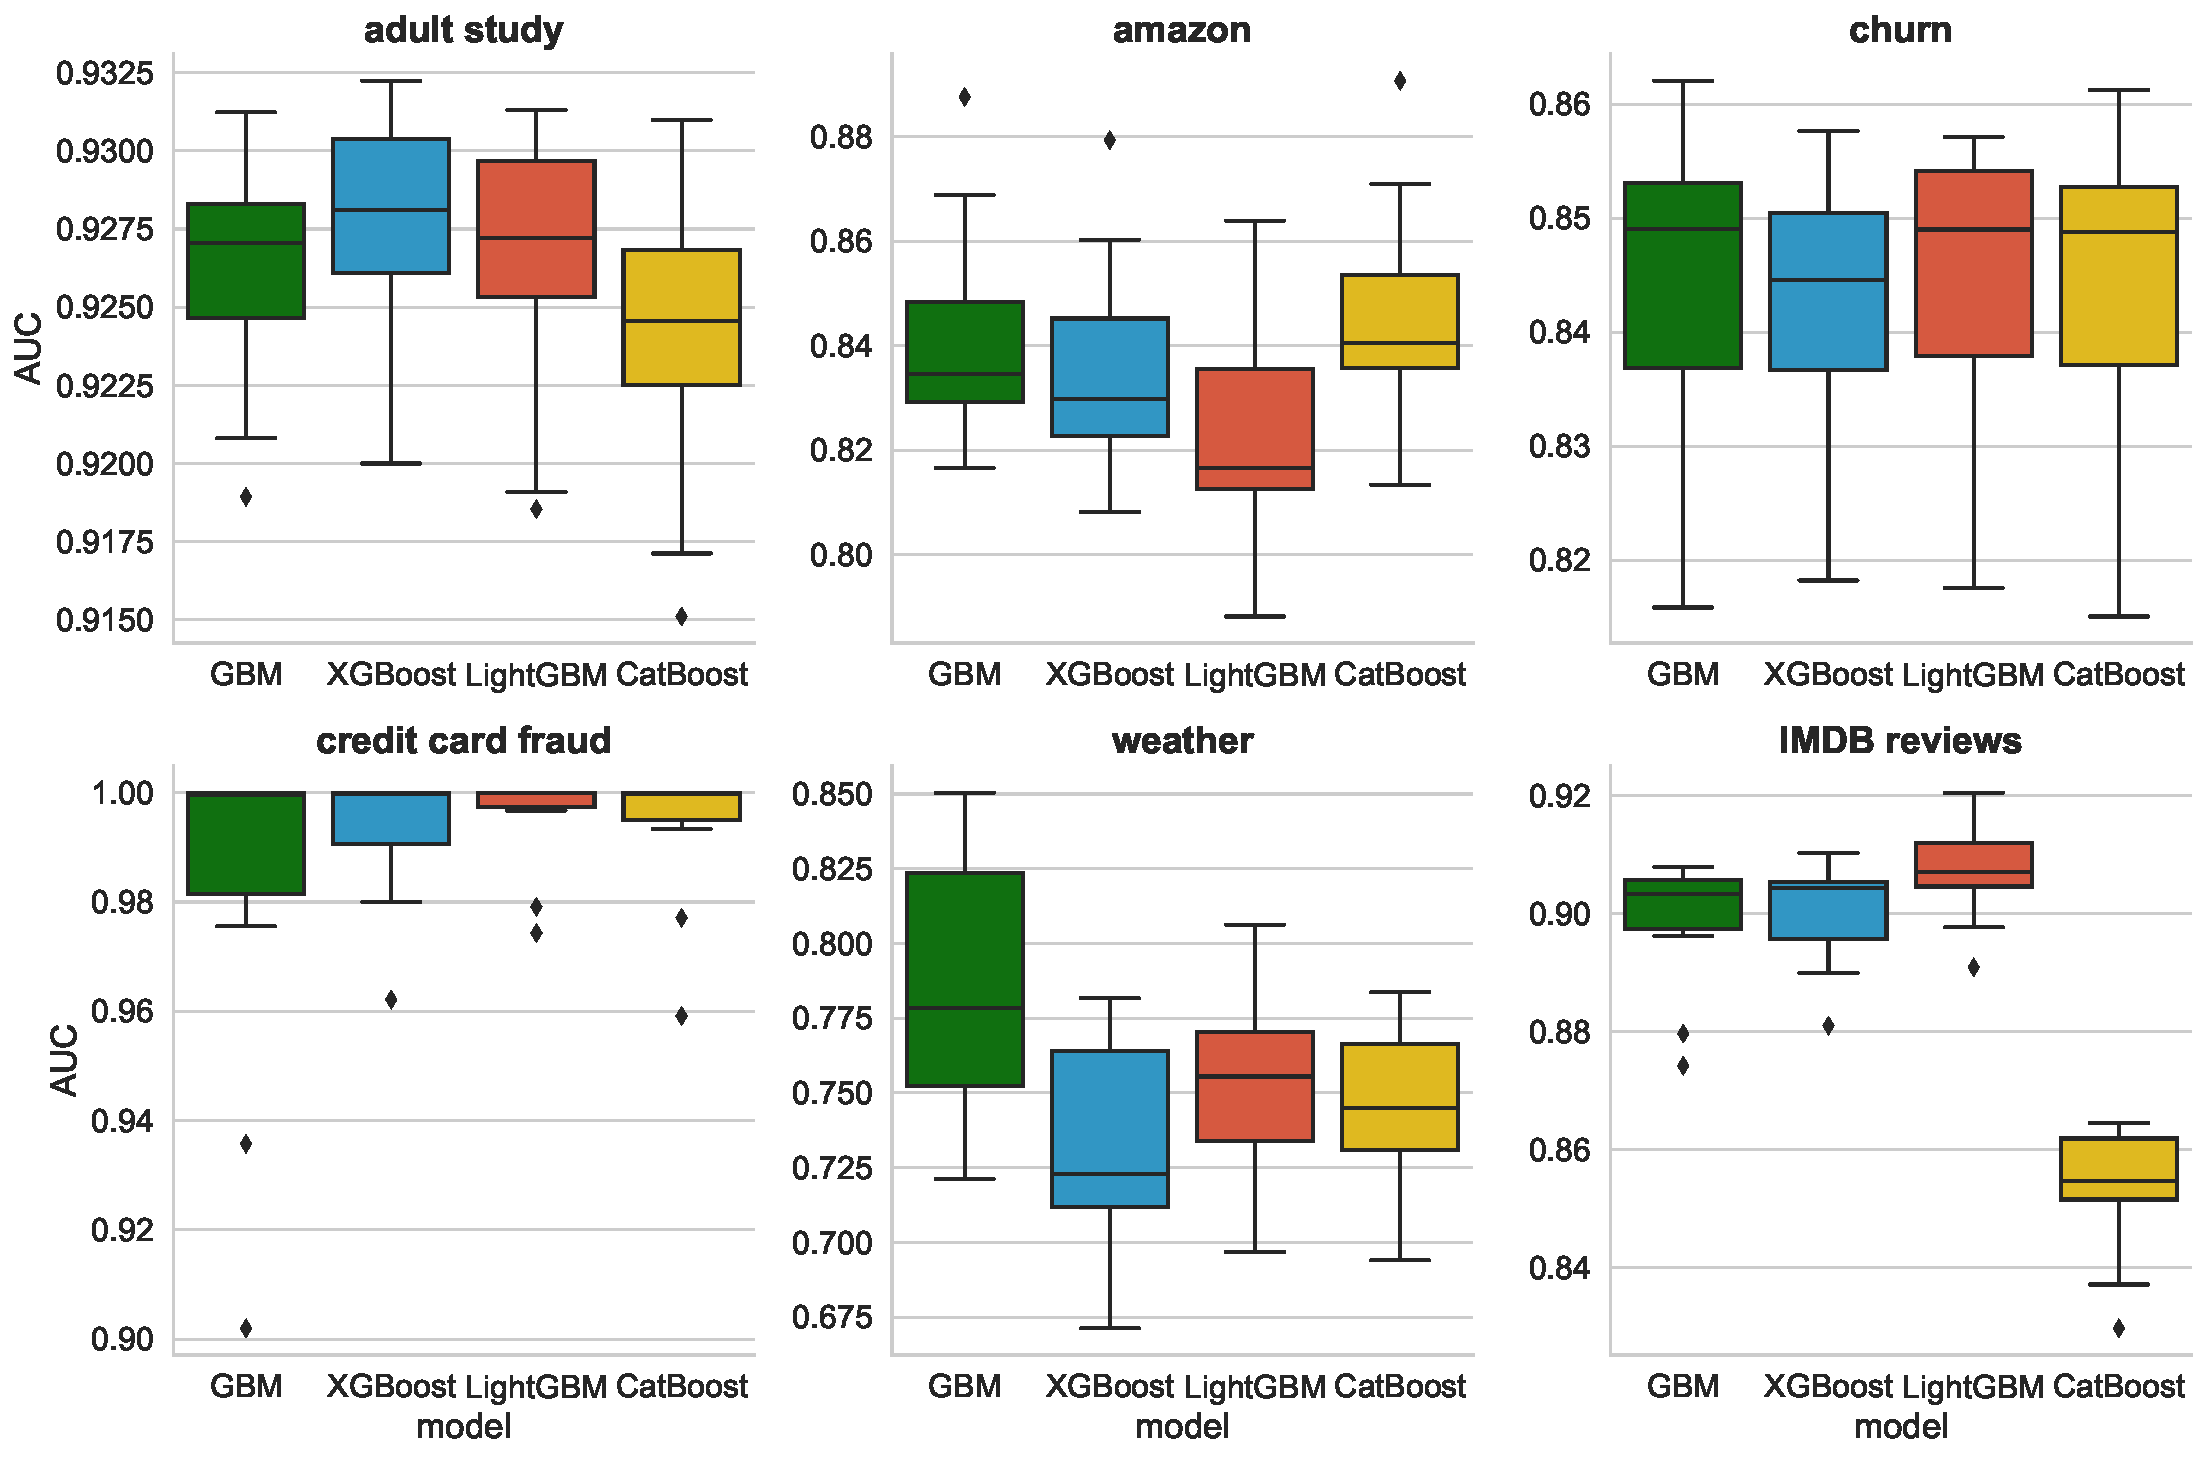
\includegraphics{main/plots/results_AUC_12_datasets_TPE_150_50_trees_facet.pdf}}
	\caption{AUC distributions across 12 datasets with TPE tuning}
	\label{fig:tpe_AUC}
\end{figure}

In terms of accuracy, LightGBM seems to be the most consistent, in case of some datasets it performs the best and it is the worst only on the \emph{prostate} dataset (mean accuracy scores for LightGBM and XGBoost are equal, but LightGBM's accuracy has higher standard deviation). Numerical results confirm that GBM and CatBoost perform very similarly. Identical observations can be made in the case of F1 score.
Results for means and standard deviations of AUC have been presented in Table~\ref{tab:tpe_AUC}.

\begin{table}[h!]
\centering
\begin{tabular}{|c|c|c|c|c|}
\hline
\textbf{dataset}  & \textbf{GBM}  & \textbf{XGBoost}  & \textbf{LightGBM}  & \textbf{CatBoost} \\ \hline
adult study & 0.926 $\pm$ 0.004 & \cellcolor{green}0.927 $\pm$ 0.004 & 0.926 $\pm$ 0.004 & \cellcolor{red}0.924 $\pm$ 0.005\\ \hline
heart disease & \cellcolor{red}0.895 $\pm$ 0.062 & 0.899 $\pm$ 0.056 & \cellcolor{green}0.914 $\pm$ 0.055 & 0.906 $\pm$ 0.051\\ \hline
amazon & 0.842 $\pm$ 0.022 & 0.835 $\pm$ 0.022 & \cellcolor{red}0.822 $\pm$ 0.024 & \cellcolor{green}0.845 $\pm$ 0.023\\ \hline
mushrooms & 1.0 $\pm$ 0.0 & 1.0 $\pm$ 0.0 & 1.0 $\pm$ 0.0 & 1.0 $\pm$ 0.0\\ \hline
breast cancer & \cellcolor{red}0.993 $\pm$ 0.012 & 0.994 $\pm$ 0.01 & \cellcolor{green}0.995 $\pm$ 0.01 & 0.994 $\pm$ 0.011\\ \hline
churn & 0.845 $\pm$ 0.014 & \cellcolor{red}0.843 $\pm$ 0.012 & \cellcolor{green}0.845 $\pm$ 0.013 & 0.844 $\pm$ 0.014\\ \hline
credit card fraud & \cellcolor{red}0.981 $\pm$ 0.035 & 0.993 $\pm$ 0.013 & \cellcolor{green}0.995 $\pm$ 0.01 & 0.993 $\pm$ 0.014\\ \hline
prostate & \cellcolor{green}0.968 $\pm$ 0.062 & 0.968 $\pm$ 0.075 & 0.964 $\pm$ 0.076 & \cellcolor{red}0.952 $\pm$ 0.08\\ \hline
leukemia & \cellcolor{red}0.973 $\pm$ 0.064 & 0.98 $\pm$ 0.063 & 0.977 $\pm$ 0.063 & \cellcolor{green}0.99 $\pm$ 0.032\\ \hline
gina agnostic & 0.985 $\pm$ 0.005 & 0.983 $\pm$ 0.005 & \cellcolor{green}0.986 $\pm$ 0.005 & \cellcolor{red}0.971 $\pm$ 0.009\\ \hline
weather & \cellcolor{green}0.786 $\pm$ 0.043 & \cellcolor{red}0.732 $\pm$ 0.036 & 0.754 $\pm$ 0.033 & 0.745 $\pm$ 0.029\\ \hline
IMDB reviews & 0.898 $\pm$ 0.012 & 0.9 $\pm$ 0.009 & \cellcolor{green}0.908 $\pm$ 0.009 & \cellcolor{red}0.853 $\pm$ 0.012\\ \hline
\end{tabular}
\caption{Means and standard deviations of AUC distributions presented in Figure~\ref{fig:tpe_AUC}}
\label{tab:tpe_AUC}
\end{table}

LightGBM is clearly the best when considering AUC scores. The average accuracies for each dataset are often the highest and standard deviations are the lowest. Tuned versions of GBM, XGBoost, LightGBM and CatBoost tend to perform very similarly on the datasets with low to medium number of features, however, some differenced can be observed on highly dimensional datasets. CatBoost's performance there is quite worrying, on the other hand LightGBM handles sparse data (\emph{gina agnostic} and \emph{IMDB reviews} datasets) the best (most likely due to the sparsity-aware splitting algorithm alongside with Exclusive Feature Bundling).

Overall, it can be concluded that hyperparameter tuning using Bayesian optimization has leveled out the performances of each of the gradient boosting implementation. However, it is not certain whether tuned models are actually better than the baseline ones presented in Section~\ref{section:baseline}. The differences of accuracy and AUC scores between the tuned and non-tuned variants of GBM, XGBoost, LightGBM and CatBoost have been presented in Table~\ref{tab:no_tuning_tpe_accuracy_diff} and ~\ref{tab:no_tuning_tpe_AUC_diff}, respectively.

   \begin{sidewaystable}
     \centering
     \begin{tabular}{c|cccccccc}
\hline
\textbf{dataset} &
\textbf{\begin{tabular}[c]{@{}c@{}}GBM\\ mean\end{tabular}} &
\textbf{\begin{tabular}[c]{@{}c@{}}GBM\\ sdev\end{tabular}} &
\textbf{\begin{tabular}[c]{@{}c@{}}XGBoost\\ mean\end{tabular}} &
\textbf{\begin{tabular}[c]{@{}c@{}}XGBoost\\ sdev\end{tabular}} &
\textbf{\begin{tabular}[c]{@{}c@{}}LightGBM\\ mean\end{tabular}} &
\textbf{\begin{tabular}[c]{@{}c@{}}LightGBM\\ sdev\end{tabular}} &
\textbf{\begin{tabular}[c]{@{}c@{}}CatBoost\\ mean\end{tabular}} &
\textbf{\begin{tabular}[c]{@{}c@{}}CatBoost\\ sdev\end{tabular}} \\ \hline
adult study & +0.225\% & -10.035\% & +0.36\% & +38.802\% & +0.209\% & +18.611\% & -0.465\% & +18.35\%\\ \hline
heart disease & +2.893\% & -14.776\% & +2.395\% & -7.015\% & +0.805\% & +0.007\% & -0.383\% & -0.975\%\\ \hline
amazon & +0.068\% & +45.611\% & -0.2\% & +10.491\% & +0.084\% & +45.447\% & -0.052\% & +87.512\%\\ \hline
mushrooms & 0.0\% & 0.0\% & 0.0\% & 0.0\% & 0.0\% & 0.0\% & +0.012\% & -100.0\%\\ \hline
breast cancer & 0.0\% & +6.5\% & -0.901\% & -1.527\% & +0.363\% & -15.385\% & +0.181\% & +9.296\%\\ \hline
churn & +0.532\% & +32.333\% & +2.204\% & -24.691\% & +3.213\% & -46.033\% & +0.515\% & -23.365\%\\ \hline
credit card fraud & +0.037\% & -34.581\% & -0.003\% & +1.411\% & +0.291\% & -88.242\% & +0.01\% & +0.927\%\\ \hline
prostate & +3.261\% & -10.358\% & 0.0\% & 0.0\% & +6.818\% & -25.722\% & 0.0\% & 0.0\%\\ \hline
leukemia & +8.439\% & -22.171\% & -1.509\% & +1.802\% & +3.162\% & +3.705\% & 0.0\% & 0.0\%\\ \hline
gina agnostic & +2.39\% & -38.174\% & -1.276\% & +6.957\% & -0.579\% & +45.392\% & -3.277\% & +51.498\%\\ \hline
weather & +6.331\% & +54.748\% & -8.215\% & +4.31\% & +1.234\% & -29.377\% & -0.897\% & +15.341\%\\ \hline
IMDB reviews & +6.169\% & +43.014\% & -0.694\% & +21.516\% & +0.279\% & +11.814\% & -8.401\% & +38.744\%\\ \hline
\end{tabular}
\caption{Percentage gain/loss of values of means and standard deviations of accuracy --- TPE tuning vs no tuning}
\label{tab:no_tuning_tpe_accuracy_diff}

    \vspace{1.5\baselineskip}
     \centering
     \begin{tabular}{c|cccccccc}
\hline
\textbf{dataset} &
\textbf{\begin{tabular}[c]{@{}c@{}}GBM\\ mean\end{tabular}} &
\textbf{\begin{tabular}[c]{@{}c@{}}GBM\\ sdev\end{tabular}} &
\textbf{\begin{tabular}[c]{@{}c@{}}XGBoost\\ mean\end{tabular}} &
\textbf{\begin{tabular}[c]{@{}c@{}}XGBoost\\ sdev\end{tabular}} &
\textbf{\begin{tabular}[c]{@{}c@{}}LightGBM\\ mean\end{tabular}} &
\textbf{\begin{tabular}[c]{@{}c@{}}LightGBM\\ sdev\end{tabular}} &
\textbf{\begin{tabular}[c]{@{}c@{}}CatBoost\\ mean\end{tabular}} &
\textbf{\begin{tabular}[c]{@{}c@{}}CatBoost\\ sdev\end{tabular}} \\ \hline
adult study & +0.281\% & -15.696\% & +0.141\% & +3.778\% & +0.281\% & -2.272\% & -0.518\% & +23.227\%\\ \hline
heart disease & +2.207\% & -3.913\% & +2.39\% & +0.236\% & +1.201\% & +4.594\% & +0.75\% & -7.96\%\\ \hline
amazon & +2.837\% & +13.254\% & +1.226\% & +16.862\% & -0.704\% & +14.502\% & +1.609\% & +7.323\%\\ \hline
mushrooms & 0.0\% & +216.228\% & 0.0\% & -100.0\% & 0.0\% & 0.0\% & 0.0\% & -100.0\%\\ \hline
breast cancer & -0.112\% & +9.288\% & -0.027\% & +2.344\% & +0.159\% & -31.696\% & +0.053\% & -9.179\%\\ \hline
churn & +0.688\% & +18.875\% & +3.18\% & -4.343\% & +3.805\% & -8.839\% & +0.565\% & -3.227\%\\ \hline
credit card fraud & +5.143\% & -51.348\% & +0.466\% & -37.012\% & +23.897\% & -95.758\% & +0.48\% & -31.941\%\\ \hline
prostate & +2.542\% & -25.0\% & +0.415\% & +17.47\% & 0.0\% & +73.734\% & -0.833\% & +2.326\%\\ \hline
leukemia & +2.277\% & -17.382\% & 0.0\% & 0.0\% & +0.861\% & -3.154\% & -1.0\% & 0\%\\ \hline
gina agnostic & +1.333\% & -22.642\% & -0.405\% & +11.921\% & +0.014\% & +15.313\% & -1.296\% & +68.488\%\\ \hline
weather & +4.62\% & +35.32\% & -5.549\% & -23.271\% & +0.138\% & -20.273\% & -0.432\% & -23.948\%\\ \hline
IMDB reviews & +4.211\% & +9.168\% & -0.315\% & -0.261\% & +0.084\% & -7.264\% & -5.938\% & +15.504\%\\ \hline
\end{tabular}
\caption{Percentage gain/loss of values of means and standard deviations of AUC --- TPE tuning vs no tuning}
\label{tab:no_tuning_tpe_AUC_diff}
   \end{sidewaystable}

When looking at the change of mean values of accuracy and AUC one can notice that TPE tuning has increased the performance of GBM, XGBoost, LightGBM and CatBoost in terms of the mean values. The absolute value of the means in case of accuracy and AUC usually does not exceed 10\%. The most negative change of mean has been observed in the case of CatBoost's accuracy on the \emph{IMDB reviews} dataset --- TPE tuning has decreased the performance of the model by around 8.4\%. On the other hand, the biggest gain has been recorded in case of LightGBM. Mean AUC on the \emph{credit card fraud} dataset has increased by almost 24\%. On the other hand, standard deviations changed much more drastically, either positively or negatively. After TPE tuning, the standard deviations have to be considered on case-by-case basis, one model and one dataset at a time. Similar conclusions can be drawn by considering F1 score instead of accuracy or AUC.

Bayesian optimization in itself is quite slow due to its sequential nature --- tuning times of the algorithms have been presented in Figure~\ref{fig:tpe_tuning_times}.

\begin{figure}[H]
	\centering
		\scalebox{0.42}{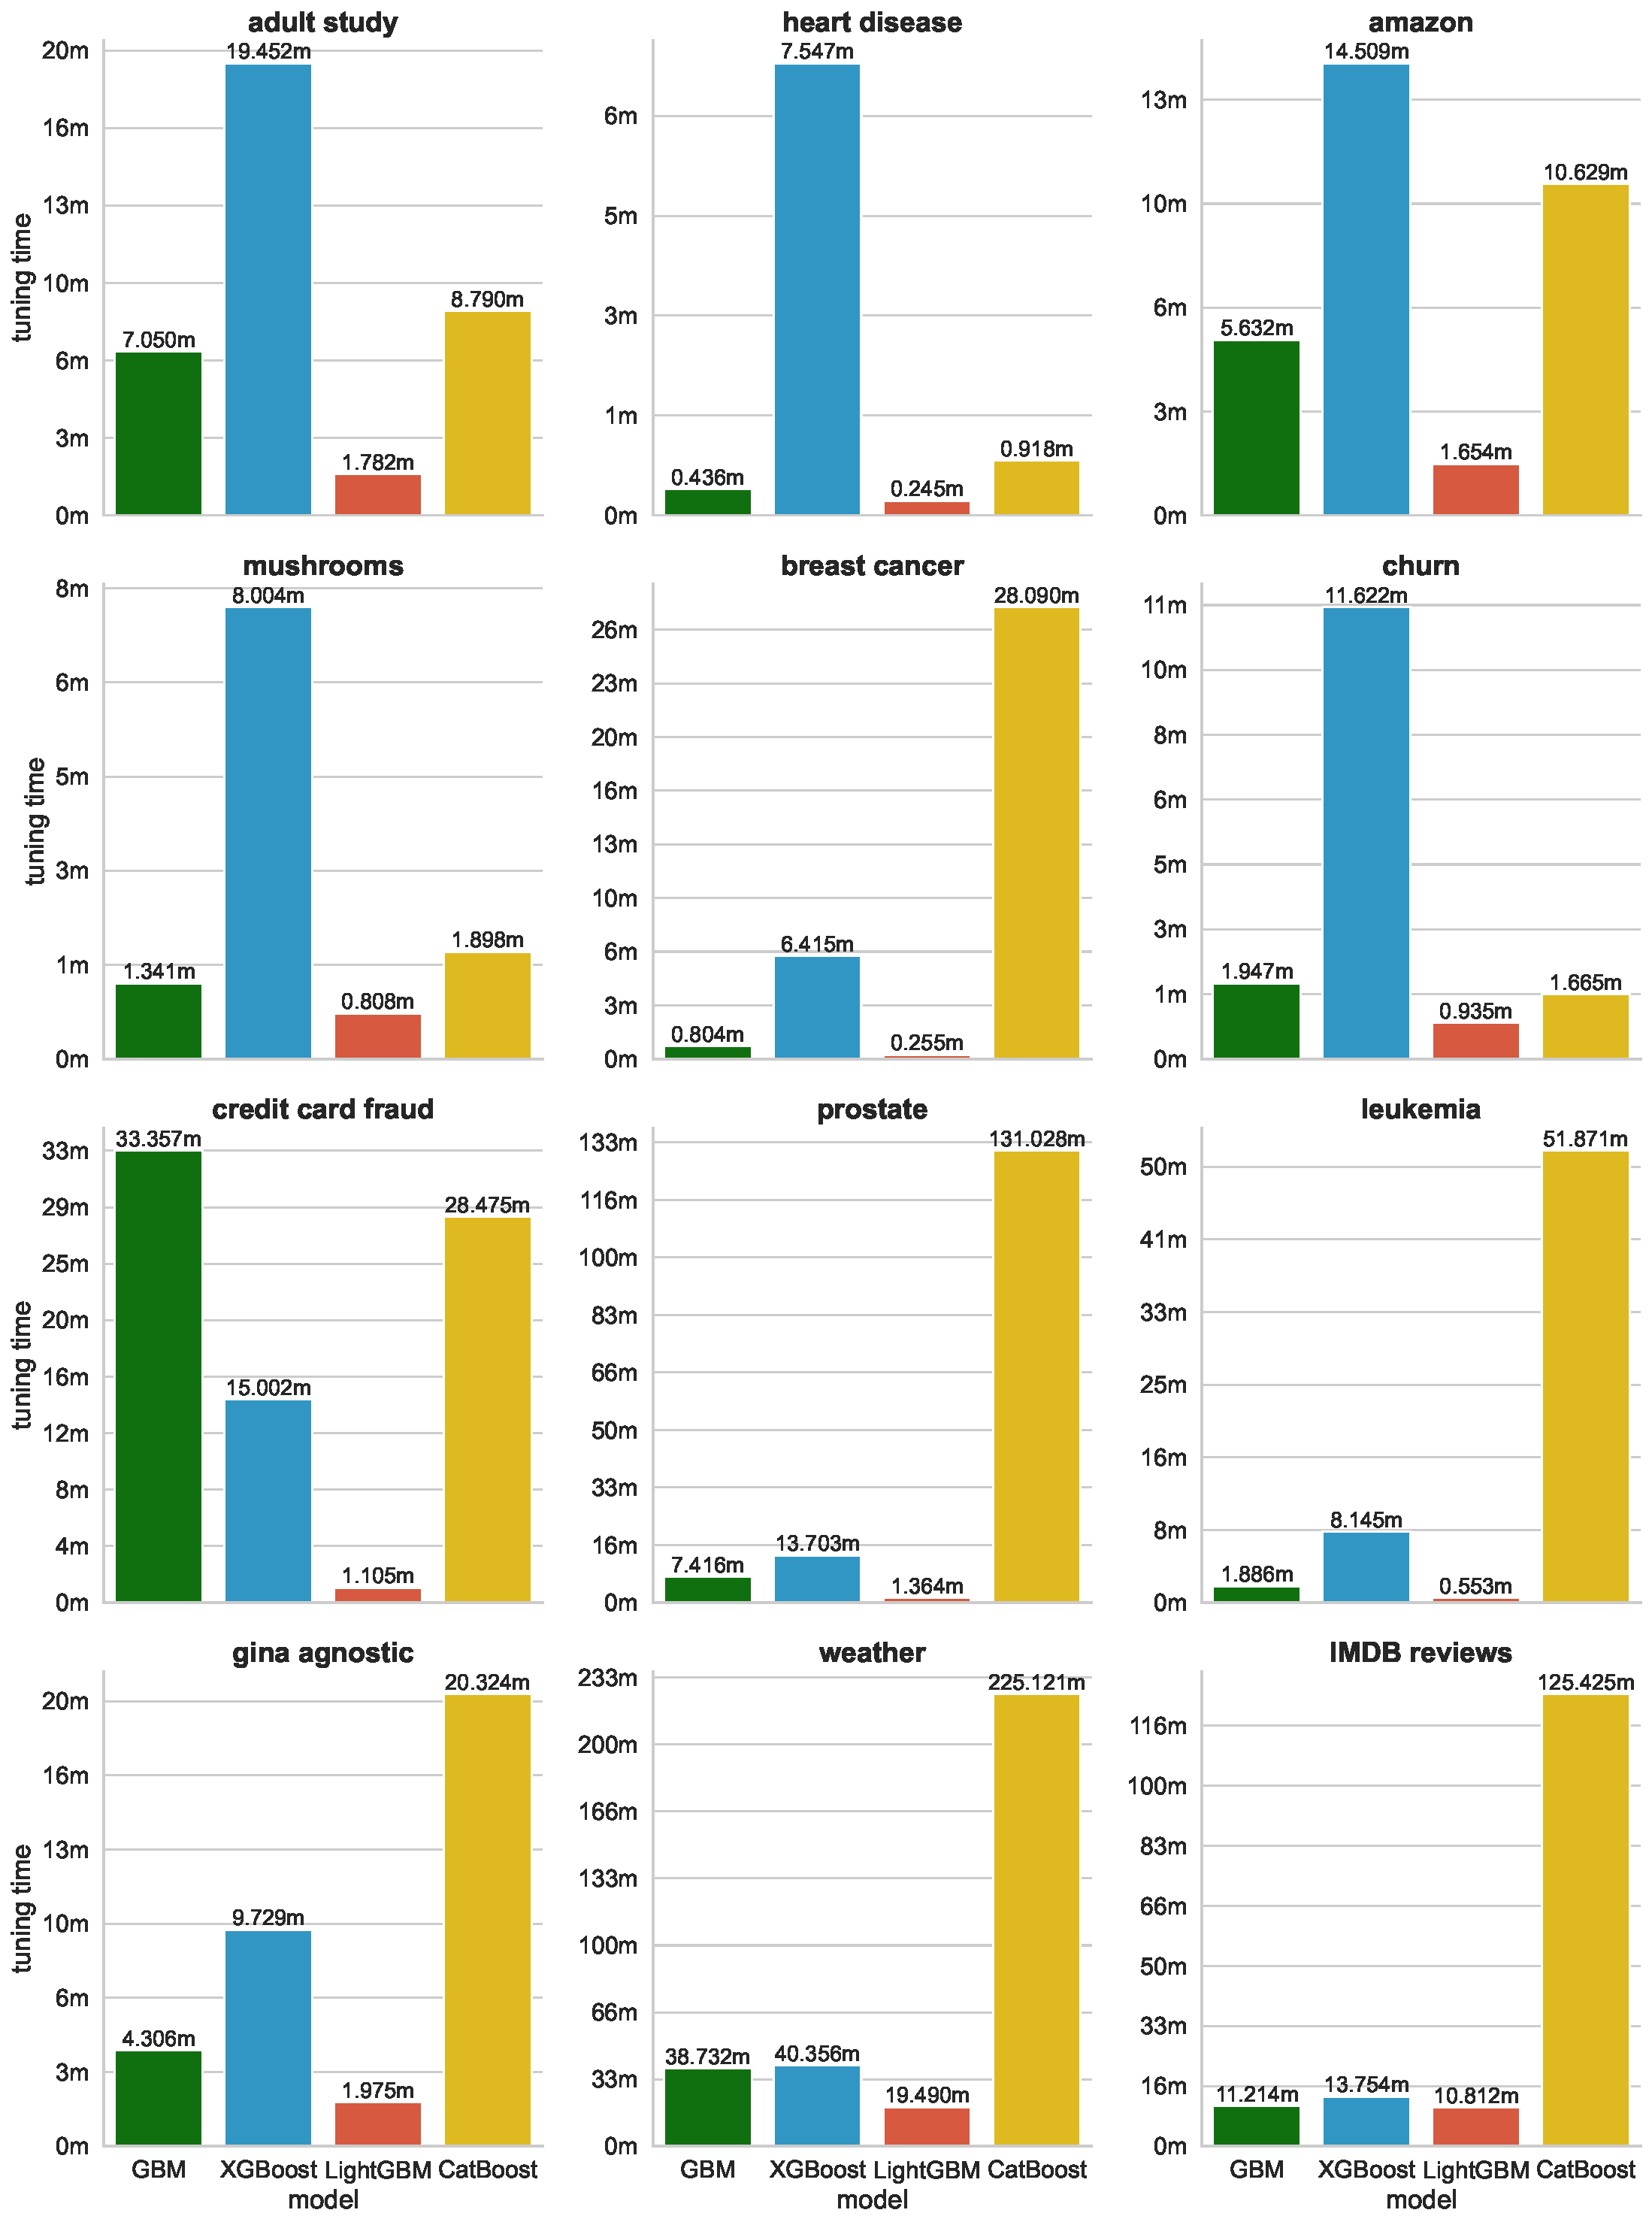
\includegraphics{main/plots/tuning_times_12_datasets_TPE_150_50_trees_facet.pdf}}
	\caption{Tuning times of the models across 12 datasets with TPE tuning}
	\label{fig:tpe_tuning_times}
\end{figure}

Additional time to perform model selection is quite long --- in the case of datasets with a reasonable number of features it can be stated that the time consumed to perform hyperparameter tuning is worth the slight increase of models' performance in terms of accuracy, F1 score and AUC. The situation is different on highly dimensional datasets, especially in case of CatBoost which is very inefficient (also, surprisingly it is highly inefficient for \emph{breast cancer} dataset). Two or three hour long hyperparameter tuning in case of CatBoost is not worth the time spent, especially that in the case of the \emph{IMDB reviews} dataset the tuning was actually counterproductive. On the other hand, GBM seems to be quite fast, XGBoost is slightly less consistent. The algorithm which benefited the most from the tuning is also the most efficient --- LightGBM is lightning fast. The difference of the tuning times compared to other models is enormous --- the tuning times are often lower by one or two orders of magnitude. The difference is the biggest in the case of the \emph{breast cancer} dataset; LightGBM is over 100 times faster (in other words, one could perform TPE tuning over the span of 1500 iterations instead of 15 and there is a high chance that LightGBM would still complete the tuning process faster than CatBoost). It can be stated that LightGBM is the GBM implementation of choice for performing hyperparameter tuning due to a significant increase in performance as well as enormous scalability and efficiency.

The runtimes of the models selected in the hyperparameter tuning have been presented in Figure~\ref{fig:tpe_runtimes}.

\begin{figure}[H]
	\centering
		\scalebox{0.42}{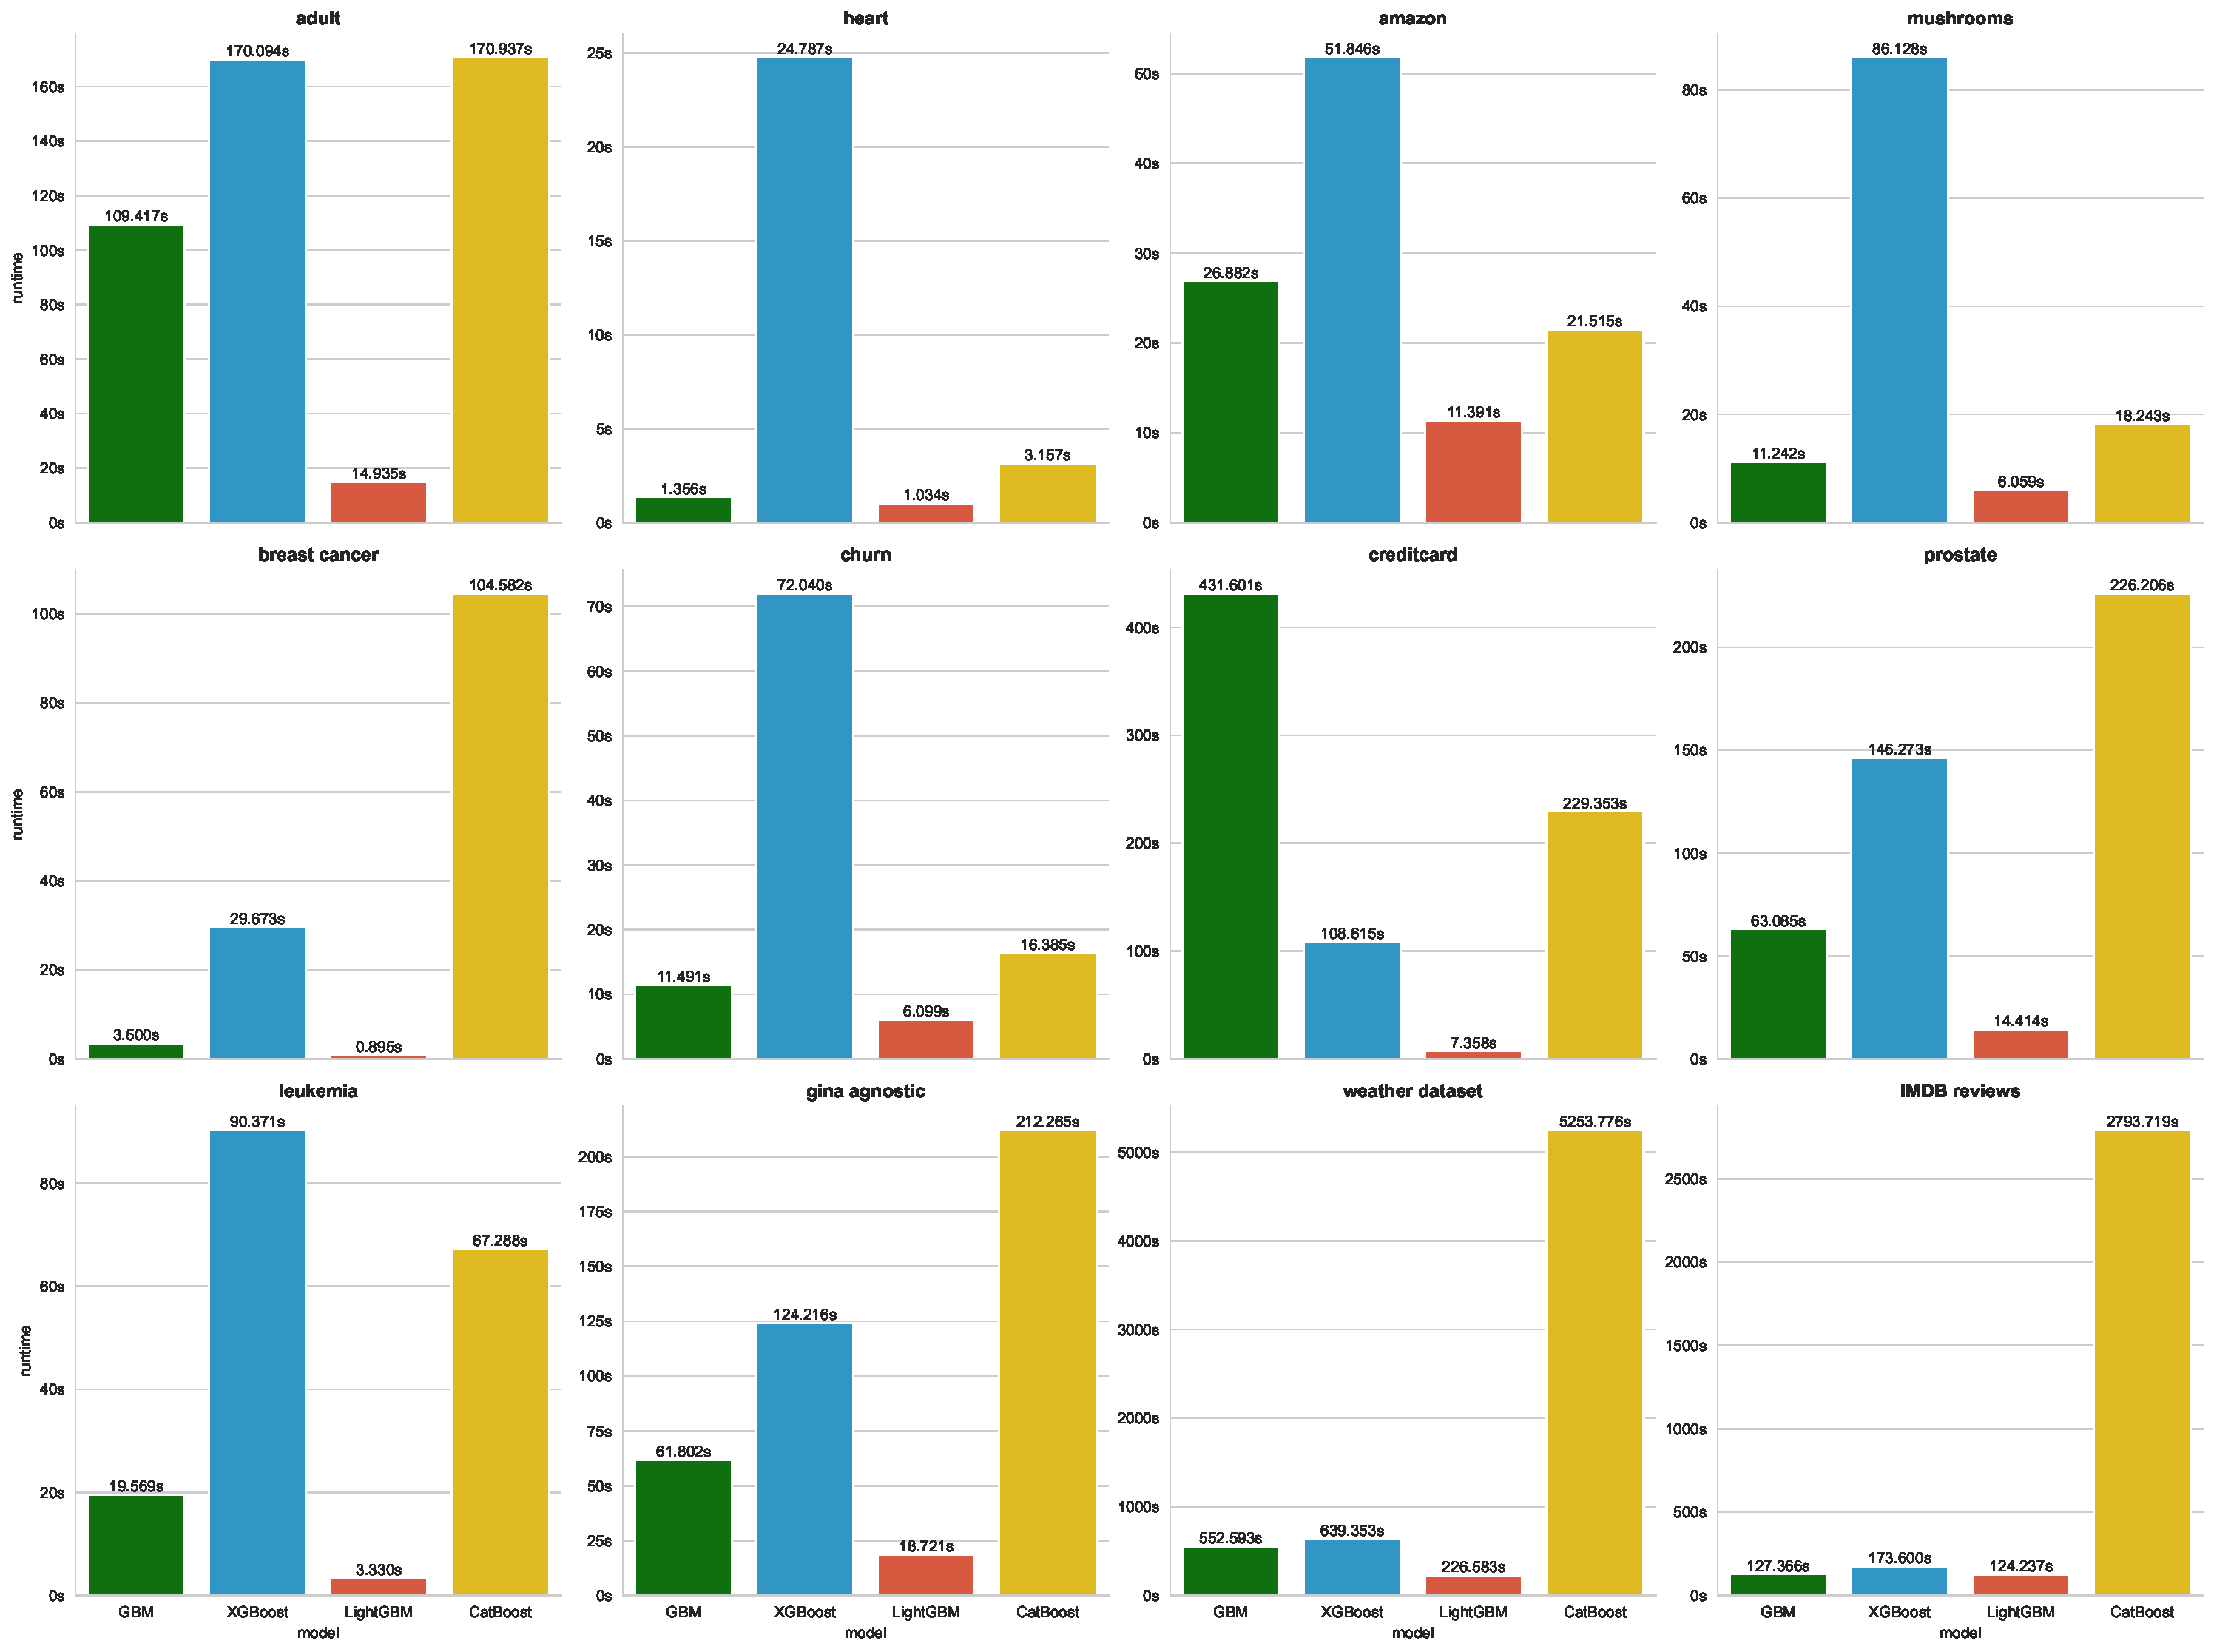
\includegraphics{main/plots/runtimes_12_datasets_TPE_150_50_trees_facet.pdf}}
	\caption{Runtimes of the models across 12 datasets with TPE tuning}
	\label{fig:tpe_runtimes}
\end{figure}

In general, the runtimes of the tuned models are lower than those of baseline ones. Regularization has definitely helped to decrease the runtime, as well as randomization in form of instance and feature subsampling. On the other hand, higher runtimes may be due to the fact that the \emph{max\_depth} hyperparameter was tuned. In some cases, the best model chosen by TPE tuning could grow trees up to 10 levels deep, which would greatly increase the runtime (by default, GBM models use shallower trees with 4-6 levels).

In order to rank GBM, XGBoost, LightGBM and CatBoost tuned using Tree Parzen Estimators, Friedman test with Nemenyi post hoc analysis has been performed. Ranking in case of F1 score has been presented in Figure~\ref{fig:tpe_F1_heatmap}.

\begin{figure}[H]
	\centering
		\scalebox{0.7}{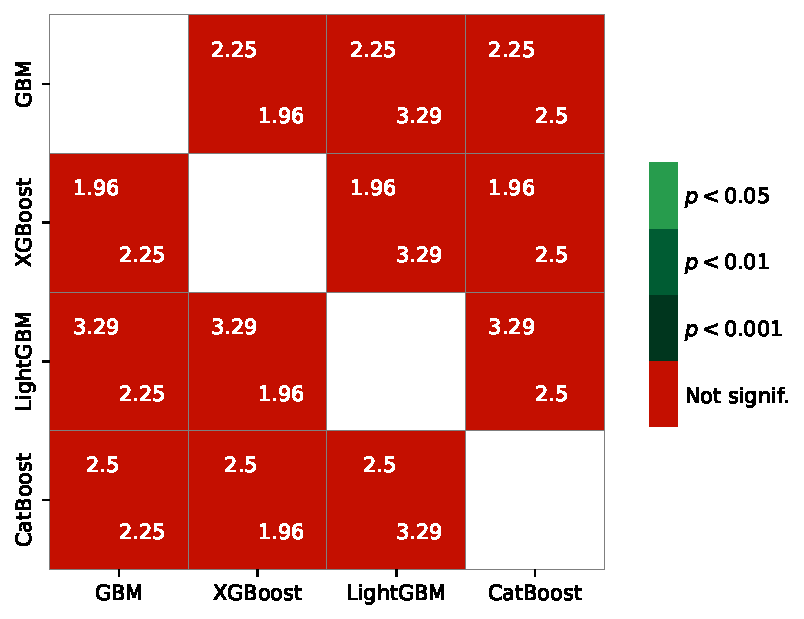
\includegraphics{main/plots/heatmap_f1_score_12_datasets_TPE_150_50_trees.pdf}}
	\caption{Ranking of tuned models' F1 scores. Critical difference $CD = 1.354$}
	\label{fig:tpe_F1_heatmap}
\end{figure}

Every difference in the rankings is lower than the critical difference threshold equal to 1.354. The ranks for GBM, XGBoost and CatBoost are quite close, but LightGBM is ranked much higher. The difference between the worst and the best model --- XGBoost and LightGBM equal to 1.33 which is very close to the critical difference is not statistically significant, but it is apparent that tuned LightGBM is in fact better than tuned XGBoost (the difference in performance can be observed in Figures~\ref{fig:tpe_accuracy}, \ref{fig:tpe_AUC} and Tables~\ref{tab:tpe_accuracy} and \ref{tab:tpe_AUC}). In case of accuracy and AUC metrics, the rankings are similar to the one presented in Figure~\ref{fig:tpe_F1_heatmap}, although all pairwise comparison of models indicate that differences in performance are still statistically significant.

Finally, it was essential to use the Friedman test with Nemenyi post hoc analysis to determine the rankings of 8 models: the baseline versions of GBM, XGBoost, LightGBM and CatBoost and their tuned counterparts. From the visual analysis it can be inferred that tuned LightGBM is the best model, overall and baseline gradient boosting is the worst one. The ranking of algorithms excluding the two aforementioned models is not clear --- that is why the Friedman test will help to prepare such ranking in the most objective way. The heatmap with the rankings of performance in terms of AUC of all eight models have been presented in Figure~\ref{fig:no_tuning_tpe_AUC_heatmap}.

\begin{figure}[H]
	\centering
		\scalebox{0.8}{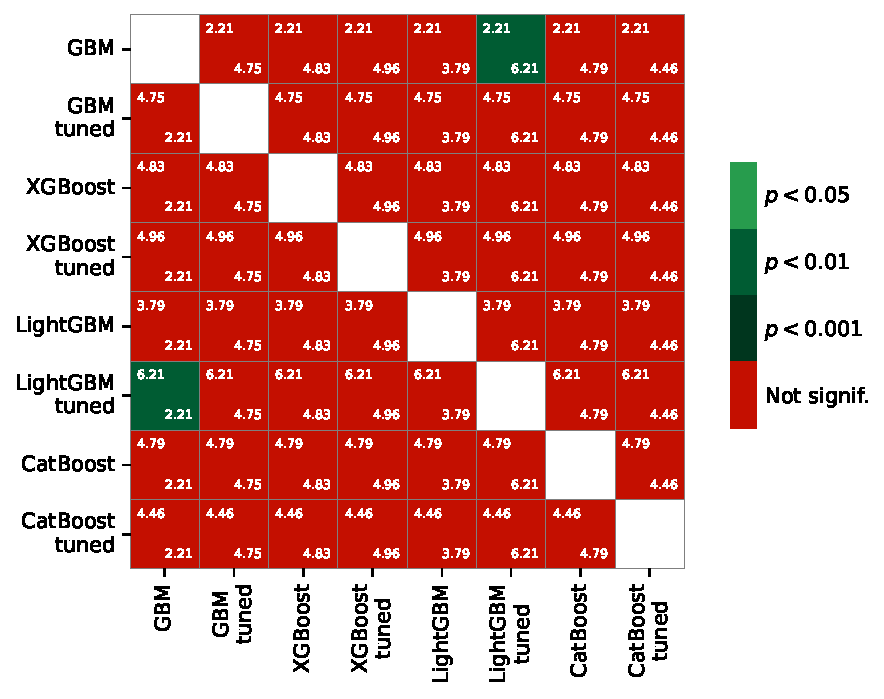
\includegraphics{main/plots/heatmap_AUC_combined_TPE_150_50_trees.pdf}}
	\caption{Ranking of tuned models' F1 scores. Critical difference $CD = 3.031$}
	\label{fig:no_tuning_tpe_AUC_heatmap}
\end{figure}

Friedman test with Nemenyi post hoc analysis implies that there is only one case where the pairwise comparison of rankings of two models is statistically significant --- the performance of tuned LightGBM is statistically different (in this case better) than the performance of baseline GBM. A similar pattern can be observed in the case of rankings obtained for accuracy and F1 score, but in those cases the p-value of the Nemenyi test was higher ($p<0.05$ compared to $p<0.01$ in case of AUC). In case of all three aforementioned evaluation metrics, the rankings are quite similar --- tuned LightGBM is the best by a big margin in the rank, then models such as XGBoost, tuned XGBoost, CatBoost and tuned CatBoost and tuned GBM can be considered as the next best models (although not always in that particular order), however, the difference in their ranks is quite small. Lastly, two worst algorithms are LightGBM and GBM which is not surprising.

\subsection{Comparison between randomized search, Bayesian optimization and no tuning}\label{section_rand}
In Sections~\ref{section:baseline} and \ref{section_tpe} comparative analysis of baseline and tuned variants of GBM, XGBoost, LightGBM and CatBoost has been conducted. The method of choice for hyperparameter tuning was Bayesian optimization using Tree Parzen Estimators. In this section, a different method used for model selection will be analyzed, namely the randomized search. Bayesian optimization has proven to be effective, but quite time consuming and computationally demanding, thus it is reasonable to check if simpler methods, such as aforementioned randomized search can be a better alternative.

Each iteration of randomized search is independent from each other, so the tuning procedure can be parallelized --- thus, it is expected that 15 iterations of randomized search will take less time than tuning using Tree Parzen Estimators. Therefore, the number of iterations has been set to 30 --- the differences of tuning times between two aforementioned model selection methods have been presented in Figure~\ref{fig:diffs}.

\begin{figure}[H]
	\centering
		\scalebox{0.42}{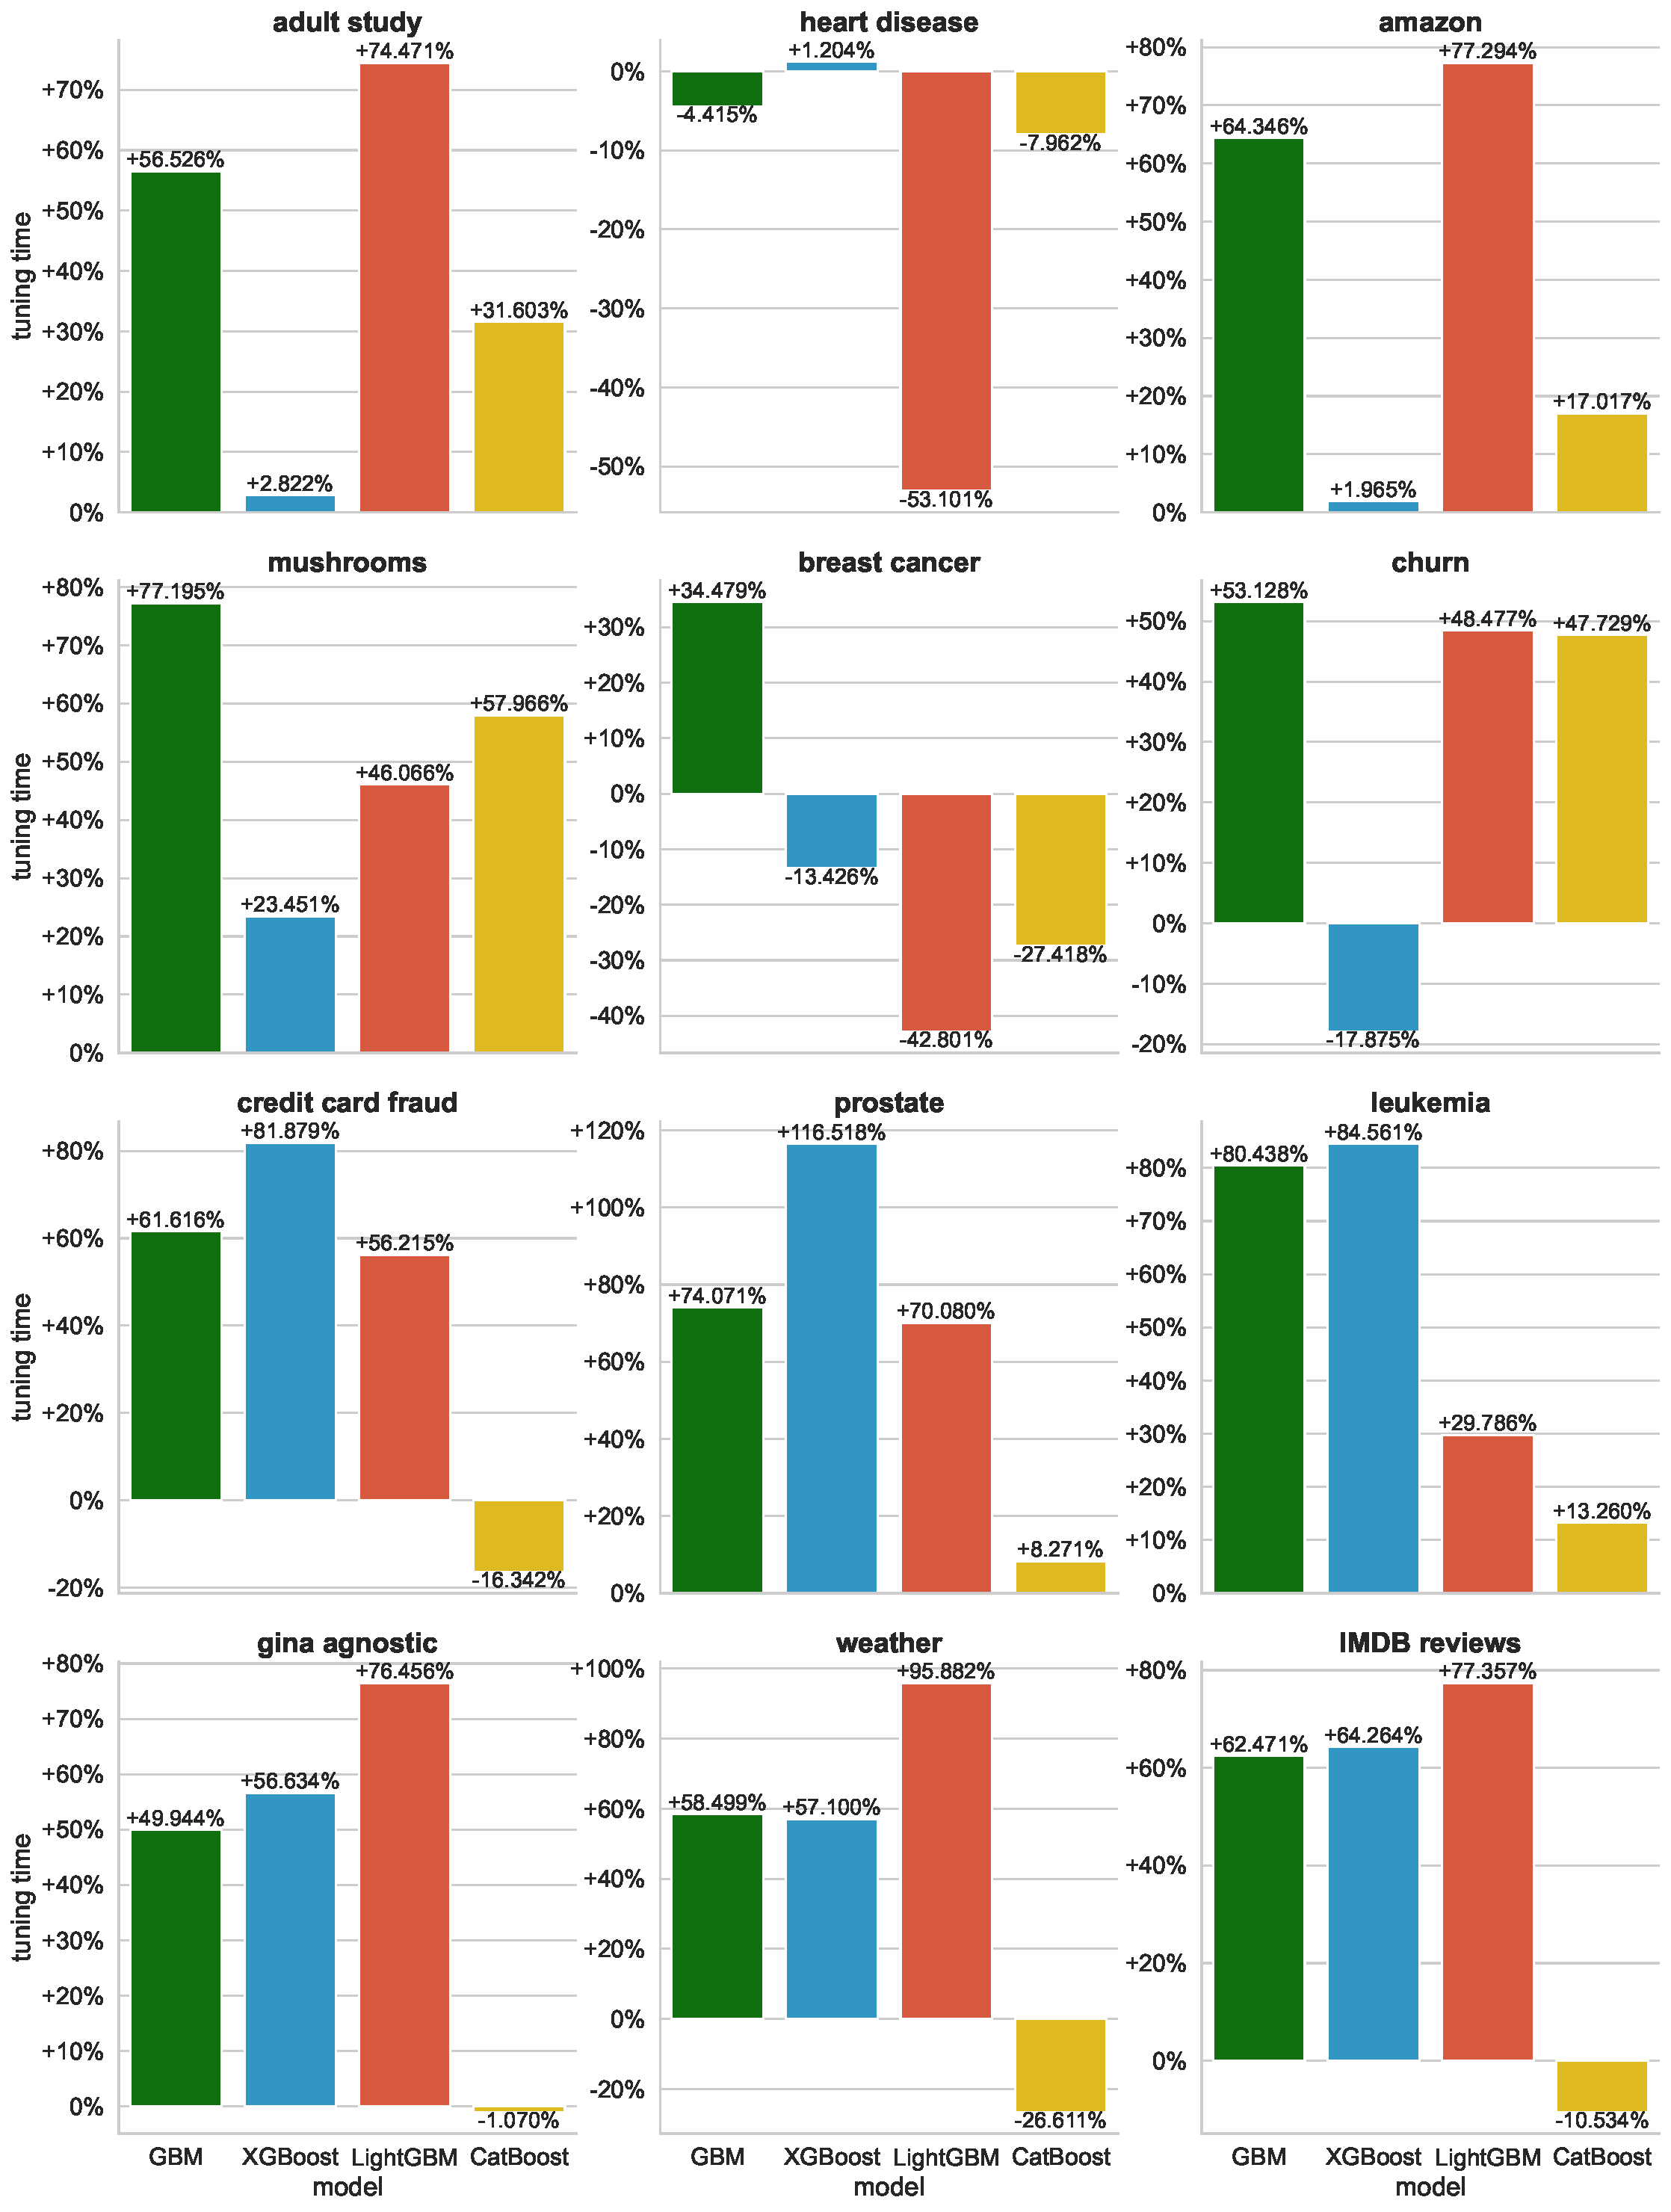
\includegraphics{main/plots/diffs_barplots.pdf}}
	\caption{Differences between tuning times using randomized search and Bayesian optimization}
	\label{fig:diffs}
\end{figure}

On most of the datasets, randomized search took longer time than TPE tuning. In some cases the time to complete model selection was longer by over 50\%, but sometimes randomized search was faster.

It is essential to compare the performance of both types of hyperparameter tuning and the case where there was no tuning performed. The comparison has been performed for each GBM implementation: GBM, XGBoost, LightGBM and CatBoost and each evaluation metric: accuracy, F1 score and AUC in the following scenarios:

\begin{enumerate}
    \item no tuning vs Bayesian optimization using TPE,
    \item no tuning vs randomized search,
    \item Bayesian optimization vs randomized search.
\end{enumerate}

All pairwise tests have been performed using the Wilcoxon signed-ranks Test with one-sided alternative hypothesis. The results have been compiled in Table~\ref{tab:no_tuning_tpe_rand}.

\begin{table}[h!]
\centering
\begin{tabular}{|c|c|c|c|c|}
\hline
\textbf{model} & \diagbox{\textbf{metric}}{\textbf{case}}         & \textbf{no tuning | TPE} & \textbf{no tuning | rand.} & \textbf{TPE | rand.} \\ \hline
               & accuracy & TPE                       & randomized                 & $p > 0.05$                 \\ \cline{2-5}
GBM            & F1 score & TPE                       & randomized                 & $p > 0.05$                 \\ \cline{2-5}
               & AUC      & TPE                       & randomized                 & $p > 0.05$                 \\ \hline
               & accuracy & $p > 0.05$                      & $p > 0.05$                       & $p > 0.05$                 \\ \cline{2-5}
XGBoost        & F1 score & $p > 0.05$                      & $p > 0.05$                       & randomized           \\ \cline{2-5}
               & AUC      & $p > 0.05$                      & $p > 0.05$                       & $p > 0.05$                 \\ \hline
               & accuracy & TPE                       & randomized                 & randomized           \\ \cline{2-5}
LightGBM       & F1 score & TPE                       & randomized                 & randomized           \\ \cline{2-5}
               & AUC      & TPE                       & randomized                 & randomized           \\ \hline
               & accuracy & $p > 0.05$                      & $p > 0.05$                       & $p > 0.05$                 \\ \cline{2-5}
CatBoost       & F1 score & $p > 0.05$                      & $p > 0.05$                       & $p > 0.05$                 \\ \cline{2-5}
               & AUC      & $p > 0.05$                      & $p > 0.05$                       & $p > 0.05$                 \\ \hline
\end{tabular}
\caption{Comparison of TPE and randomized search tuning in contrast to no tuning}
\label{tab:no_tuning_tpe_rand}
\end{table}

In case of GBM and LightGBM it is always more efficient to perform either TPE tuning or randomized search rather than not. On the other hand, in case of XGBoost and CatBoost no significant differences of performing hyperparameter tuning have been found --- it may imply that XGBoost and CatBoost do not have to be tuned at all.

The comparison between Bayesian optimization (15 iterations) and randomized search (30 iterations) is interesting --- the latter has proven to be better than the former when evaluating XGBoost using the F1 score. LightGBM tends to benefit from the randomized search; the usual longer tuning time compared to Bayesian optimization is worth it. It may be beneficial to pair TPE tuning with GBM, XGBoost or CatBoost.

Moreover, randomized search with 15 iterations has been tested. Overall, it is much faster than Bayesian optimization, but has not proven to be better while using LightGBM.

The final rankings of the models in terms of choice of hyperparameter tuning method and evaluation metric has been presented in Figure~\ref{tab:all_tunings_rankings}.

\newpage
\begin{table}[h!]
\centering
\begin{tabular}{|c|c|c|c|}
\hline
\textbf{\begin{tabular}[c]{@{}c@{}}model\\ rank\end{tabular}} &
  \textbf{accuracy} &
  \textbf{F1 score} &
  \textbf{AUC} \\ \hline
\textbf{\#1} &
  \begin{tabular}[c]{@{}c@{}}LightGBM\\ randomized\\ 9.75\end{tabular} &
  \begin{tabular}[c]{@{}c@{}}LightGBM\\ randomized\\ 9.62\end{tabular} &
  \begin{tabular}[c]{@{}c@{}}LightGBM\\ randomized\\ 9.46\end{tabular} \\ \hline
\textbf{\#2} &
  \begin{tabular}[c]{@{}c@{}}LightGBM\\ TPE\\ 7.54\end{tabular} &
  \begin{tabular}[c]{@{}c@{}}LightGBM\\ TPE\\ 8.25\end{tabular} &
  \begin{tabular}[c]{@{}c@{}}LightGBM\\ TPE\\ 8.38\end{tabular} \\ \hline
\textbf{\#3} &
  \begin{tabular}[c]{@{}c@{}}XGBoost\\ no tuning\\ 7.50\end{tabular} &
  \begin{tabular}[c]{@{}c@{}}CatBoost\\ no tuning\\ 7.54\end{tabular} &
  \begin{tabular}[c]{@{}c@{}}XGBoost\\ randomized\\ 7.21\end{tabular} \\ \hline
\textbf{\#4} &
  \begin{tabular}[c]{@{}c@{}}CatBoost\\ no tuning\\ 7.12\end{tabular} &
  \begin{tabular}[c]{@{}c@{}}XGBoost\\ no tuning\\ 7.50\end{tabular} &
  \begin{tabular}[c]{@{}c@{}}XGBoost\\ TPE\\ 6.88\end{tabular} \\ \hline
\textbf{\#5} &
  \begin{tabular}[c]{@{}c@{}}XGBoost\\ randomized\\ 6.88\end{tabular} &
  \begin{tabular}[c]{@{}c@{}}XGBoost\\ randomized\\ 7.04\end{tabular} &
  \begin{tabular}[c]{@{}c@{}}CatBoost\\ no tuning\\ 6.75\end{tabular} \\ \hline
\textbf{\#6} &
  \begin{tabular}[c]{@{}c@{}}GBM\\ randomized\\ 6.58\end{tabular} &
  \begin{tabular}[c]{@{}c@{}}GBM\\ randomized\\ 6.62\end{tabular} &
  \begin{tabular}[c]{@{}c@{}}XGBoost\\ no tuning\\ 6.54\end{tabular} \\ \hline
\textbf{\#7} &
  \begin{tabular}[c]{@{}c@{}}GBM\\ TPE\\ 6.50\end{tabular} &
  \begin{tabular}[c]{@{}c@{}}GBM\\ TPE\\ 6.17\end{tabular} &
  \begin{tabular}[c]{@{}c@{}}GBM\\ TPE\\ 6.50\end{tabular} \\ \hline
\textbf{\#8} &
  \begin{tabular}[c]{@{}c@{}}CatBoost\\ TPE\\ 6.17\end{tabular} &
  \begin{tabular}[c]{@{}c@{}}CatBoost\\ TPE\\ 6.08\end{tabular} &
  \begin{tabular}[c]{@{}c@{}}CatBoost\\ TPE\\ 6.21\end{tabular} \\ \hline
\textbf{\#9} &
  \begin{tabular}[c]{@{}c@{}}CatBoost\\ randomized\\ 5.71\end{tabular} &
  \begin{tabular}[c]{@{}c@{}}CatBoost\\ randomized\\ 5.50\end{tabular} &
  \begin{tabular}[c]{@{}c@{}}GBM\\ randomized\\ 6.12\end{tabular} \\ \hline
\textbf{\#10} &
  \begin{tabular}[c]{@{}c@{}}XGBoost\\ TPE\\ 5.54\end{tabular} &
  \begin{tabular}[c]{@{}c@{}}XGBoost\\ TPE\\ 5.33\end{tabular} &
  \begin{tabular}[c]{@{}c@{}}CatBoost\\ randomized\\ 5.96\end{tabular} \\ \hline
\textbf{\#11} &
  \begin{tabular}[c]{@{}c@{}}LightGBM\\ no tuning\\ 5.25\end{tabular} &
  \begin{tabular}[c]{@{}c@{}}LightGBM\\ no tuning\\ 4.83\end{tabular} &
  \begin{tabular}[c]{@{}c@{}}LightGBM\\ no tuning\\ 5.21\end{tabular} \\ \hline
\textbf{\#12} &
  \begin{tabular}[c]{@{}c@{}}GBM\\ no tuning\\ 3.46\end{tabular} &
  \begin{tabular}[c]{@{}c@{}}GBM\\ no tuning\\ 3.50\end{tabular} &
  \begin{tabular}[c]{@{}c@{}}GBM\\ no tuning\\ 2.79\end{tabular} \\ \hline
\end{tabular}
\caption{Final rankings of 12 models for accuracy, F1 score and AUC}
\label{tab:all_tunings_rankings}
\end{table}
\newpage

Additionally, p-values of the Nemenyi test indicate that LightGBM tuned using randomized search is better than baseline GBM. The same is true for LightGBM tuned using TPE tuning in case of AUC score (critical difference was equal to 4.81). A visualization of the ranks compared to the critical difference has been presented in Figure~\ref{fig:cd_plot}.

\begin{figure}[H]
	\centering
		\scalebox{0.47}{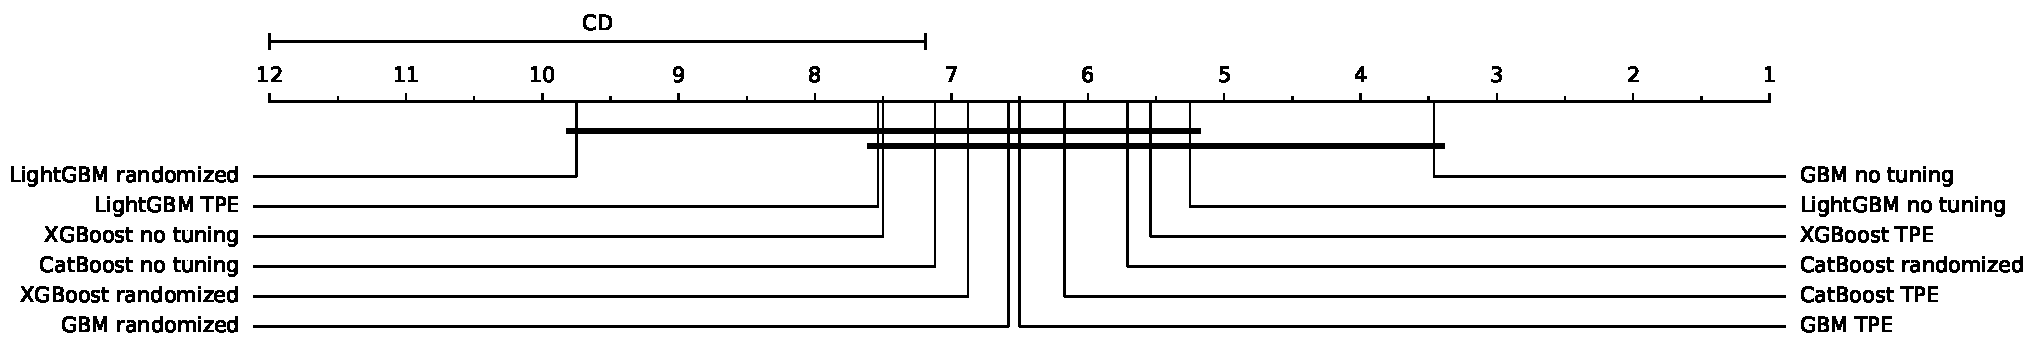
\includegraphics{main/plots/cd-cropped.pdf}}
	\caption{Critical difference plot of the accuracy ranks from Table~\ref{tab:all_tunings_rankings}}
	\label{fig:cd_plot}
\end{figure}

The visualization of ranks in Figure~\ref{fig:cd_plot} indicates that LightGBM tuned using randomized search and baseline GBM are models which performed much better and much worse than other variants, respectively. Only for these two aforementioned models the difference of their performance is statistically significant --- two bold horizontal lines connect models for which the aforementioned difference is insignificant. in Figure~\ref{fig:cd_plot} it can be observed that LightGBM TPE and baseline XGBoost are almost equally as good, a similar conclusions can be made for both tuned variants of GBM. Performance of XGBoost randomized is visibly worse compared to its baseline version --- the difference is even more significant in case of CatBoost and its tuned variants. Finally, enormous improvement of performance in case of LightGBM and GBM compared to their non-tuned versions can be observed.

\section{Choice of regularization hyperparametrization}\label{section:xgboost_regularization}
In GBM implementations, different hyperparameters which control regularization have been implemented. Proper regularization can greatly diminish the risk of overfitting, however, poor usage can lead to underfitting. Simultaneous usage of multiple regularization hyperparameters might not be optimal. Therefore, it is reasonable to check if it is necessary to use all of these hyperparameters at once.
XGBoost has been chosen to be used in the regularization analysis since it provides four hyperparameters related to regularization; the choice is the greatest among all four considered GBM implementations: GBM, XGBoost, LightGBM and CatBoost. In the analysis, three will be considered:
\begin{itemize}
\item $\alpha$, which is responsible for L1 regularization,
\item $\lambda$, which controls regularization in L2,
\item $\gamma$ or minimum loss reduction required to make a split.
\end{itemize}

Shrinkage $\nu$ also controls regularization, but it is an integral part of every possible gradient boosting implementation, thus it will not be considered.

In order to determine the proper choice of regularization hyperparametrization, a train test split have been performed on two datasets: \emph{prostate} and \emph{gina agnostic} --- they have been chosen because the high number of features suggests that some feature engineering will be needed in order for the model to perform optimally and not overfit. Both aforementioned datasets can be challenging to analyze without feature selection, because the number of features is high. Then, for different combinations of $\alpha$, $\lambda$ and $\gamma$, XGBoost has been fitted on the train set and then accuracy on the test set has been computed. Hyperparameters other than $\alpha$, $\lambda$ and $\gamma$ have been set to their respective default values. The results for the \emph{prostate} dataset have been presented in form of a heatmap in Figure~\ref{fig:regularization_prostate}.

\begin{figure}[H]
	\centering
		\scalebox{0.55}{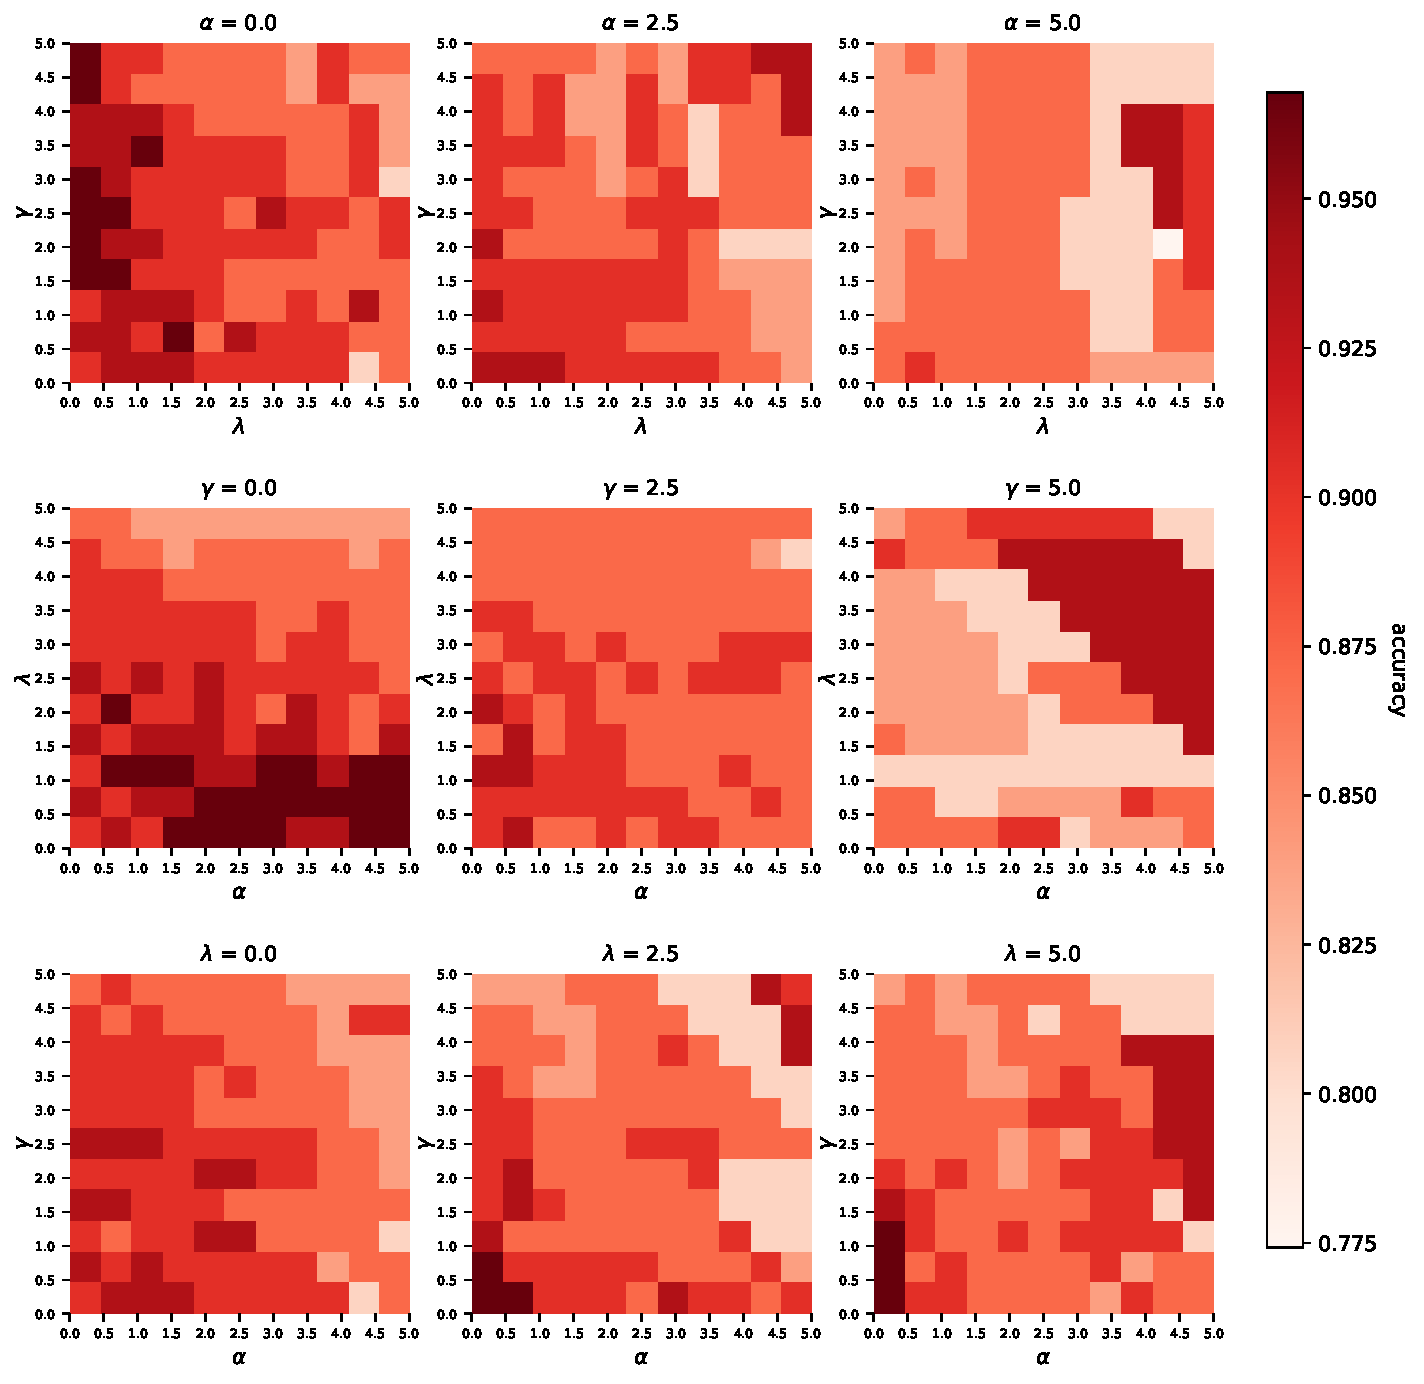
\includegraphics{main/plots/regularization_05_step_prostate.pdf}}
	\caption{XGBoost's accuracy on the test set --- \emph{prostate} dataset}
	\label{fig:regularization_prostate}
\end{figure}

Greater saturation of the color indicates higher accuracy on the test set. It can be observed that it is not necessary to set high values of $\alpha$, $\lambda$ and $\gamma$ simultaneously. High performance of the classifier can be obtained in the following ways:
\begin{itemize}
    \item by fixing low values of $\alpha$, $\lambda$ and changing the $\gamma$, e.g. $\alpha$ as well as $\lambda$ could be set to zero,
    \item by picking $\lambda$ from the interval $[0, 1]$, $\gamma=0$ and changing the value of $\alpha$,
    \item by fixing high $\lambda=5$ and picking low $\alpha$ and $\lambda$.
\end{itemize}

By taking high $\alpha$, $\lambda$ and $\gamma$ at the same time the performance of XGBoost can be degraded, each heatmap in the third column of the plot presented in Figure~\ref{fig:regularization_prostate} indicates that picking $\alpha=\lambda=\gamma=5$ is counterproductive. on the other hand, for $\gamma=5$ one could take $\alpha$ and $\lambda$ slightly lower than 5 and still get satisfying results. Similarly, high accuracy can be achieved by fixing $\alpha=5$ and taking higher values of $\lambda$ and $\gamma$.

In the case of the \emph{prostate} dataset, choosing only one hyperparameter among $\alpha$, $\lambda$ and $\gamma$ to have higher value might lead to a very decent generalization error. It is counter-intuitive, because the \emph{prostate} dataset has 6033 features, so it is reasonable to think that it would be difficult to achieve a good generalization error without choosing multiple regularization hyperparameters at once.

The aforementioned dataset's feature matrix is dense, thus the analysis has been repeated for a sparse one --- its results for the \emph{gina agnostic} dataset have been presented in Figure~\ref{fig:regularization_gina_agnostic}.

\begin{figure}[H]
	\centering
		\scalebox{0.55}{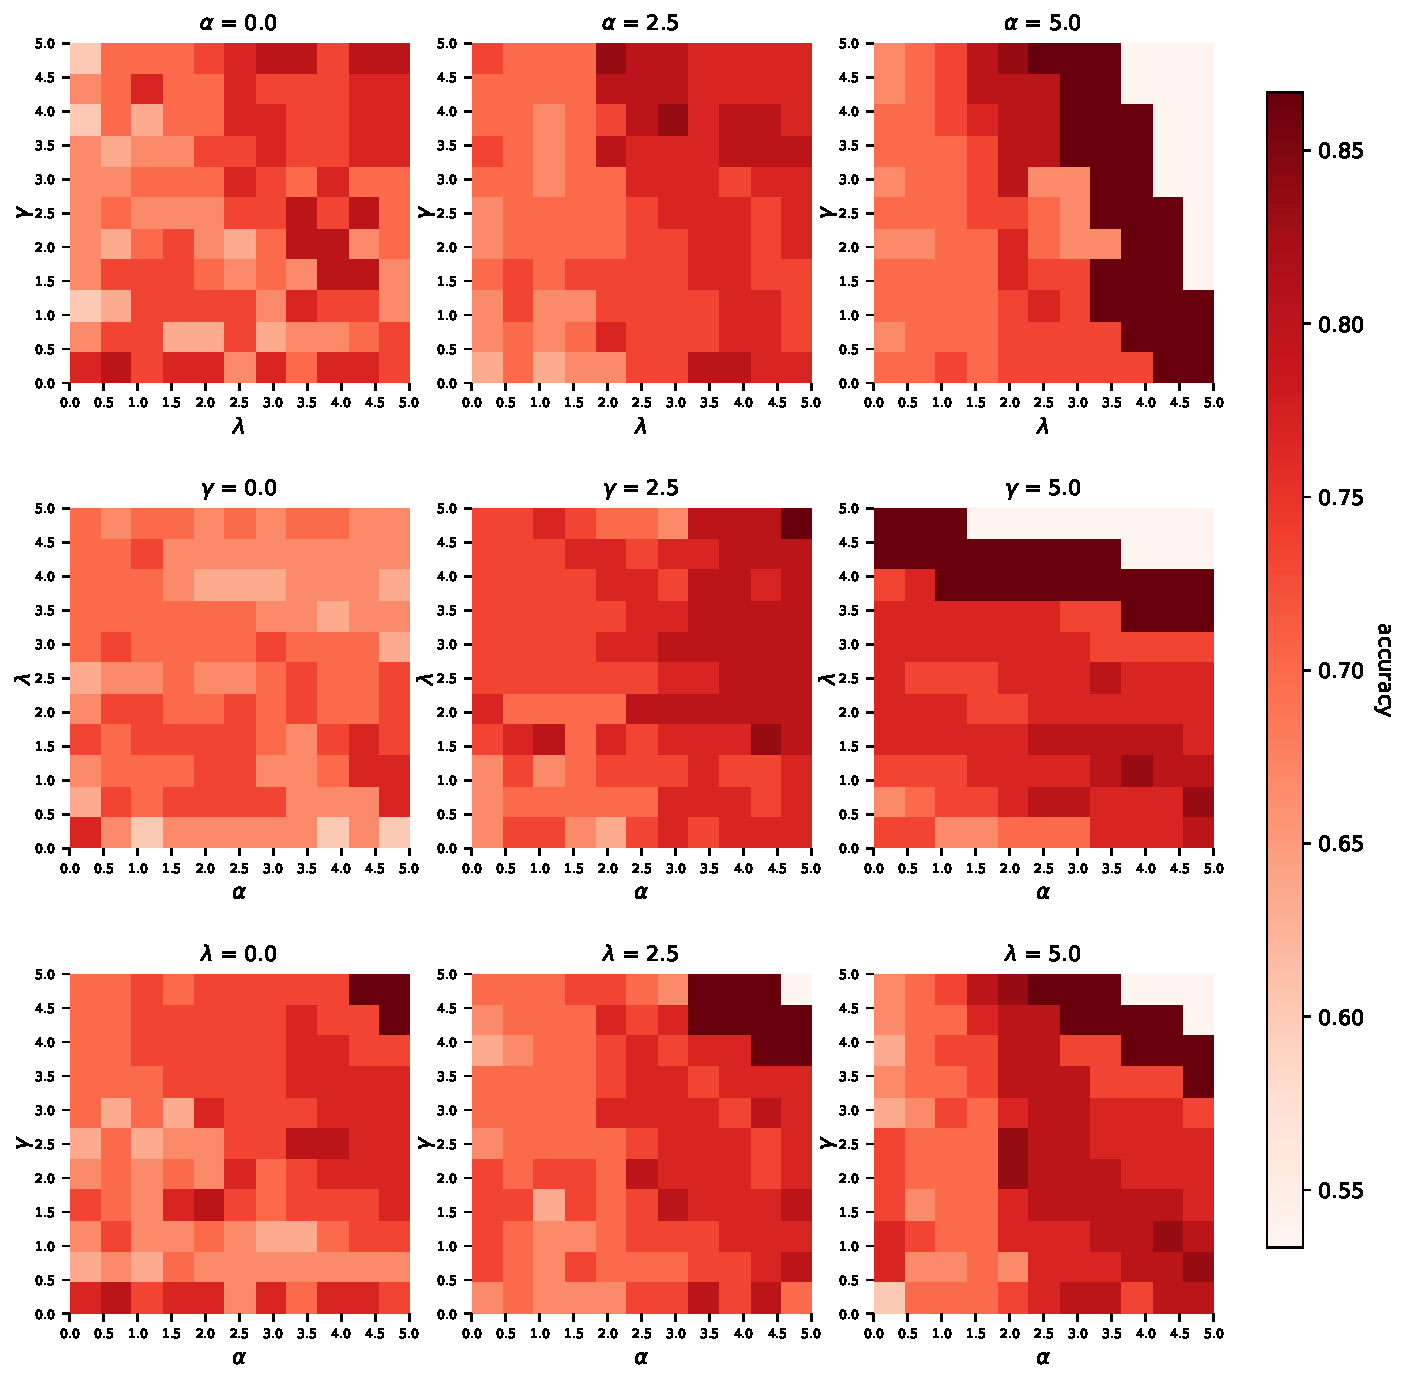
\includegraphics{main/plots/regularization_05_step_gina_agnostic.pdf}}
	\caption{XGBoost's accuracy on the test set --- \emph{gina agnostic} dataset}
	\label{fig:regularization_gina_agnostic}
\end{figure}

The results in case of a sparse dataset are quite different compared to those obtained in case of the \emph{prostate} dataset. For each heatmap, accuracy tend to increase when at least two regularization hyperparameters are also increasing, however, taking $\alpha=\lambda=\gamma=5$ will lead to a significant degradation in performance. Low regularization is not worth it, at least two hyperparameters among $\alpha$, $\lambda$ and $\gamma$ should be considered to obtain a satisfying generalization error.

In conclusion, regularization in GBM implementations can be tuned by adjusting the values of several hyperparameters. However, judging from the results presented in Figures~\ref{fig:regularization_prostate} and \ref{fig:regularization_gina_agnostic} regularization has to be considered on case-by-case basis. L1, L2 and $\gamma$ regularization may be more or less useful on different kinds of datasets. It is reasonable to perform hyperparameter tuning which will determine the optimal combination of regularization hyperparameters. When tuning is not computationally feasible, one should limit their choice to up to two aforementioned hyperparameters. However, since datasets exhibit different characteristics, the optimal choice of regularization hyperparameters should be researched separately in each use case.

\section{Impact of hyperparameter tuning on LightGBM}\label{section:lightgbm_tuning}
In Sections~\ref{section:baseline}, \ref{section_tpe} and \ref{section_rand} it has been proven that LightGBM which has been used using either Bayesian optimization with Tree Parzen Estimators or randomized search performs the best out of any tuned or not tuned GBM implementation. Therefore, it is reasonable to investigate in more detail the impact of different hyperparameters on LightGBM's performance.

The used parameter grid is similar to those displayed in the "LightGBM tuning" part of the Table~\ref{tab:init_tuning}. Hyperparameters which have been used in this experiment are:

\begin{itemize}
    \item number of leaves,
    \item learning rate,
    \item GOSS related hyperparameters: top rate and other rate,
    \item L1 and L2 regularization terms: $\alpha$ and $\lambda$.
\end{itemize}


The number of trees has been set to 150 and boosting type is GOSS. For each considered hyperparameter a list of ten values has been chosen and for each of those values the model's performance will be evaluated using 10-fold stratified cross-validation scheme. The purpose of the experiment is to check the sensitivity of LightGBM's performance when only a single value of a hyperparameter is modified.

In this experiment, all evaluations will be carried out on a simulated dataset\footnote{Documentation can be found here: \url{scikit-learn.org/stable/modules/generated/sklearn.datasets.make_classification.html}}. It is a dataset which enables to user to control the number of informative, redundant, repeated and noisy features as well as the "difficulty" of the classification task. It is an excellent benchmark dataset which can be used in evaluation of different Machine Learning models. The number of samples has been set to 10000, number of features to 20, \emph{class\_sep} which controls the separation between classes (complexity of classification task) has been set to 0.3. The labels are split into two classes with perfect balance. By using such aforementioned simulated dataset, one can directly control the number of discriminative features as well as avoid any peculiar data characteristics which occur in real data. The resulting boxplots for each model evaluation have been presented in Figure~\ref{fig:lightgbm_tuning}.

\begin{figure}[H]
	\centering
		\scalebox{0.6}{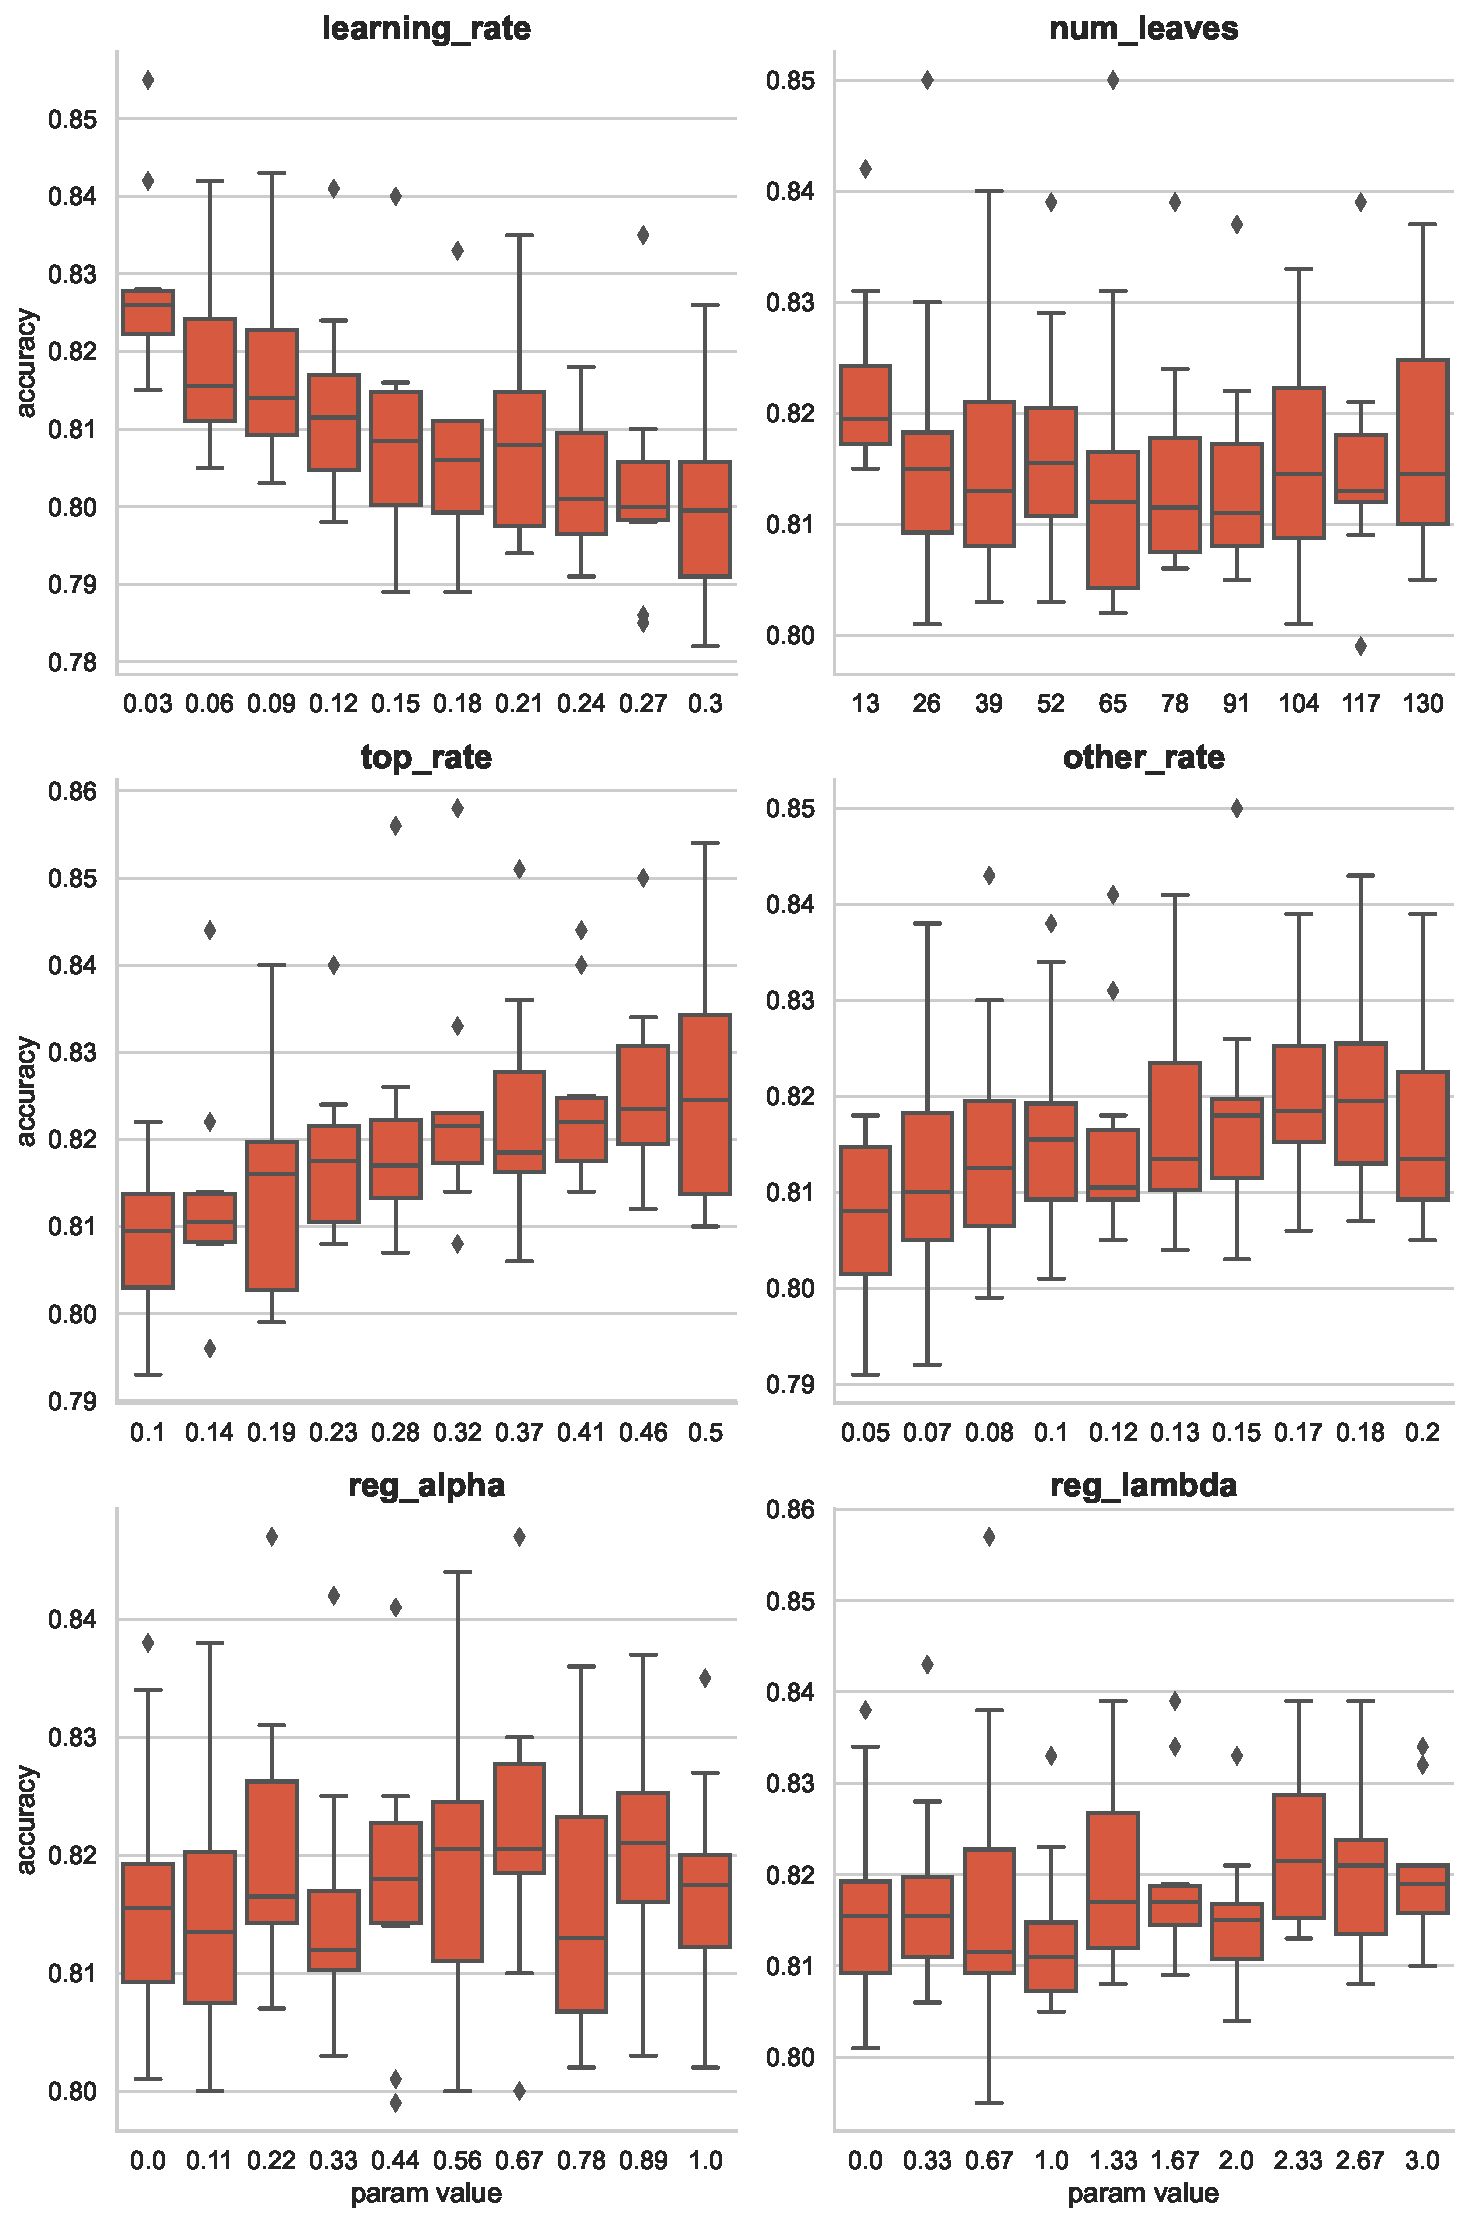
\includegraphics{main/plots/lightgbm_results_boxplots.pdf}}
	\caption{The impact of different hyperparameters on LightGBM's performance}
	\label{fig:lightgbm_tuning}
\end{figure}
\newpage
Generally, the change of the value of only one hyperparameter may lead to a significant change in model's accuracy. In case of the learning rate, the difference in performance when choosing either the lowest (0.03) or the highest (0.3) value can differ by almost 0.07 --- for the lowest learning rate, accuracy can be as high as 0.85. What is interesting is that the number of trees equal to 150 is not high, so it would be reasonable to think that a higher learning rate would perform better, but it is certainly not the case. The number of leaves also has a significant impact on model's performance. However, it can be observed that choosing less complex trees with only 65 or even 26 leaves would still yield satisfying (or even better) results. Most likely choosing the default value of 31 would also result in decent accuracy.

Accuracy seems to be an increasing function of GOSS hyperparameter \emph{top\_rate} (or retain ratio of large gradient data) --- choosing it as high as 0.5 will be the most beneficial. On the other hand, accuracy does not seem to be highly dependent on the value of \emph{other\_rate}. Moreover, regularization also has significant impact on the performance of the model. A proper choice of either $\alpha$ or $\lambda$ can lead to an increase of accuracy as high as 0.03. However, in case of $\alpha$ and $\lambda$ it would be difficult to choose values which are uniformly the best --- the case of each dataset is different.

Overall, it can be concluded that indeed LightGBM is quite sensitive to hyperparameter tuning. Choosing an appropiate value of only one hyperparameter may lead to a relatively significant increase in accuracy. Thus, it is not surprising that in the experiments which have been described in Sections~\ref{section:baseline}, \ref{section_tpe} and \ref{section_rand} tuned LightGBM was the best overall model among GBM, XGBoost, LightGBM and CatBoost. Great performance increase as well as computational efficiency and scalability of tuned LightGBM indicate that it has the best potential to be used in practical business use cases, which often demand very highly performing model and short computational time. In case of LightGBM, one could use a very big param grid or high number of iterations in Bayesian optimization or randomized search --- the time spent on tuning will not be that long, but it will be definitely worth it.

\section{Categorical encodings with CatBoost}\label{section:cat_comparison}
XGBoost, LightGBM and CatBoost are capable of categorical variables processing. However, in case of XGBoost, the aforementioned feature is experimental, so it cannot be relied on; according to the creatores of CatBoost \cite{catboost}, LightGBM's implementation of categorical encoding is not so effective. On the other hand, one CatBoost's main features is the ability to perform the encoding very well --- the importance of the categorical encoding has been emphasized greatly in the implementation paper \cite{catboost}.

In \cite{catboost} it has been mentioned that using the embedded encoding method alongside with the Ordered boosting type, one should avoid the prediction shift completely --- it that case, the random permutations of training examples $\sigma_{cat}$ used for encoding and for training $\sigma_{boost}$ will be the same: $\sigma_{cat} = \sigma_{boost}$. Thus, it is essential to determine if combining Ordered boosting with the embedded encoding algorithm in fact yields the best results. However, four different cases of the encoding will be considered:

\begin{itemize}
    \item Preprocessing of categorical variables using the CatBoost Encoder (not the CatBoost algorithm itself), which has been used in experiments in Sections~\ref{section:baseline}, \ref{section_tpe} and \ref{section_rand}; encoded features will be used with Ordered CatBoost.
    \item Embedded CatBoost encoding (using the \emph{cat\_features} argument) with Ordered boosting type.
    \item Embedded CatBoost encoding (using the \emph{cat\_features} argument) with Plain boosting.
    \item Preprocessing using standard One-Hot-Encoding (OHE) with Ordered boosting type.
\end{itemize}

Two benchmark datasets which contain categorical features only have been used: \emph{mushrooms} and \emph{amazon} --- they have been described in Table~\ref{tab:datasets}. Model evaluation has been performed by 10-fold stratified cross-validation scheme; the metrics of choice were accuracy, AUC and negative log loss (originally, log loss should be as low as possible, but to retain the convention that higher metric value implies greater performance, the values of log loss have been multiplied by $-1$). The distributions of the metrics values across both aforementioned datasets have been presented in Figure~\ref{fig:catboost_categorical_results}.

\begin{figure}[H]
	\centering
		\scalebox{0.47}{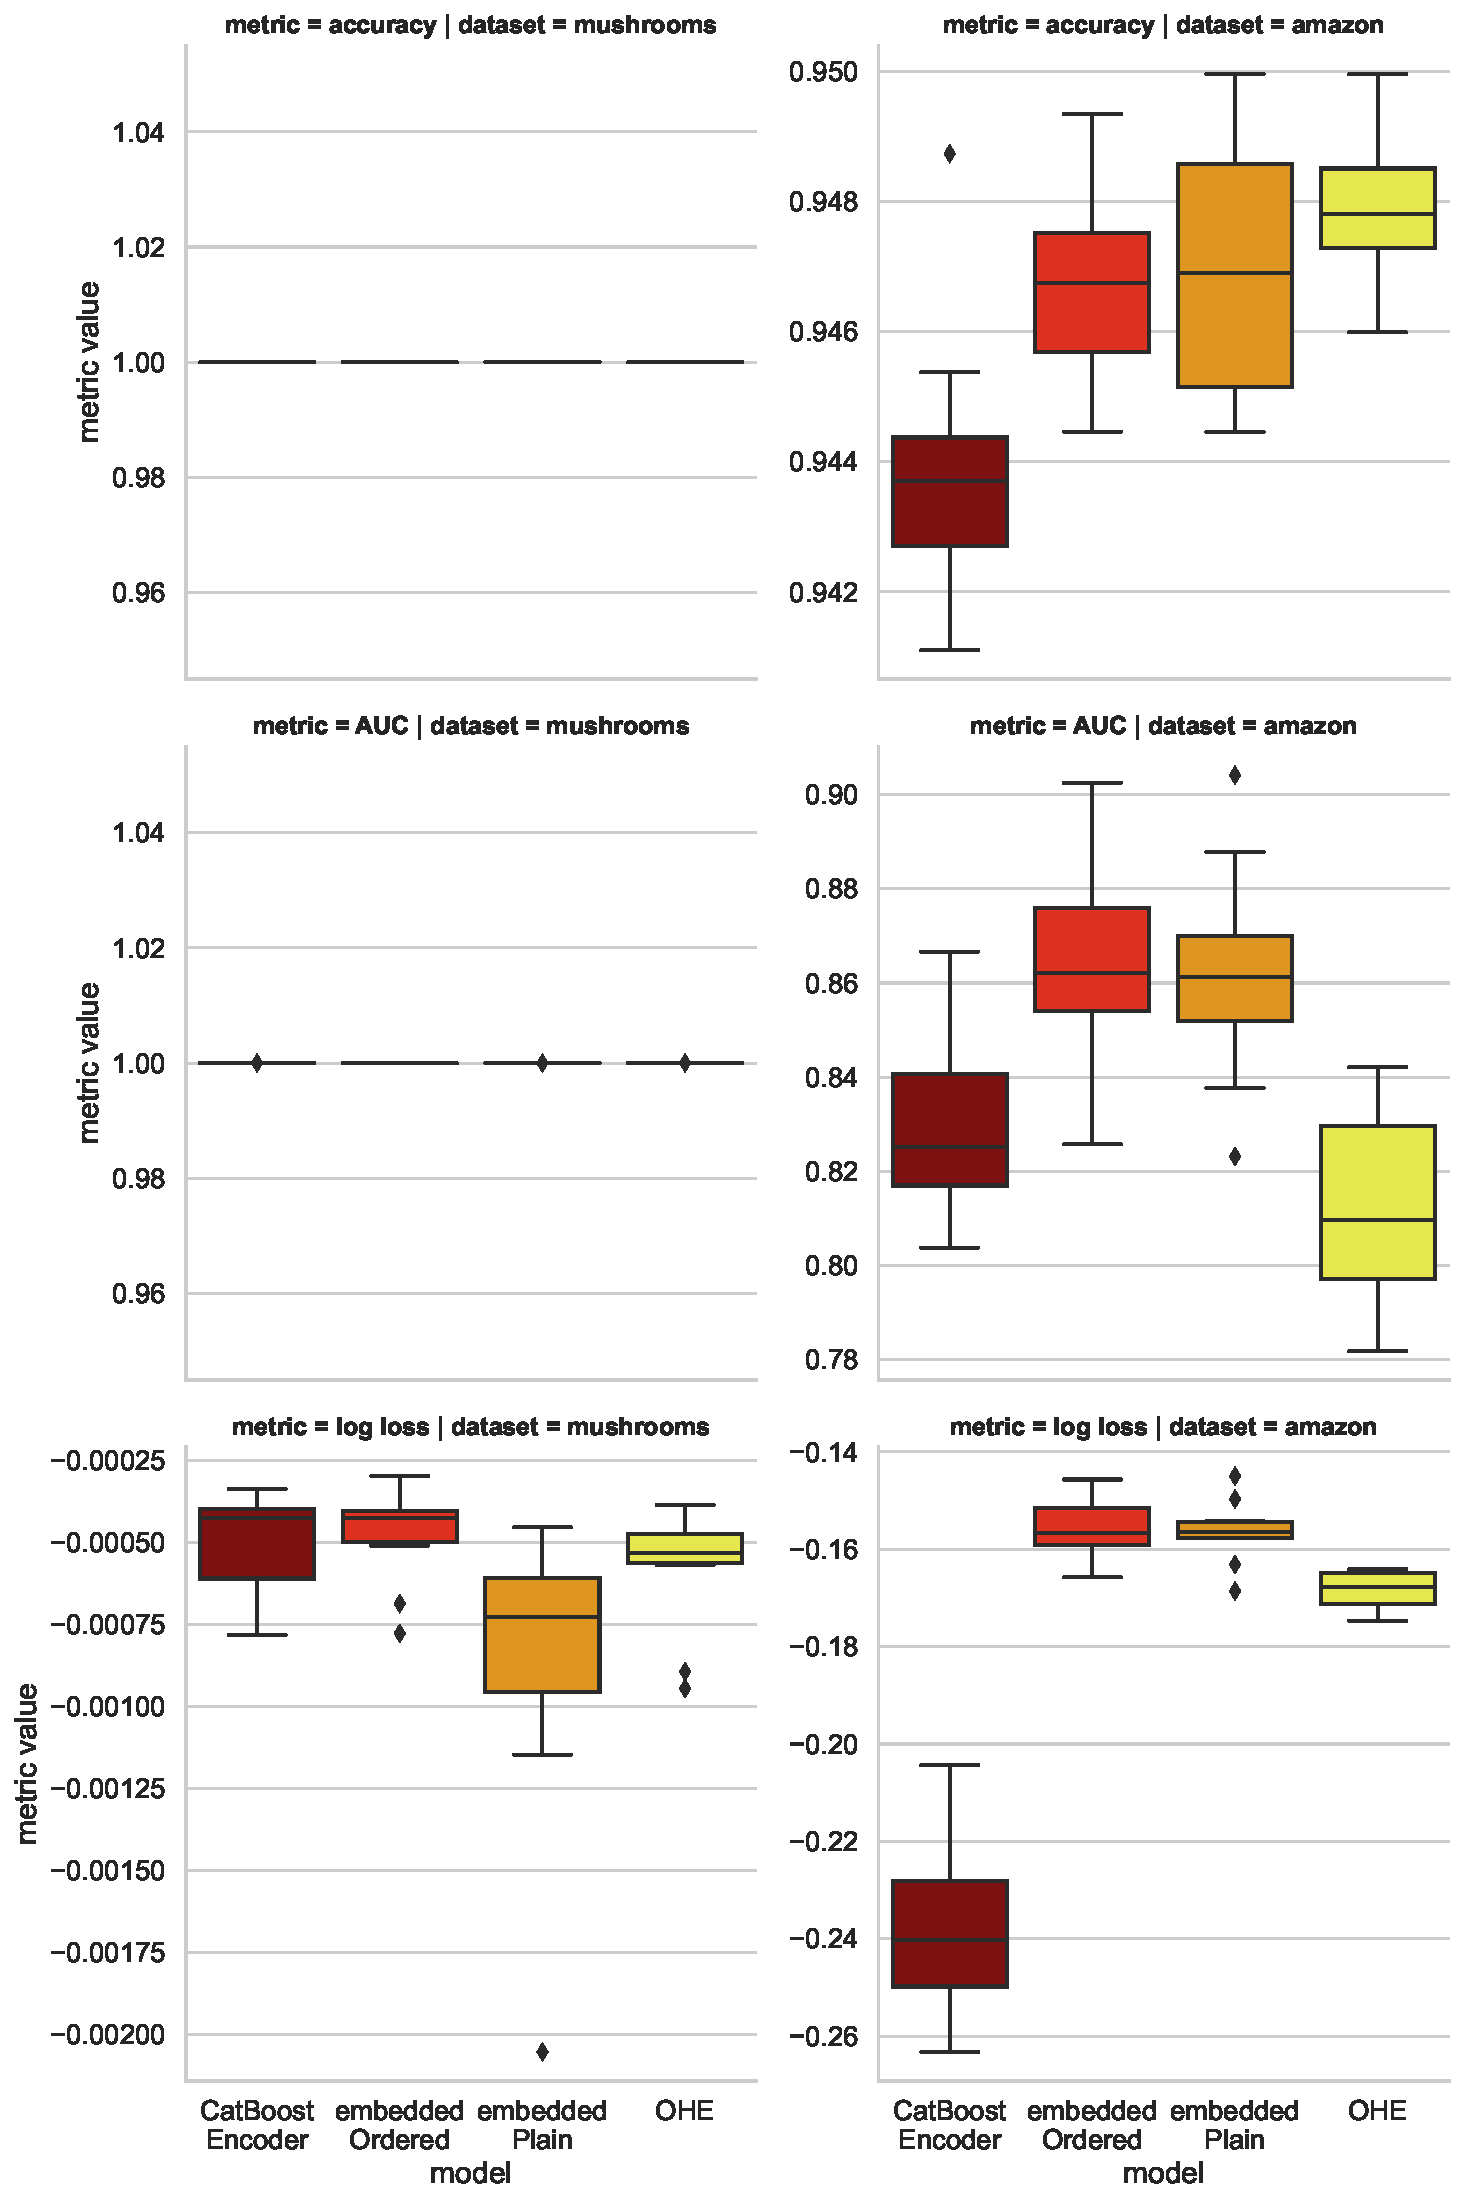
\includegraphics{main/plots/catboost_results_all_metrics.pdf}}
	\caption{Accuracy, AUC and negative log loss distributions across \emph{mushrooms} and \emph{amazon} datasets}
	\label{fig:catboost_categorical_results}
\end{figure}

In case of the \emph{mushrooms} dataset, the performance of all methods of encoding is almost equal. A difference can be only observed in the case of log loss metric --- embedded encoding with Ordered CatBoost seems to yield the lowest values of the log loss (or the highest values of the negative log loss). The situation is different on the \emph{amazon} dataset --- in terms of accuracy, Ordered CatBoost with features encoded using One-Hot-Encoding seems to perform the best. The embedded encoding algorithm used with Plain CatBoost is also a decent option, but it is less stable than OHE. Ordered CatBoost with equal random permutations $\sigma_{cat} = \sigma_{boost}$ seems to be worse than both Plain embedded CatBoost and OHE which is quite surprising. Preemptive preprocessing of data using CatBoost Encoder is most likely the worst option; overall, in terms of accuracy, all encoding methods performed very similarly. Similarly to the \emph{mushrooms} dataset, embedded encoding with Ordered CatBoost also performs the best in terms of log loss metric -- this result coincides with these obtained by authors of CatBoost in \cite{catboost}, where it has been shown that taking equal categorical and training permutations $\sigma_{cat} = \sigma_{boost}$ leads to a minor decrease of log loss value.

Embedded Ordered CatBoost yields the best performance in terms of AUC score, while One-Hot-Encoding paired with Ordered CatBoost is the worst. AUC between all four types of encoding seems to differ a lot, there is a significant upgrade in performance when using Ordered CatBoost with equal random permutations $\sigma_{cat} = \sigma_{boost}$. The runtimes of all encoding methods have been presented in Figure~\ref{fig:catboost_categorical_runtimes}.

\begin{figure}[H]
	\centering
		\scalebox{0.5}{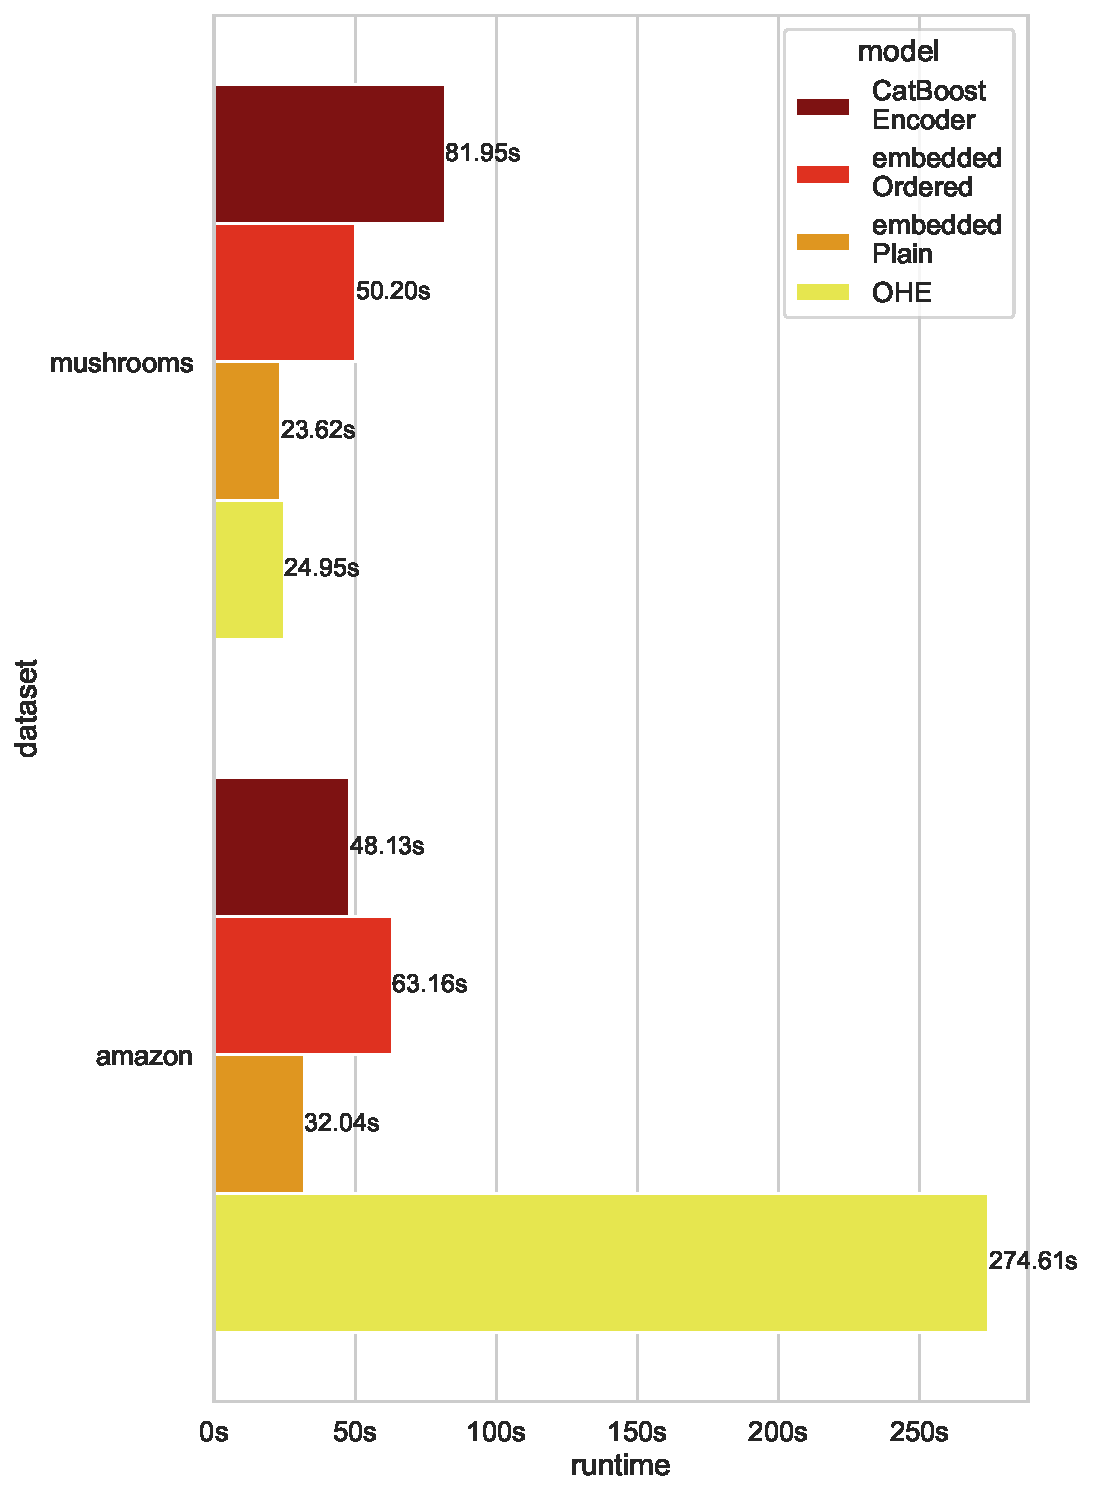
\includegraphics{main/plots/catboost_runtimes.pdf}}
	\caption{Runtimes across \emph{mushrooms} and \emph{amazon} datasets}
	\label{fig:catboost_categorical_runtimes}
\end{figure}

As it was expected, CatBoost with OHE takes a long time to run --- the \emph{amazon} dataset originally has only 9 features, but after performing OHE, the number increases to 15626. Thankfully, the features are sparse, thus CatBoost's runtime is not that long. The runtimes in the case of \emph{mushrooms} dataset are much more even. In case of both datasets, it is advised to use the embedded categorical encoding methods, either with Ordered (if the time permits) or Plain boosting type. CatBoost's implementation of categorical encoding works well, it is fast and very easy to use.

CatBoost is the preferred GBM implementation to use with categorical datasets, however, the CatBoost Encoder, which preemptively processes the variables without using CatBoost itself is also a viable option.

\chapter{Conclusions and final remarks}\label{chapter:conclusions}
In this chapter, the results of the comparative analysis which have been presented in Chapter~\ref{chapter:results} will be compared to those described in the literature regarding four GBM implementations: GBM~\cite{friedman_gbm}, XGBoost~\cite{xgboost}, LightGBM~\cite{lightgbm} and CatBoost~\cite{catboost}. Additionally, recommendations regarding choosing the most appropriate GBM algorithm will be given as well as final remarks regarding this study will be highlighted.

\section{Discussion of results and conclusions}
Overall, the results obtained from comparative experiments presented in Sections~\ref{section:baseline}, \ref{section_tpe} and \ref{section_rand} tend to differ from those described in \cite{comparative_analysis}, \cite{competitive_analysis} and \cite{comparison_of}.

In this work, we have concluded that LightGBM tuned using either Bayesian optimization or randomized search was the best GBM algorithm in terms of an average rank across twelve datasets. Due to excellent performance, very low fitting time and the number of useful hyperparameters tuned LightGBM has the biggest potential if used mindfully. On the other hand, authors of \cite{comparative_analysis} have stated that CatBoost tuned using grid search procedure was the best model in terms of accuracy --- however, its rank was statistically insignificant compared to other models (in our study, only the difference of performance of tuned LightGBM and baseline gradient boosting was confirmed to be statistically significant). Also, in \cite{comparative_analysis} it has been stated that the performance of tuned and baseline variants of CatBoost was very similar --- on the other hand, in this work we have proven that performing hyperparameter search with CatBoost is counterproductive; its baseline variant has proven to perform much better in terms of accuracy, F1 score and AUC. In \cite{comparative_analysis} authors have mentioned that CatBoost need not to be tuned to achieve competitive performance which coincides with the results obtained in this work.

Both in \cite{comparative_analysis} and in our analysis baseline LightGBM is one of the worst GBM variants in terms of performance. However, we have proven that baseline XGBoost is one of the best algorithms in terms of average ranks in case of F1 score and AUC (rank 3 and 4, respectively) --- in \cite{comparative_analysis} the authors have shown that baseline XGBoost performs poorly, which is surprising. Interestingly, tuned GBM turned out to be the best performing algorithm alongside tuned CatBoost and XGBoost, while in our study it has been ranked sixth or seventh out of twelve algorithms in terms of average rank. Additionally, GBM in this work was clearly the worst performing GBM implementation, but in \cite{comparative_analysis} it outperformed baseline variants of XGBoost and LightGBM. The differences between the results obtained in our comparative analysis and in \cite{comparative_analysis} could be caused by several different aspects of designed evaluation procedures. Firstly, in \cite{comparative_analysis} a train-test split approach has been employed with 10-fold cross-validation scheme used for grid search based hyperparameters tuning. Secondly, even though the number of used datasets was larger (28 compared to 12 analyzed in this work) the data diversity was not as significant, especially in terms of the number of features (authors of \cite{comparative_analysis} did not include highly dimensional datasets, such as those where the number of features was much higher than the number of samples).

In \cite{competitive_analysis} CatBoost was deemed as the best accurate implementation compared to XGBoost, LightGBM and SnapBoost and it has been stated that it performed the best in case of the categorical dataset --- in our study, that was not the case for both \emph{amazon} and \emph{mushrooms} datasets. Additionally, in \cite{competitive_analysis} XGBoost, LightGBM and CatBoost all greatly benefited from hyperparameter tuning while it was not confirmed in our analysis --- even though in both cases Bayesian optimization was used, different search spaces have been provided; additionally, authors of \cite{competitive_analysis} have utilized the train-test split instead of the double cross-validation procedure proposed in this work.

On the other hand, some some of our findings coincide with those presented in \cite{comparison_of}. In \cite{comparison_of} it has been concluded that among tuned variants of XGBoost, LightGBM and CatBoost LightGBM performed the best both in terms of accuracy and runtime. Additionally, in \cite{comparison_of} CatBoost was the algorithm which benefited the most from hyperparamerer tuning --- overall, it was never the case that a baseline variant of XGBoost, LightGBM or CatBoost was better than their tuned counterparts; the tuning always increased the accuracy of the models.
In terms of model fitting time, the results presented in the literature: \cite{comparative_analysis}, \cite{competitive_analysis}, \cite{comparison_of} as well as \cite{lightgbm} tend to coincide with our conclusions --- LightGBM is always the fastest algorithm, no matter if the GOSS sampling is used or not. Additionally, in this work we have shown that the runtime of CatBoost (both Plain and Ordered variants) is heavily dependent on the dimensionality of the data, but not on the number of features. CatBoost's runtime is quite low for datasets with moderate number of features and very high in case of highly dimensional data --- such conclusion is not consistent with the literature, where the overall consensus is that CatBoost, especially its Ordered variant is the slowest (although most of the datasets which have been considered in the literature have low to moderate number of features).

Moreover, in our study we have shown that XGBoost (with the exact greedy splitting algorithm) tends to perform inconsistently in terms of runtime across different datasets. However, it was sometimes faster than both CatBoost and GBM. The results presented in the literature are not conclusive, because sometimes, the histogram version of XGBoost has been used \cite{lightgbm}, \cite{comparison_of} --- then, the runtime of the algorithm is more comparable, even to the average runtime of LightGBM. Thus, since XGBoost offers many options regarding the splitting algorithm (i.e. exact, approximate and histogram), in practice it is reasonable to verify the performance of all three aforementioned variants.

The ease of use is also a relevant consideration when using GBM~\cite{friedman_gbm}, XGBoost~\cite{xgboost}, LightGBM~\cite{lightgbm} and CatBoost~\cite{catboost}. It was only mentioned in \cite{comparison_of}, however, in this work we came up with our own conclusions. Overall, the simplest algorithm to use is the basic GBM --- it has the least number of available hyperparameters and in the context of programming effort, its implementation is available in the scikit-learn library \cite{sklearn}, so no external packages need to be installed. However, in applications it is essential to maintain a decent level of model's performance (since we have proven that GBM is not as effective as XGBoost, LightGBM or CatBoost), so an algorithm which is easy to use should also be effective. We have shown that baseline variants of XGBoost and CatBoost perform very well --- they work great "out of the box", and this makes them the easiest algorithms to use. LightGBM needs to be tuned in order to achieve high performance, thus it should not be deemed as easy to use.

In terms of the number of available hyperparameters, LightGBM offers the biggest variety. There are a lot of hyperparameters available both in XGBoost and LightGBM, but the number of possible configurations in XGBoost is not as high as in the case of LightGBM. CatBoost offers the least number of available hyperparameters, but they are often unique and cannot be found in any other GBM implementation. However, CatBoost offers the least amount of information available in the documentation; on the other hand, XGBoost and LightGBM offer much more exhaustive descriptions of hyperparameters. Thus, when considering hyperparameter tuning, we have concluded that XGBoost would be the easiest to use; the second easiest GBM implementation would be LightGBM. We advise that LightGBM should be used by experienced researchers who know the ins and outs of gradient boosting algorithms and the specifics of LightGBM. However, none of GBM, XGBoost or LightGBM offer robust support of categorical and text variables --- in this context, CatBoost is the clear winner; the user only has to specify which columns contain categorical or text variables.

The recommendations regarding the choice of the optimal GBM implementation depends on many factors --- a summary diagram has been presented in Figure~\ref{fig:recommendations}. To summarize, XGBoost and CatBoost are the best algorithms when baseline variants are considered and all models: GBM, XGBoost, LightGBM and CatBoost can be said to perform well in the case when hyperparameter tuning is performed. LightGBM was the only model with inconsistent performance (i.e. the spread or standard deviations of the evaluation metrics were high), while GBM and LightGBM were very consistent in terms of runtime across different datasets (to recall, the runtime of XGBoost and CatBoost was highly sensitive to the number of features).

In terms of scalability, due to the incorporation of L1 and L2 regularization XGBoost and LightGBM should be the primary choices when considering datasets with high number of features. GBM does not scale well with the number of samples (since it hardly implements any mechanisms which may reduce the runtime) --- XGBoost, LightGBM and CatBoost seem to process large number of samples quite well. Also, sparsity-aware splitting algorithms implemented in XGBoost and LightGBM help to significantly decrease the training time in case of sparse datasets, thus we suggest using them instead of GBM or CatBoost, (GBM and CatBoost never addressed the aspect of data sparsity).  When the number of samples is very large, then LightGBM or histogram variant of XGBoost should be used. Moreover, XGBoost and LightGBM offer the widest range of available hyperparameters and most of them are very well documented. The implementation of GBM available in scikit-learn \cite{sklearn} also has excellent documentation; additionally, since GBM \cite{friedman_gbm} was the original gradient boosting algorithm, it should be the most recognizable among researchers. For users who are not as knowledgeable about gradient boosting algorithms, XGBoost and CatBoost will be the best choice due to their excellent "out of the box" performance.

In Section~\ref{section:xgboost_regularization} we have concluded that it might not be optimal to consider multiple regularization hyperparameters at once in the case of XGBoost. It is not worth to use $\alpha$, $\lambda$ and $\gamma$ simultaneously. On the other hand, the usage of aforementioned hyperparameters is highly specific to the considered dataset, no matter which GBM implementation we will choose. We recommend a careful approach, since improper regularization can lead to either under- or overfitting. Additionally, one should consider the interactions between hyperparameters; for example, in case of XGBoost the deeper the trees are, the more aggressive $\gamma$-pruning should be used and thus higher $\gamma$ should be chosen.

In Section~\ref{section:lightgbm_tuning} we have analyzed the impact of hyperparameter tuning on LightGBM. Using simulated data we have shown that a change of only one hyperparameter's value can lead to an increase in performance in terms of accuracy by a few percentage points. We have concluded that LightGBM is quite sensitive to tuning, thus it is worth it to perform hyperparameter search. It is also crucial to mindfully choose the values for \emph{top\_rate} and \emph{other\_rate} hyperparameters used when GOSS sampling is used --- we have shown that generally, model's performance slightly increases when their values are higher (it coincides with the literature --- in \cite{comparative_analysis} a similar conclusion was made). However, the user should be familiar with the implementation of LightGBM \cite{lightgbm} and the GOSS algorithm, because by default it is disabled in the implementation.

Finally, in Section~\ref{section:cat_comparison} we have compared different methods of categorical variable encoding. We considered two categorical datasets and in their case we have shown that in terms of log loss metric, it is absolutely recommended to use Ordered CatBoost with its embedded Ordered TS categorical encoding algorithm --- this results is inline with the recommendations given by the authors of CatBoost \cite{catboost}. Additionally, we have shown that using One-Hot Encoding is counterproductive --- in case of datasets with variables with high cardinality, the number of features to consider in each split greatly increases, thus the computational demands become much higher.

\begin{sidewaysfigure}
	\centering
		\scalebox{0.72}{\includegraphics{main/plots/recommendations.pdf}}
	\caption{The choice of optimal GBM implementation in different scenarios. Drawn using \emph{draw.io}}
	\label{fig:recommendations}
\end{sidewaysfigure}

\newpage
\section{Final remarks}
In this work, we have managed to successfully perform a comparative analysis of four gradient boosting algorithms: GBM~\cite{friedman_gbm}, XGBoost~\cite{xgboost}, LightGBM~\cite{lightgbm} and CatBoost~\cite{catboost}. Firstly, we have carefully reviewed and analyzed the results regarding the performance of aforementioned GBM implementations which have been recently presented in the literature. Then, we have laid solid theoretical foundations for classification and each considered gradient boosting implementation. Finally, we have carried out an comprehensive comparative analysis of GBM, XGBoost, LightGBM and CatBoost as well as we have analyzed the selected advanced aspects of XGBoost, LightGBM and CatBoost. We have shown that all considered variants of gradient boosting perform exceptionally well, both in terms of evaluation metrics, such as accuracy, F1 score or AUC score and runtime. However, in most of the cases some GBM implementations might be a better choice than other. Although some general recommendations regarding choosing the best gradient boosting algorithm can be given, each use case is highly individual. Thus, it is essential to consider models which suit peculiar data characteristic --- specific recommendations have been given in this work. Still, the choice of an optimal GBM implementation remains an open problem; in applications, an experienced researcher will be able to determine the right choice and use gradient boosting algorithms to its full potential.

\newpage
\nocite{*}
\bibliografia{bibliografia}

\begin{appendices}\label{appendix}
\chapter*{Appendix}
The version of \emph{Python} used in the experiments is 3.9.6.
Packages containing gradient boosting implementations, Bayesian optimization framework and categorical variables encoding algorithm are the following:

\begin{itemize}
\item scikit-learn==1.0.2
\item xgboost==1.5.2
\item lightgbm==3.3.2
\item catboost==1.0.4
\item tune-sklearn==0.4.1
\item ray[tune]==1.10.0
\item hyperopt==0.2.7
\item category\_encoders==2.4.1
\end{itemize}

Full repository containing all programs, plots, results and other files can be found at \url{github.com/243046/boost}. Two notebooks as well as one module are the most important:
\begin{itemize}
\item colab/colab\_experiments\_TPE.ipynb
\item colab/colab\_experiments\_randomized.ipynb
\item models/classifiers.py
\end{itemize}
\end{appendices}



\end{document} 